% This is the main file for the template for doctoral thesis at
% University of Zagreb, Faculty of Electrical Engineering and Computing
% in Zagreb, Croatia.
% Initial version was created in April 2013, last update was in July 2014.

% Author: Jelena Bozek, jelena.bozek@fer.hr
% Contributor: Vedran Miletic, vmiletic@inf.uniri.hr


%%%%%%%%%%%%%%%%%%%%%%%%% POSTAVKE / SETTINGS %%%%%%%%%%%%%%%%%%%%%%%%%%%%%
\documentclass[12pt,oneside, a4paper]{book}
\usepackage{etex}
%\usepackage{xcolor}
\usepackage[pdftex]{graphicx}
\usepackage{rotating}
\usepackage{epsfig}
\usepackage{epstopdf}
\usepackage[table]{xcolor}% http://ctan.org/pkg/xcolor
\usepackage{tikz}
\usetikzlibrary{positioning}
\usetikzlibrary{calc}
\usetikzlibrary{shapes.geometric, arrows, arrows.meta}
\usetikzlibrary{shadows,trees, mindmap}
\usetikzlibrary{matrix}
\usetikzlibrary{fit}
% required for printing index
% use \index{name} in text
%\usepackage{makeidx}
%\makeindex
% required for printing nomenclature
% use \nomenclature{symbol}{description} in text
%\usepackage{nomencl}
%\makenomenclature
%\renewcommand{\nomname}{Popis oznaka}

\usepackage[T1]{fontenc}
\usepackage[utf8]{inputenc}
\usepackage{cmap}
\usepackage[english]{babel}
\usepackage{ae}
\usepackage[unicode, hidelinks]{hyperref}
\usepackage{mathptmx}
\usepackage{amscd}
\usepackage{amssymb}
\usepackage{amsmath}
\usepackage{bm}
\usepackage{algpseudocode}
\usepackage{algorithm}
\renewcommand{\thealgorithm}{\arabic{chapter}.\arabic{algorithm}} 
\usepackage{bookmark}
% for making examples of comments
\usepackage{comment}

\usepackage{color,soul}
\definecolor{light-gray}{gray}{0.95} 
\DeclareRobustCommand{\hlcyan}[1]{{\sethlcolor{cyan}\hl{#1}}}
\DeclareRobustCommand{\hlgreen}[1]{{\sethlcolor{green}\hl{#1}}}

\newtheorem{mydef}{Example}[section]
\usepackage{amsfonts}
\usepackage{booktabs}

\usepackage[inline]{enumitem}

\setlist[description]{leftmargin=3cm,labelindent=\parindent}
\makeatletter
\def\namedlabel#1#2{\begingroup
    #2%
    \def\@currentlabel{#2}%
    \phantomsection\label{#1}\endgroup
}

% editing a cell 
% https://tex.stackexchange.com/questions/2441/how-to-add-a-forced-line-break-inside-a-table-cell/19678
\usepackage{makecell}
\renewcommand\theadalign{bc}
\usepackage{xspace}

\DeclareMathOperator*{\argmax}{arg\,max}
\DeclareMathOperator*{\argmin}{arg\,min}


\newcommand{\ComArg}{\mbox{\textsc{ComArg}}\xspace}

\colorlet{orangegreen}{green!10!orange!90!}
\definecolor{darkgreen}{rgb}{0, 0.5, 0} 

% for tables in clustering section
\newcommand{\str}[1]{{\scriptsize\emph{#1}}}

% pro and con colors
\newcommand{\pro}[1]{\textcolor{darkgreen}{#1}}
\newcommand{\con}[1]{\textcolor{red}{#1}}

\newcommand{\todo}[1]{\textcolor{red}{TODO: #1}}

\usepackage[left=2.5cm,right=2.5cm,top=2.5cm,bottom=2.5cm]{geometry}
\usepackage{setspace} 
\linespread{1.3}
\usepackage{fancyhdr} % setting up header and position of page numbers
\pagestyle{fancyplain}
\fancyhf{}
\lhead{\nouppercase{\fancyplain{}{\leftmark}}}
\renewcommand{\chaptermark}[1]{\markboth{#1}{}}
\rfoot{\thepage}

\usepackage{minted}
\usepackage{listings}
\usepackage{hhline}
%\usepackage{enumerate}
\usepackage{delarray}
\usepackage{array}  % package for some table properties
\usepackage{tabularx} % package that allows dynamical changing table cell width
\usepackage{multirow}  % package that enables multiple rows in a table
\usepackage[bf, font=small]{caption}
\usepackage[labelfont=small, font=small]{subcaption}
\usepackage{wasysym}
\usepackage{subeqnarray}
\usepackage{aeguill}
\usepackage{pdflscape} % setting page into landscape view
\setlist{nolistsep}   % setting for itemize lists

\usepackage[toc,page]{appendix}

%\renewcommand{\thefootnote}{\fnsymbol{footnote}}  % to get unnumbered footnotes
\renewcommand{\arraystretch}{1.5} % stretching row height

% roman numbers
\newcommand*{\rom}[1]{\expandafter\@slowromancap\romannumeral #1@}

\newcounter{rowcntr}[table]
\renewcommand{\therowcntr}{\thetable.\arabic{rowcntr}}

% A new columntype to apply automatic stepping
\newcolumntype{N}{>{\refstepcounter{rowcntr}\therowcntr}c}

% Reset the rowcntr counter at each new tabular
\AtBeginEnvironment{tabular}{\setcounter{rowcntr}{0}}

% use with numbered citations
%\usepackage[square, numbers, comma, sort]{natbib} 
\usepackage[round, comma, sort]{natbib} 
%\usepackage{natbib} 
% change the name of Bibliography heading into "Literatura"
% \addto\captionscroatian{%
%   \renewcommand{\bibname}{Bibliography}
% }

% Adding a dot after chapter number in TOC 
\let\savenumberline\numberline
\def\numberline#1{\savenumberline{#1.}}

% Adding dots after chapter titles to page number in TOC
\makeatletter
\renewcommand*\l@chapter[2]{%
  \ifnum \c@tocdepth >\m@ne
  \addpenalty{-\@highpenalty}%
  \vskip 1.0em \@plus\p@
  \setlength\@tempdima{1.5em}%
  \begingroup
  \parindent \z@ \rightskip \@pnumwidth
  \parfillskip -\@pnumwidth
  \leavevmode \bfseries
  \advance\leftskip\@tempdima
  \hskip -\leftskip
  #1\nobreak\normalfont\leaders\hbox{$\m@th
    \mkern \@dotsep mu\hbox{.}\mkern \@dotsep
    mu$}\hfill\nobreak\hb@xt@\@pnumwidth{\hss #2}\par
  \penalty\@highpenalty
  \endgroup
  \fi}
\makeatother

% adjust the line spacing in a matrix
\makeatletter
\renewcommand*\env@matrix[1][\arraystretch]{%
  \edef\arraystretch{#1}%
  \hskip -\arraycolsep
  \let\@ifnextchar\new@ifnextchar
  \array{*\c@MaxMatrixCols c}}
\makeatother

% remove footer (page number) from TOC, list of figures and list of tables
\AtBeginDocument{\addtocontents{toc}{\protect\thispagestyle{empty}}}
\AtBeginDocument{\addtocontents{lof}{\protect\thispagestyle{empty}}}
\AtBeginDocument{\addtocontents{lot}{\protect\thispagestyle{empty}}}

% enumerated description: 
% https://tex.stackexchange.com/questions/30029/enumerated-description-list
\newcounter{descriptcount}
\newlist{enumdescript}{description}{2}
\setlist[enumdescript,1]{%
  before={\setcounter{descriptcount}{0}%
	  \renewcommand*\thedescriptcount{(\arabic{descriptcount})}}
  ,font=\bfseries\stepcounter{descriptcount}\thedescriptcount~
}
% \setlist[enumdescript,2]{%
%   before={\setcounter{descriptcount}{0}%
%           \renewcommand*\thedescriptcount{\roman{descriptcount}}}
%   ,font=\bfseries\stepcounter{descriptcount}\thedescriptcount~
% }

% references in words, chapter one opposed to chapter 1
\usepackage{fmtcount,refcount}

\begin{document}

%%%%%%%%%%%%%%%%%%%%%%%%%%%%%%%%%%%%%%%%%%%%%%%%%%%%%%%%%%%%%%%%%%%%%%%%%%%
% titlepage
%%%%%%%%%%%%%%%%%%%%%%%%%%%%%%%%%%%%%%%%%%%%%%%%%%%%%%%%%%%%%%%%%%%%%%%%%%%
\frontmatter

%%%%%%%%%%%%%%%%%%%% NASLOVNICA / FRONT COVER PAGE %%%%%%%%%%%%%%%%%%%%%%%%
\begin{titlepage}
  \fontsize{16pt}{20pt}\selectfont
  \fontfamily{phv}\fontseries{mc}\selectfont
  \newgeometry{left=3cm,right=3cm,top=3cm,bottom=2.5cm}
  \setlength{\intextsep}{0pt plus 0pt minus 0pt}

  \begin{center}
    \begin{figure}[ht!]
      \begin{center}
        
\includegraphics[height=4.1184cm, width=5.94cm]{logo_unizg_eng}
      \end{center}
    \end{figure}
    \vspace{0cm}
    {FACULTY OF ELECTRICAL ENGINEERING AND COMPUTING} \\
    \vspace{3cm}
    Filip Boltužić \\
    \vspace{2cm}
    {\fontsize{22pt}{22pt}\selectfont
\textbf{
COMPUTATIONAL METHODS FOR ARGUMENTATION MINING OF CLAIMS IN INTERNET DISCUSSIONS}} \\
    \vspace{2cm}  
    DOCTORAL THESIS \\    
    \vfill{Zagreb, 2019}
  \end{center}
  \restoregeometry
\end{titlepage}

%%%%%%%%%%%%%% DRUGA UNUTARNJA STRANICA / SECOND INNER PAGE %%%%%%%%%%%%%%%
\begin{titlepage}
  \fontsize{16pt}{20pt}\selectfont
  \fontfamily{phv}\fontseries{mc}\selectfont
  \newgeometry{left=3cm,right=3cm,top=3cm,bottom=2.5cm}
  \setlength{\intextsep}{0pt plus 0pt minus 0pt}

  \begin{center}
    \begin{figure}[ht!]
      \begin{center}
        
\includegraphics[height=4.1184cm, width=5.94cm]{logo_unizg_eng}
      \end{center}
    \end{figure}		
    \vspace{0cm}
    {\fontsize{16pt}{16pt}{FACULTY OF ELECTRICAL ENGINEERING AND COMPUTING}} \\
    \vspace{3cm}
    Filip Boltužić \\
    \vspace{2cm}
    {\fontsize{22pt}{22pt}\selectfont\textbf{
COMPUTATIONAL METHODS FOR ARGUMENTATION MINING OF CLAIMS IN INTERNET DISCUSSIONS}} \\
    \vspace{2cm}   
    DOCTORAL THESIS \\  
    \vspace{5cm}   % adjust this spacing if necessary
    Supervisor: Associate Professor Jan Šnajder, PhD \\
    \vfill{Zagreb, 2019}
  \end{center}
  \restoregeometry
\end{titlepage}

%%%%%%%%%%%%%%% PRVA UNUTARNJA STRANICA / FIRST INNER PAGE %%%%%%%%%%%%%%%%
\begin{titlepage}
  \fontsize{16pt}{20pt}\selectfont
  \fontfamily{phv}\fontseries{mc}\selectfont
  \newgeometry{left=3cm,right=3cm,top=3cm,bottom=2.5cm}
  \setlength{\intextsep}{0pt plus 0pt minus 0pt}

  \begin{center}
    \begin{figure}[ht!]
      \begin{center}
        
\includegraphics[height=4.1184cm, width=5.94cm]{logo_unizg2}
      \end{center}
    \end{figure}		
    \vspace{0cm}
    {FAKULTET ELEKTROTEHNIKE I RAČUNARSTVA} \\
    \vspace{3cm}
    Filip Boltužić \\
    \vspace{2cm}
    {\fontsize{22pt}{22pt}\selectfont\textbf{
RAČUNALNI POSTUPCI DUBINSKE ARGUMENTATIVNE ANALIZE TVRDNJI U INTERNETSKIM RASPRAVAMA
}} \\
    \vspace{2cm}    
    DOKTORSKI RAD \\
    \vspace{5cm}    % adjust this spacing if necessary
	Mentor: Izv. Prof. dr. sc. Jan Šnajder \\
    \vfill{Zagreb, 2019.}
  \end{center}
  \restoregeometry
\end{titlepage}


%%%%%%%%%%%%%%%%%%%%%%%%%%%%%%%%%%%%%%%%%%%%%%%%%%%%%%%%%%%%%%%%%%%%%%%%%%%
\begin{titlepage}
  \begin{minipage}{\dimexpr\textwidth-1cm}
    \vspace{3cm}
    Doktorski rad izrađen je na Sveučilištu u Zagrebu
    Fakultetu elektrotehnike i računarstva, na Zavodu za 
    elektroniku, mikroelektroniku, računalne i inteligentne sustave, u 
    Laboratoriju za analizu teksta i inženjerstvo znanja (TakeLab).

    \vspace{1cm}
    Mentor: izv. prof. dr. sc. Jan Šnajder

    \vspace{1cm}
    Doktorski rad ima: XYZ stranica

    \vspace{1cm}
    Doktorski rad br.: \line(1,0){64}
  \end{minipage}
\end{titlepage}



%%%%%%%%%%%%%%%%%%%%%%%%%%%%%%%%%%%%%%%%%%%%%%%%%%%%%%%%%%%%%%%%%%%%%%%%%%%
% insert info page about supervisor which is saved in separate file
\thispagestyle{empty}

\section*{About the Supervisor}


Jan Šnajder has received his BSc, MSc, and PhD degrees in Computer Science from
the University of Zagreb, Faculty of Electrical Engineering and Computing
(FER), Zagreb, Croatia, in 2002, 2006, and 2010, respectively. From September
2002 he was working as a research assistant, from 2011 as Assistant Professor,
and from 2016 as Associate Professor at the Department of Electronics,
Microelectronics, Computer and Intelligent Systems at FER. He was a
visiting researcher at the Institute for Computational Linguistics at the
University of Heidelberg, the Institute for Natural Language Processing at the
University of Stuttgart, the National Instituteof Information and
Communications Technology in Kyoto, and the University of Melbourne. He
participated in a number of research and industry projects in the field of
natural language processing and machine learning. He is the principal
investigator on a HRZZ installation grant project and a HAMAG-BICRO
proof-of-concept project, and a researcher on a UKF project. He has (co-)
authored more than 100 papers in journals and conferences in natural
language processing and information retrieval, and has been reviewing for major
journals and conferences in the field. He is the lecturer in charge for six
courses at FER and has supervised and co-supervised more than 100 BA and MA
theses. He is a member of IEEE, ACM, ACL, the secretary of the Croatian
Language Technologies Society, the co-founder and secretary of the Special
Interest Group for Slavic NLP of the Association for Computational Linguistics
(ACL SIGSLAV). He is a member of the Centre of Research Excellence for Data
Science and Advanced Cooperative Systems and the associate editor of the
Journal of Computing and Information Technology. He has been awarded the Silver
Plaque ``Josip Lončar'' in 2010, the Croatian Science Foundation fellowship in
2012, the fellowship of the Japanese Society for the Promotionof Science in
2014, and the Endeavour Fellowship of the Australian Government in 2015.


\section*{O mentoru}


Jan Šnajder diplomirao je,  magistrirao i doktorirao u polju računarstva na
Sveučilištu u Zagrebu Fakultetu elektrotehnike i računarstva (FER), 2002.,
2006. odnosno 2010. godine. Od 2002. godine radio je kao znanstveni novak, od
2011. godine kao docent, a od 2016. godine kao izvanredni profesor na Zavodu za
elektroniku, mikroelektroniku, računalne i inteligentne sustave FER-a.
Usavršavao se na Institutu za računalnu lingvistiku Sveučilišta u
Heidelbergu, Institutu za obradu prirodnog jezika Sveučilišta u Stuttgartu,
Nacionalnome institutu za informacijske i komunikacijske tehnologije u Kyotu
te Sveučilištu u Melbourneu. Sudjelovao je na nizu znanstvenih i stručnih
projekata iz područja obrade prirodnog jezika i strojnog učenja. Voditelj je
uspostavnog projekta HRZZ-a i projekta provjere koncepta HAMAG-BICRO-a te
je istraživač na projektu UKF-a. Autor je ili suautor više od 100 znanstvenih
radova u časopisima i zbornicima međunarodnih konferencija u području obrade
prirodnog jezika i pretraživanja informacija te je bio recenzentom za veći
broj časopisa i konferencija iz tog područja. Nositelj je šest predmeta na
FER-u te je bio mentorom ili sumentorom studentima na više od 100
preddiplomskih i diplomskih radova. Član je stručnih udruga IEEE, ACM, ACL,
tajnik Hrvatskoga društva za jezične tehnologije te suosnivač i tajnik posebne
interesne skupine za obradu prirodnog jezika za slavenske jezike pri udruzi za
računalnu lingvistiku (ACL SIGSLAV). Član je Znanstvenog centra izvrsnosti za
znanost o podacima i kooperativne sustave te je pridruženi urednik časopisa
Journal of Computing and Information Technology (CIT). Dobitnik je
Srebrne plakete ``Josip Lončar'' 2010. godine, stipendije Hrvatske zaklade za
znanost 2012. godine, stipendije Japanskog društva za promicanje znanosti
2014. godine te stipendije australske vlade Endeavour 2015. godine.


%%%%%%%%%%%%%%%%%%%%%%%%%%%%%%%%%%%%%%%%%%%%%%%%%%%%%%%%%%%%%%%%%%%%%%%%%%%
% insert optional page with thanks or dedication
%\include{eg_thanks_dedication}

%%%%%%%%%%%%%%%%%%%%%%%%%%%%%%%%%%%%%%%%%%%%%%%%%%%%%%%%%%%%%%%%%%%%%%%%%%%
% insert page with abstract
\thispagestyle{empty}

\section*{Summary}

This thesis focuses on several tasks in argumentation mining
of claims. Argumentation mining studies argumentation
extraction from text. With the increase of internet use, 
internet discussions are becoming a valuable source of 
argumentation. Claims constitute the building blocks of
argumentation. 

This research proposes methods for mining topic-specific
argumentative claim analysis in internet discussions. Claims are
structured using a two-level ontology: an upper ontology and a 
domain ontology. The upper ontology is used to describe claim patterns.
The domain ontology models domain-specific concepts. 
Structuring claims allows for higher quality claim
analysis by relaxing the problem of language variance 
and allows for deriving implicit claims. 
Supervised machine learning methods are proposed to detect
and structure claims from internet discussions. 
A method for claim analysis is proposed to analyze
implicit claims of internet discussion participants. 

\vspace{1cm}
\textbf{Keywords}:  
argumentation mining, natural language processing, 
formal knowledge representation, 
structure prediction


%%%%%%%%%%%%%%%%%%%%%%%%%%%%%%%%%%%%%%%%%%%%%%%%%%%%%%%%%%%%%%%%%%%%%%%%%%%
% insert page with extended abstract
% prošireni sažetak na hrvatskom, ako rad nije pisan na tom jeziku
\section*{Sažetak}

\subsection*{Računalni postupci dubinske argumentativne analize tvrdnji u internetskim raspravama}

Rad se bavi nizom zadataka iz područja dubinske analize argumentacije. 
Strukturiranje argumentativnog teksta 
preduvjet je za kvalitetnu analizu argumentacije. 
Potreba za analizom argumentativnog teksta prisutna je u raznim djelatnostima, 
kao što su sažimanje stajališta znanstvenih radova, 
donošenje političkih odluka temeljem javnog mišljenja, 
podučavanje stranog jezika kroz razvoj kritičkog razmišljanja 
i sl. S porastom uporabe interneta sve se više argumentacije nalazi u
internetskim raspravama. Argumentacijom se obrazlaže mišljenje naspram
određene teme. Gradivni elementi argumentacije su argumenti, koji se pak sastoje
od međusobno povezanih tvrdnji. 

Cilj istraživanja bio je razvoj rješenja niza zadataka koji su ključni za 
dubinsku argumentativnu analizu tvrdnji u internetskim raspravama. 
Zadatci uključuju ekstrakciju i strukturiranje tvrdnji tvrdnji. Rješavanje
ovih zadataka vrlo je složeno zbog višeznačnosti jezika i implicitnog 
znanja ovisnog o kontekstu. Pri istraživanju poseban je naglasak bio na izradi
radnog okvira za tematski specifičnu dubinsku argumentativnu rasprave. 
Prvo su provedena tri predistraživanja zasnovana na nestrukturiranim 
metodama dubinske argumentativne analize. Iz predistraživanja detektirani su 
nedostaci nestrukturiranih metoda, stoga je predložen pristup strukturiranja tvrdnji
iskazanih u tekstu, 
koji se smatra najvažnijim doprinosom rada. 

Prvi istražen zadatak u sklopu predistraživanja jest pronalazak istaknutih tvrdnji. 
Potrebno je, uz skup komentara s internetske rasprave, 
pronaći istaknute tvrdnje kojima se sudionici rasprave najčešće služe.  
Prvo se komentari s internetskih rasprava grupiraju u grupe
koje sadrže istovjetne tvrdnje, a centroid grupa pretpostavljen je za 
istaknutu tvrdnju. Komentari se hijarhijski grupiraju koristeći 
njihove distributirane semantičke reprezentacije. 
Rješavanje ovog zadatka olakšava sažimanje rasprave.

Drugi zadatak jest postupak prepoznavanja istaknutih tvrdnji u 
komentarima internetskih rasprava. 
Komentari mogu biti u podupirati ili pobijati istaknute tvrdnje. Prepoznavanje
istaknute tvrdnje svodi se na detekciju odnosa između komentara i tvrdnje. 
Predložen je postupak za prepoznavanje istaknutih tvrdnji 
temeljen na nadziranom strojnom učenju. 

Naposljetku, treći zadatak u sklopu predistraživanja jest 
pronalazak implicitnih informacija u komentarima internetskih rasprava. 
Implicitne informacije između istaknute tvrdnje i komentara koji podupire 
tu istaknutu tvrdnju definirane su putem niza tvrdnji koje upotpunjavaju 
lanac logičkog zaključivanja. Predložene su metode za prepoznavanje istaknutih 
tvrdnji u komentarima uz korištenje implicitnih tvrdnji. 
Pokazano je kako korištenje implicitnih tvrdnji nedvojbeno pospješuje 
rješavanje zadatka prepoznavnaja istaknutih tvrdnji. 
Iz predistraživanja zaključeno je kako je pronalazak implicitnih informacija
bitan za kvalitetnu dubinsku analizu analizu argumentacije. 

Temeljem zaključaka iz predistraživanja, predložen je 
strukturirani pristup pronalaska istaknutih tvrdnji kroz 
radni okvir za strukturiranje tvrdnji. 
U takvome se pristupu definira formalna struktura tvrdnji kako bi se
umanjio problem različitih lingvističkih realizacija u tekstu i omogućilo
izvođenje implicitih tvrdnje logičkim zaključivanjem. 
Strukturirani pristup konceptualno je proveden u tri dijela. 
Prvo je predložena metoda za predviđanje tvrdnji iz komentara, 
zatim su tvrdnje modelirane i strukturirane pomoću računalnih ontologija,
te je, u konačnici, predložen niz metoda zasnovan na strukturiranom 
predviđanju za strukturiranje tvrdnji iz teksta. 

Problem previđanja tvrdnji iz komentara definiran je sukladno srodnim
problemima označavanja sekvenci, kao što je problem ekstrakcije imenovanih
entiteta.  Matematički je definiran problem predviđanja tvrdnji na dva načina.  Za oba načina
predloženo je više modela, među njima i model zasnovan na kombinaciji dubokog
učenja i strukturiranog previđanja. Predloženi modeli eksperimentano su vrednovani 
te je zaključeno kako metode strukturiranog previđanja pomažu
prilikom previđanja tvrdnji. 

S ciljem ublažavanja problema različitih lingvističkih realizacija 
i implicitnosti teksta, 
izdvojene tvrdnje strukturirane su pomoću računalnih ontologija. 
Kroz dvije razine računalnim ontologijama opisuju se tematski specifični koncepti te 
generički obrasci tvrdnji. Kako bi se strukturirale tvrdnje, prvo je 
potrebno definirati tematski specifične koncepte 
za svaku pojedinu temu rasprave, zatim je moguće kombinirati 
definirane koncepte s obrascima kako bi se tvrdnje strukturirale. 

Kako bi se dovršio zadnji korak strukturiranog radnog okvira za dubinsku
argumentativnu analizu predložene su metode za strukturiranje tvrdnji,
zasnovane na nadziranom strojnom učenju. Problem strukturiranja
tvrdnji pokazao se kao vrlo težak problem, uglavnom zbog velikog
broja mogućih rješenja. Eksperimentalnim vrednovanjem najboljim
metodama pokazala se metoda ulančanih klasifikatora,
zasnovanih na strukturiranom previđanju. 

Prednost strukturiranih tvrdnji za dubinsku analizu argumentacije 
demonstrirana je u vidu dohvaćanja implicitnih tvrdnji logičkim
zaključivanjem i grupiranjem sudionika temeljem zajedničkih
tvrdnji u raspravi. Time je pokazan objašnjiv i strukturiran
način pronalaska implicitnih tvrdnji.  

\vspace{1cm}
\textbf{Ključne riječi}:  
dubinska analiza argumentacije, obrada prirodnog jezika,
formalno predstavljanje znanja, 
strojno učenje, strukturirano predviđanje

% prošireni sažetak na engleskom, ako rad nije pisan na tom jeziku
%\include{eg_extended_abstract}

%%%%%%%%%%%%%%%%%%%%%%%%%%%%%%%%%%%%%%%%%%%%%%%%%%%%%%%%%%%%%%%%%%%%%%%%%%%
\clearpage
%%%%%%%%%%%%%%%%%%%%%%%%%%%%%%%%% TOC %%%%%%%%%%%%%%%%%%%%%%%%%%%%%%%%%%%%%
\pagestyle{empty} % remove header/footer 
\tableofcontents
\cleardoublepage % start new page

\pagestyle{fancyplain} % puts headers/footers back on

%%%%%%%%%%%%%%%%%%%%%%%%%%%%%%%%%%%%%%%%%%%%%%%%%%%%%%%%%%%%%%%%%%%%%%%%%%%
\mainmatter


%%%%%%%%%%%%%%%%%%%%%%%% POGLAVLJA / CHAPTERS %%%%%%%%%%%%%%%%%%%%%%%%%%%%%

\chapter{Introduction}

- we argue every day; \\
- Whether it is a domestic discussion which color the bathroom should 
be painted with, a political TV show debate on how will the latest tax increase 
impact small businesses, or a discussion at work on which text editor makes
code editing the fastest, arguments are used to convince the other discussion 
participant(s) to adhere to a single opinion. \\
- More formally, a dialogue or a conversation is defined as a goal-directed
conventional framework in which two partners reason 
together in an orderly way, 
according to the rules of politeness or normal exchange expectations
of cooperative argumentation for the type of exchange they are
engaged in \citep{walton1998new} \\
- from a cooperative and productive argumentative discussion, 
an informed, critically evaluated decision can be made \\
- being able to make important decisions only further 
underlines the importance of argumenation \\
- understanding public opinion on controversial topics, such as 
\textit{marijuana legalization}, \textit{gay marriage legalization}, 
\textit{euthanazia legalization}, and many more is important for
policy making \\
- knowing merely stance (whether someone is pro or con on the topic)
is only surface level information, as arguments behind that stance are
crucial to understance where that stance comes from \\
- analyzing argumentation boils down to understanding and logically connecting
claims into arguments \\
% TODO add claim definition from argonotlogy paper
% - we wish to explore computational methods of 
- we wish to computationally ease the process of analyzing arguments for a 
specific discussion topic \\

%- defining argumentation goes back to Aristotle \\
%- interest in argumentation started with computational argumentation, 
%roughly with \citep{dung1995acceptability} \\

\noindent - computational analysis of arguments started with formalizing arguments, more
specifically, the area of computational argumentation \\
- field of computational argumentation developed formal, logic-based 
accounts of arguments \\
- argumentation is formed in language and therefore related to the field
of computational linguistics \\
- argumentation research has mostly relied on knowledge and 
logic-based solutions, whereas computational lingustics has adopted a 
more , especially with the advent of machine learning \\
- scalability issues limit the application reasoning, logic based
approaches, whereas data-driven approaches often yield non-logical
solutions \\
- one argument towards logic-based approaches 
is that a well-known problem such as POS tagging seems to have reached its
apex with 97\% performance and that rule-based approaches may improve it 
\citep{manning2011part} \\
- we wish to combine logic, reasoning-basec approaches with data-driven ones \\

\noindent - our goal is to allow for argument analysis from raw text \\
- the text is expected to be from online discussions, more specifically internet 
discussions, which carry have their own set of rules and conventions \\
- we wish to work on problems to extract claims, group claims into arguments, and analyze 
claims, potentially deriving new claims (premises) \\

% - in this work we wish to balance between formalized and unformalized approaches \\
% - we aim to use non-formalized approaches to identify and extract claims from text, then use
% formalized and structured approaches to derive arguments from claims along with their
% underlying premises of arguments \\

\section{Argumentation Mining of Claims}

- argument analysis is performed from many angles \\
- computational argumentation starts with predefined claims and connects them 
with (support or attack) relations to form arguments and networks of arguments \\
- these argument networks (graphs) are then usually analyzed in terms of acceptability \\
- however, this approach can be rather expensive, as no automatic methods currently exist
to determine claims \\
- argumentation mining relies on natural language processing techniques to
extract claims from text, recognize relations between claims and then analyze them
by means of clustering on deriving extra claims (or premises) from 
extracted ones \\
- we wish to walk the line between argumentation mining and computational argumentation 
by extracting claims by means of natural language processing, after which we 
experiment with both structured and unstructured approaches of claim analysis \\

\section{Contributions}

% TODO this is from the javni razgovor document
The research aims to improve the state of
the art in argumentation mining by means of claim structuring and the
development of a computer system prototype for claim analysis, which would
allow for better understanding of argumentation in internet discussions. 
The prospective original scientific contribution consists of: 
\begin{enumerate}
\item A method for modeling of argumentation in internet discussions using an
two-level ontology, where the first level contains topic-specific knowledge,
while the second level models the claim patterns;
\item A computational method for detection and
structuring of claim in argumentative discourse based on supervised machine
learning;
\item A framework and a prototype of a system for computer-aided
analysis of claims in internet discussions which links together the detection,
structuring, and the analysis of claims.  
\end{enumerate}

\section{Thesis structure}

The thesis is structured as follows. Finally, chapter~\numberstringnum{\getrefnumber{chap:conclusion}}
concludes the thesis and gives directions for future work. 

\part{Background and methods}

\chapter{Argumentation Mining}
\label{chap:argmin}

The area of argumentation mining is a relatively new field established as a
subarea of computational linguistics.  At the time of the writing, there have
been seven workshops and two tutorials co-located with top ranked computational
linguistics conferences\footnote{According to Google Scholar
\url{https://scholar.google.com} and Conference Ranks
\url{http://www.conferenceranks.com/}}, all within the past five years. The
growth can largely be attributed to the advent of robust natural language
processing methods and the increased availability of argumentative data sources,
such as online debates and discussions. 

In this chapter, first we will explain the research scope argumentation
mining and give a short overview of its history (section~\ref{sec:definition}).
Then, a systematic summary of argumentation mining tasks is provided
(section~\ref{sec:problems}). Applications and corpora for argumentation mining 
are listed in section~\ref{sec:applications}. 
Finally, we reflect on criticisms of argumentation mining
and position this thesis within current research on argumentation mining
(section~\ref{sec:area_discussion}).

\section{Definition}
\label{sec:definition}

\begin{figure}[t]
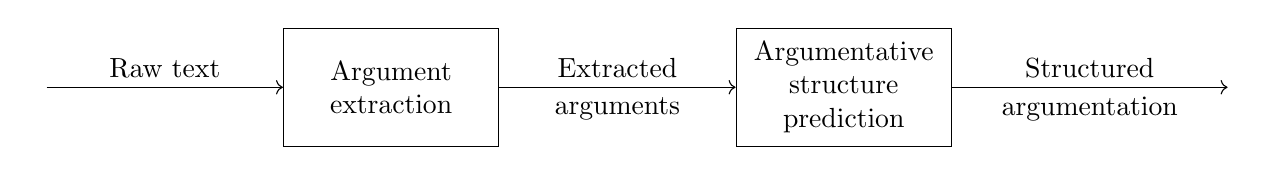
\begin{tikzpicture}
[box/.style={
rectangle, draw, text width=2.5cm, minimum height=1.5cm, align=center}
]
\node (most-left) {};
\node (argex) [box, right=3cm of most-left] {Argument extraction};
\node (argstruc) [box, right=3cm of argex] {Argumentative structure prediction}; 
\node (most-right) [right=3.5cm of argstruc] {};
\draw[->] (most-left) -- (argex) node [above, midway] {Raw text}; 
	\draw[->] (argstruc) -- (most-right) node [above, midway] {Structured} node [below, midway] {argumentation} ; 
	\draw[->] (argex) -- (argstruc) node [above, midway] {Extracted} node [below, midway] {arguments}; 
\end{tikzpicture}
	\caption{Pipeline architecture of an end-to-end argumentation mining 
	system}
	\label{fig:pipeline}
\end{figure}

\emph{Argumentation mining} is a discipline dealing with the automatic
identification and extraction of the structure of inference and reasoning
expressed as arguments presented in natural language
\citep{lawrence2019argument}.  Some refer to it as argument mining; we will use
both names interchangeably.  Argumentation mining combines elements of
\emph{natural language processing} (discussed briefly in
section~\ref{sec:natural_language_processing}) and \emph{knowledge
representation and reasoning} \citep{cabrio2018five}.  Typically, natural
language processing techniques are first used to extract arguments and
structure a debate or discussion. Then, once as the argumentative parts of a
debate or discussion have been extracted and structured, they are provided as
input to knowledge representation and reasoning systems.  Knowledge
representation and reasoning systems are usually in charge of providing various
argumentation analysis, examples being: determining prevailing stance,
detecting logical fallacies, or finding most frequently used claims.

To get from raw text to structured arguments a pipeline-like architecture
is usually employed (shown in figure~\ref{fig:pipeline}). 
Raw (natural language) text is input to an argument extraction module. This module
extracts elementary \textbf{argument components} from raw text. 
Once argument components are extracted, they are connected and structured 
according to some \textbf{argumentation model} (such as the Toulmin model \citep{toulmin2003uses}).
The output of the structuring module is usually some form of an argument graph. 
%An alternative, but similar architecture is shown
%in~\citep{lippi2016argumentation} where the argument extraction component 
%is elaborated further. 
In this thesis, we will mostly discuss extracting and structuring argumentative
portions of a textual debate. We will briefly showcase how a analysis can be
conducted in chapter~\ref{chap:analysis}. 

\subsection{Example}


Fig.~\ref{fig:example_pipeline} shows an example of an argumentation mining
pipeline. Two comments are taken from an online discussion forum on the topic
of ``\emph{Should marijuana be legalized?}''. The author of the first comment
is \con{against} the legalization of marijuana, the author of the second
comment is \pro{for} the legalization of marijuana.  In this example, we use an
argument model that defines argument components to be premises and conclusions.
Premises and conclusions are singled out in the first step of the pipeline.
The second step of the pipeline detects relationships between extracted
argument components and forms argumentation structures. In this case, the
argumentation structure is defined by the Freeman's model
\citep{freeman2011argument} which defines premises and conclusions with attack
or support relations amongst them. 

This example is from a dataset built by \citet{hasan2014you}. It demonstrates
some of the challenges of argumentation mining (and natural language processing
in general): the text contains typos (``\emph{nonsence}''), idiomatic
expressions (``\emph{because Marijuana is the drugs}''), requires solving
anaphora resolution to clarify context (``\emph{If you legalized, you could tax
it too}''), etc. All of these issues indicate that creating a coherent
argumentative logical structure from raw text is an extremely challenging
problem.

\begin{figure}[t!]
	\centering
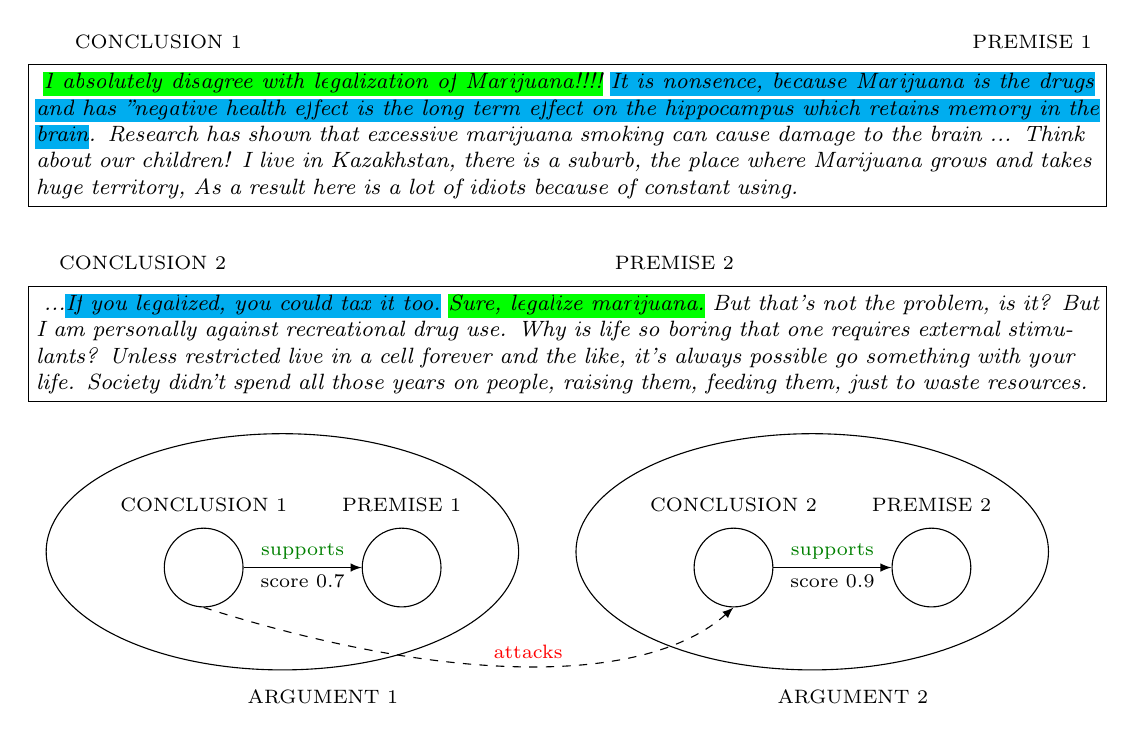
\begin{tikzpicture}
[
textbox/.style={rectangle, draw, text width=13.5cm, align=left, 
	},
arg/.style={circle, draw, minimum size=1cm}
]
	\footnotesize{
	\node (text1) [textbox] {
\emph{
	\hlgreen{I absolutely disagree with legalization of Marijuana!!!!}
	\hlcyan{It is nonsence,
	because Marijuana is the drugs and has "negative health effect is the
	long term effect on the hippocampus which retains memory in the brain}.
Research has shown that excessive marijuana smoking can cause damage to
the brain ...  Think about our children! I live in Kazakhstan, there is
a suburb, the place where Marijuana grows and takes huge territory, As
a result here is a lot of idiots because of constant using.
}
};
\node (text2) [textbox, below=1 cm of text1] {
\emph{
	...\hlcyan{If you legalized, you could tax it too.} \hlgreen{Sure,
	legalize marijuana.} But that's not the problem, is
	it? But I am personally against recreational drug use.
	Why is life so boring that one requires external stimulants?
	Unless restricted live in a cell forever and the like, it's always
	possible go something with your life. Society didn't spend all
	those years on people, raising them, feeding them, just to waste
	resources.
}
};
}
	\scriptsize{
	\node (conclusion1) [above right=0.1cm and 0.5cm of text1.north west] {CONCLUSION 1};
	\node (premise1) [above left=0.1cm and 0.1cm of text1.north east] {PREMISE 1};
	\node (conclusion2) [above right=0.1cm and 0.3cm of text2.north west] {CONCLUSION 2};
	\node (premise2) [above right=0.1cm and 0.5cm of text2.north] {PREMISE 2};
	}

	\node (invisible) [below=2cm of text2.south] {};
	\node (support1) [arg, left=1.5cm of invisible] {};
	\node (claim2) [arg, right=1.5cm of invisible] {};
	\node (claim1) [arg, left=1.5cm of support1] {};
	\node (support2) [arg, right=1.5cm of claim2] {};

	\scriptsize{
	\node (conclusion1) [above=0.1cm of claim1] {CONCLUSION 1};
	\node (premise1) [above=0.1cm of support1] {PREMISE 1};
	\node (conclusion2) [above=0.1cm of claim2] {CONCLUSION 2};
	\node (premise2) [above=0.1cm of support2] {PREMISE 2};

	\draw[-latex]  (claim1) -- (support1) 
	node [above, midway] {\textcolor{darkgreen}{supports}} node [below, midway] {score $0.7$} ; 

	\draw[-latex]  (claim2) -- (support2) 
	node [above, midway] {\textcolor{darkgreen}{supports}} node [below, midway] {score $0.9$} ; 

	\draw[-latex, dashed] (claim1.south) .. 
	controls ($(invisible) + (-1.5cm, -1.5cm)$ ) and ($(invisible) + (1cm, -1.5cm)$ )
	.. node[above, sloped] {\textcolor{red}{attacks}} (claim2.south);
	

	\draw ($(claim1) + (1cm, 0.2cm)$ ) ellipse (3 cm and 1.5cm);
	\draw ($(claim2) + (1cm, 0.2cm)$ ) ellipse (3 cm and 1.5cm);

	\node (arg1) [below right=1.1cm and 0.1cm of claim1] {ARGUMENT 1};
	\node (arg2) [below right=1.1cm and 0.1cm of claim2] {ARGUMENT 2};
	}
	% connect them

\end{tikzpicture}
\caption{Example of two comments processed using an argumentation mining pipeline. 
	First, argument boundaries are determined for the \hlcyan{conclusions} and 
	\hlgreen{premises}. Then \textcolor{darkgreen}{support} and 
	\textcolor{red}{attack} relations are
	determined between conclusions and premises
	to form arguments.
	}
	\label{fig:example_pipeline}
\end{figure}

\subsection{History}

Argumentation has roots in dialectics and philosophy where it was a branch of
knowledge dedicated to the study and analysis of how assertions are proposed
and debated, and how conflicts between opposing opinions are resolved
\citep{bench2007argumentation}.  Argumentation has been an essential part of
numerous areas, such as logic, rhetoric, jurisprudence, and computer science. 
Argumentation in computer science started with 
the work of \citep{dung1995acceptability} who explored knowledge representation
of argumentation. \citet{dung1995acceptability} and subsequent work on argumentation
knowledge representation led to the development of 
the area now known as \emph{computational argumentation}. 

Computational argumentation studies three different types of models of argumentation:
rhetorical, dialogical, and monological \citep{bentahar2010taxonomy}. 
The two former highlight argumentation as a dynamic process: rhetorical models
put emphasis on the role of audience and persuasive intention; dialogical 
models describe the ways arguments are connected in a dialogical structure. 
The latter, monological models emphasize the structure of the argument itself, 
including the relations between different components of a given argument. 

Another dichotomy in computational argumentation is between 
\emph{abstract argumentation} and \emph{structured argumentation}, with
Dung as the main proponent of abstract argumentation \citep{dung1995acceptability,
bondarenko1997abstract}. In abstract argumentation, each argument is an
atomic entity without internal structure. Contrary to that, 
structured argumentation proposes some internal structure for each argument, 
described through some representation formalism or model. 
Argumentation mining typically follow the structured argumentation
school. In structured argumentation it is common to annotate text data according to
a defined (usually established on some argumentation theory) formalism which is
then followed by building models to automatically derive argumentation
structure directly from text. There are many approaches in structured
argumentation, therefore there is no universally accepted definition of a
structured argument.  An intuitive definition of an argument was given by
\citet{walton1998new} as a statement consisting of three parts: a set of
premises, a conclusion, and inference from premises to a conclusion. However,
some literature (this thesis included) will denote premises and conclusions to
be referred to as claims.  What types of links can be established between
premises and conclusions (claims in general) varies greatly across different
argumentation models \citep{lippi2016argumentation}.

Independently of the development of computational argumentation and argumentation
mining, the area of \emph{opinion mining} (also referred to as sentiment
analysis) has developed as part of computational linguistics especially in the
2000s. Opinion mining identifies the emotional tone of a body of text
\citep{pang2008opinion}.  It attempts to identify sentiment (positive, neutral,
or negative) and emotional state (happy, sad, angry, \dots) of the author of
the text.  Identifying opinions towards different (usually divisive) issues has
been researched as part of \emph{stance classification}
\citep{walker2012stance, hasan2013stance}.  Both sentiment analysis and stance
classification
are closely related to argumentation mining. In argumentation mining people
provide claims towards a topic. Their claims are usually backed up with arguments. These
arguments may contain subjective opinions (based on sentiment) and often result
in a final stance towards the topic of discussion (``\emph{gay marriages
should be allowed}''). In that light, argumentation mining often
(but not always) involves analyzing subjective opinion and stance. 

Argumentation mining started to become featured more prominently in the 2010s.
The work of \citet{teufel2009towards} is considered to be one of the first in
argumentation mining. They proposed argumentative zoning for scientific papers
in which they attempt to extract and structure argumentation on the paragraph
level.  \citet{palau2009argumentation} first started to work on a sentence
level, as they proposed an end-to-end solution to extract and structure
sentence-level arguments from legal texts. The development of machine learning
and natural language processing sparked further research and interest in
argumentation mining. Extensive research has then been conducted that mainly
adopted the \emph{structured argumentation} approach.

Within the scope of this thesis, we are interested in \emph{monological},
\emph{structured argumentation}.  We wish to analyze online discussions without
accounting for the dialogical component, but merely the content of the
discussion. Structured argumentation is also the focus of our interest, as we
wish to grasp the semantics of arguments and claims, instead of treating them
as atomic units. Our structured argumentation approach is reflected in the fact that 
we decompose argumentative content into tokens, working our
way up to argument components. 

%- argumentation mining (often denoted as argument mining) started to gain dominance in 
%2010
%2010, when some of the 
%first methods to mine \textit{arguments} from natural language appeared in
%\citep{teufel2009towards} where they propose argumentative zoning for 
% scientific papers and \citep{palau2009argumentation} proposed to extract 
% and structure  arguments from legal texts. \\
%- development of machine learning and natural language processing sparked
%further research in the field of argumentation mining \\
%- since 2014 to 2019., there have been six argumentation mining dedicated workshops 
%co-located with top conferences in  computational linguistics (such as ACL and NAACL) \\
%- further, two seminars in Dagstuhl have been organized \\
%- two tutorials on argument mining have been held \\

% - One other definiton of argumentation mining states that
% it is  ``the general task of analyzing
% discourse on the pragmatics level and applying a  certain  argumentation  theory
% to  model  and  automatically analyze  the  data  at  hand'' \citep{habernal2017argumentation} \\
% 
% - argumentation mining spurned from people dealing with computational argumentation
% to develop more end-to-end methods \\

\section{Problems}
\label{sec:problems}

Two elementary problems of argumentation mining are 
extracting argument components from text and producing argumentative structure
from either extracted argument components or directly from text
(shown in Fig.~\ref{fig:pipeline}). 
Extracting argumentative components and producing argumentative
structure both make various assumptions about the data and downstream
applications. 
Extracting argumentative components from text can be done on different levels:
the sentence or the paragraph level, whereas structuring arguments can use
Toulmin's or Freeman's model.
More specifically, problems in argumentation mining can
usually be specified by five dimensions \citep{lippi2016argumentation}: 
\begin{itemize}
\item \emph{granularity of input text}, 
\item \emph{genre of input text}, 
\item \emph{argument model}, 
\item \emph{granularity of output}, and
\item \emph{goal of analysis}.
\end{itemize}

\emph{Granularity of input text} indicates the detail at which arguments
are processed. Some process arguments at the paragraph level 
such as the work on argumentative zoning
\citep{teufel2009towards}. Most of current research defines
sentences as the minimal unit of argumentation,
whereas some authors explore the sub- and intra-sentence levels
to detect argument component boundaries.

\emph{Genre of the input text} is defined by the type of input data processed.
Usually, a single genre of documents is explored within an argumentation
pipeline, such as legal documents \citep{palau2009argumentation}, scientific
articles \citep{teufel2009towards}, or online discussion forums
\citep{hasan2014you, boltuzic2014back, habernal2017argumentation}.  In
\citep{budzynska2014towards} they show how dialogue-agnostic and
context-agnostic models perform poorly.  Similar performance is shown in
\citep{daxenberger2017essence} where they also attempt to design cross-genre
methods. Genre-specific research is explored more comprehensively in 
section~\ref{sec:applications}.

Argumentation is structured through different \emph{argument models}.  The
argumentation model usually defines a formalism of argument components and
relationships between argument components.  Specific argument models are
described in section~\ref{sec:area_arg_struc_pred}.

Similarly to the granularity of the input, the \emph{granularity of the output}
varies. The lowest possible granularity of output is a specific argument
component, such as claim, evidence or premise. Argument components form arguments
which are of more coarse granularity. Some even go beyond the level of arguments, 
and attempt to output \emph{argumentation schemes} \citep{feng2011classifying} which
define the interactions across arguments, making them even coarser than arguments. 

Finally, the \emph{goal of analysis} describes the motivation behind solving
the argumentation mining problem. For typical argumentation mining problems
this can be (argument, claim) extraction, (argument component type)
classification, or (argument relation) prediction. An analyst can then 
summarize the discussion using the extracted claims, detect logical fallacies
of the extracted argumentation structure, etc.

Within the scope of this thesis, we will work on paragraph, sentence, and
sub-sentence \emph{granularity of input text}, with the emphasis on
sub-sentence level. We will define claims on a sub- and intra-sentence level as
part of the claim segmentation problem (chapter~\ref{chap:claim_segmentation}).
The \emph{genre of input} will be, as the title suggests, online discussions.
We define our own \emph{argumentation model} in
chapter~\ref{chap:formalization} which is inspired by Freeman's model and the
work of \citet{hashimoto2012excitatory}.
The \emph{goal of analysis} of the thesis is claim extraction.
Next, we describe elementary problems of argumentation mining
argument component extraction and argumentative structuring 
in more detail.

% One example is the project of creating the
% Argument Web (argumentative Semantic Web) which defines knowledge
% representation standards for arguments compatible across different
% argumentation theories \citep{rahwan2007laying}. 

%- five dimensions of input are usually give: 
%granularity of input, genre of input, argument model, 
%granularity of target, goal of analysis \\
%- granularity of the processed text indicates  the detail at
%which arguments are processed \\
%- some consider argument processing at the level of paragraphs, 
%for example argument zoning \citep{teufel2009towards} \\
%- most of current research focuses on sentences, whereas some authors
%go to the intra-sentence level and detect argument component boundaries \\

% \noindent - the genre aspect defines the type of input data, such as legal/law, 
% online discussions, news, essays, etc. \\
% - existing approaches have mainly considered a single genre \\
% - for example, \citep{budzynska2014towards} shows how AM need
% context, a dialogue-agnostic models do not work \\

% \noindent - tasks of argumentation mining are 
% \begin{itemize}
% \item prominent claim identification,
% \item claim clustering,
% \item claim extraction,
% \item deriving implied claims.
% \end{itemize}
% 
% \noindent - Argument extraction -- first step in identification of arguments
% within the input natural language text \\
% - may be further split per component extraction (claim/premise extraction) and
% by identification of text boundaries \\
% 
% \noindent - Relation prediction -- predicting what are the relations holding 
% between the arguments identified \\
% - the relations may heteregeneous, such as \emph{attack} and \emph{support}\\
% - upon their identification, these relations are used to connect arguments to 
% graphs, in which relations connecting the retrieved arguments (nodes of the graph)
% correspond to the edges \\

% \section{Argument analysis}
% 
% \noindent - manual argument analysis \citep{lawrence2019argument}
% - manual analysis often involves using various tools to analyze arguments, 
% such as Araucaria \citep{reed2004araucaria}, OVA \citep{reed2014ova+}, or
% Carneades \citep{gordon2007carneades} \\
% - these tools require already extracted claims that the tool users can then 
% connect, determine their roles (premise, conclusion) and define 
% relationships (attack, support), and even form refined structured,
% such as argumentation schemes \citep{walton2008argumentation} \\
% Generally, steps to perform argument analysis are:
% \begin{itemize}
% \item text segmentation,
% \item argument / non-argument,
% \item simple structure,
% \item refined structure.
% \end{itemize}

\subsection{Argument component extraction}
\label{subsec:arg_comp_ext}

The first stage of argumentation mining is detecting argumentative parts from
raw text.  There exists no standard for an elementary unit of argumentation,
but the definition is usually shaped to tailor a specific need. In discourse and
rhetoric theory, the basic element of an argument is called an \textit{Elementary
Discourse Unit} EDU. EDUs are defined as clauses \citep{winter1982towards,
givon1983topic}, sentences \citep{polanyi1996linguistic}, or 
prosodic units \citep{sacks1978simplest}. All these approaches agree an EDU
should be a non-overlapping atomic unit of text. Another strand of research defines
an \textit{Argumentative Discourse Unit} (ADU) as a minimal unit of discourse
\citep{peldszus2013argument} which can be composed of multiple EDUs, but ADUs
can overlap. As \citep{lawrence2019argument} points out, there are multiple
issues with with defining the rules to constitute an argument building block.
In the scope of this thesis, we will use the term \emph{argument
component}, and define argument components as a generalization of
an EDU, an ADU, and more specific argument elements (such as claims).
There are two dominant approaches to argument component extraction:
\begin{enumerate*}[label=(\arabic*)]
		\item sentence-level detection and
		\item argumentative boundary detection.
\end{enumerate*}

Sentence-level detection is typically performed by taking an input text, 
splitting it by sentence, and then classifying each sentence as
argumentative or non-argumentative based on its (and surrounding) content. 
Argument boundary detection is usually performed on a token level
to extract argumentative parts that constitute argument components
\citep{lippi2016argumentation}.

\paragraph{Sentence-level detection.} 
In practice, sentence-level detection is commonly achieved through one of three
setups by either using:
\begin{enumerate}
\item a binary classifier trained to distinguish argumentative from 
	non-argumentative sentences, leaving the task of identifying component type
	(claim, premise, \dots) to some other system, 
\item a multi-class classifier trained to discriminate all argument components that
	exist in the adopted argument model; this assumes a sentence can contain at most
	one argument component, or 
\item a set of binary classifiers; one for each existing argument component in
	the considered model, so that a sentence can be predicted to contain
		more than one argument component (conceptually, as this is
		multi-label classification, it could be achieved using any
		viable multi-label classification method, some described in 
		section~\ref{sec:chain_classification}).
\end{enumerate}
Different classification tools have been employed,  
some of them being Logistic Regression, Maximum Entropy, Decision
Trees, Random Forests, Support Vector Machines (described in section~\ref{sec:svm}).
See \citep{lippi2016argumentation} for a comprehensive list of methods used for 
sentence-level argument component detection.
There is no clear evidence to conclude which classifier works best 
in which situation, mostly since different classifiers have been applied
to different datasets. 

The input for classifiers is based on features, which were mostly built from
input text.  A lot of effort has been produced in hand-crafting significant
features to solve the argument component extraction problem.  The most commonly
used feature sets are bag-of-words BoW (described in section~\ref{sec:bow}) and
\emph{tf-idf} (described in section~\ref{sec:tf-idf}). Other features rely on
third-party grammatical information, such as constituency and dependency parser
outputs. These provide features like part-of-speech (POS) tags
\citep{manning2011part} which describe the token role in a sentence (noun,
verb, adjective, etc.).
Some features have been designed specifically for dataset in hand, such as verb
tense information \citep{palau2009argumentation, stab2014identifying}, or
discourse markers \citep{eckle2015role}. Lately, more sophisticated semantic
features are used,
such as subjectivity scores, sentiment detectors, or named entities \citep{levy2014context}.  
Since the argument component
extraction can be heavily domain dependent, \citet{palau2009argumentation} have
compiled a list of syntactic indicators that are very frequent in judicial
language which provide reliable cues to detect structural patterns. Similarly,
in \citep{levy2014context, rinott2015show} they show that providing topic
information when extracting argumentative components is helpful. Providing domain
specific information is called \emph{context dependent detection}. On the other
hand, \citep{lippi2015context} attempt to develop develop \emph{context independent
detection} methods and features. They exploit structured kernels based on
constituency parse trees to capture the rhetorical structure of a sentence. 

\paragraph{Argumentative boundary detection.} Determining the exact boundary of
each argumentative component is an alternative to sentence detection. It allows
for a more fine grained (usually token-level) approach, as using sentences
might not fit the argumentation structure (or definition of the elementary
argument component).  The problem in argumentative boundary detection is
determining where each argument component starts and ends.
Relating to the sentence-level detection, there are 
multiple things to consider:
\begin{itemize}
\item An argument component can map exactly to a sentence;
\item Two or more argument components can be in a single sentence (and potentially overlap);
\item An argument component can span across multiple sentences;
\end{itemize}
In sentence level detection, mapping exactly to a sentence is always assumed
\citep{palau2009argumentation, levy2014context}. 
In \citet{habernal2014argumentation} annotation study they report
that the average claim (argument component) spans 1.1 sentences and an average
premise spans 2.2 sentences on a sample size of ${\sim}4,000$ sentences 
indicating that a single argument component 
rarely maps to a single sentence. In the IBM dataset \citep{levy2014context},
they discern between different argument components: claims are short texts
contained within a sentence, while premises can span multiple sentences. But, when
determining boundaries, they allow consecutive segments to span up to three
sentences within a paragraph \citep{rinott2015show}.
In many works, the boundary detection is skipped altogether as it assumed to have
been done independently \citep{stab2014identifying, eckle2015role}. 

Determining argumentative boundaries at a token level can be modelled as a
sequence labeling. In sequence labelling problems, each token is assigned a
label indicating whether it belongs to an argumentative component or not.
Then, usually structured prediction approaches are deployed in order to take
advantage of cross-label
dependencies and provide the most likely sequence of labels
(more on structured prediction approaches to sequences
in sections~\ref{sec:crf}, and~\ref{sec:hmm}).  In argumentation mining, this
approach has been used in \citep{goudas2014argument, sardianos2015argument,
park2015conditional}.  They use conditional random fields to segment boundaries
of argument components.  We will use a similar approach in
chapter~\ref{chap:claim_segmentation} for claim segmentation. 

%This can be done on a sub-sentence level \citep{habernal2014argumentation}. 

% TODO clarification of our level of claims does not need to be here
% - to overcome this, we therefore, define \textit{claims} to allow
% for overlapping and don't define them in terms of phoentics or sytnax, but
% state they should be semantically atomic \\ 
% - an example why we allow overlapping claims: \\
% \begin{mydef}
% The church stated that people should not perform abortion or 
% smoke marijuana. 
% \end{mydef} 
% - as text segments \textit{the church stated that people should not perform
% abortion} and \textit{the church stated that people should not smoke marijuana}
% both convey atomic thought, we feel it would be wrong to make this a single 
% claim \\
% - on the other hand, having it two claims, but omitting \textit{the church stated}
% in one claim, but not the other makes a claim completely different as
% context is lost \\
% - we also don't wish to rely on text containing subjects or predictes as 
% texts in online discusses are often times ungrammatical \\
% - this means that we consider that utterances
% \textit{Yes, definitely!} and \textit{Marijuana should definitely be allowed}
% can both claims of the same meaning, given the context they are made in. \\

\subsection{Argument structure prediction}
\label{sec:area_arg_struc_pred}

Argument structure prediction structures extracted argument components
according to an \emph{argument model} and a desired \emph{granularity of
output}. It usually involves predicting relations and connections of pairs of
argument components. The output is a graph connecting the retrieved argument
components, where nodes and edges represent argument components and relations
between argument components respectively. Edges may represent different
relations, such as entailment, support, or conflict
\citep{lippi2016argumentation}. An argument graph can then be used
for various applications: social network analysis, acceptance of different
arguments (often studied as part of computational argumentation), studying
persuasive rhetorical strategies, etc.

\paragraph{Argument model. } The two most popular argument models are the 
Toulmin's \citep{toulmin2003uses} and Freeman's \citep{freeman2011argument} model. 
\citet{toulmin2003uses} proposed a model structure of human argumentation that
consists of six core elements: claim, evidence (grounds, datum), warrant,
qualifier, rebuttal, and backing.  Out of these six, every argument must
contain three fundamental parts: claim, evidence, and warrant. A \emph{claim}
is the assertion that the author of the argument would like to prove to their
audience. \emph{Evidence} is the basis on which the claim was made, and the
\emph{warrant} serves as the rule of inference that links the evidence to the
claim. The \emph{qualifier} indicates the certainty of the claim, and the
\emph{rebuttal} is an acknowledgement of an alternative valid view towards the
claim.  The Toulmin model is used in law, design, policy making, science,
philosophy, etc.  
Argument components of Freeman's model are claims
and premises.  Claims and premises are connected using support or attack
relations.  The claim/premise model is adopted by most research on
argumentation mining \citep{palau2009argumentation, peldszus2013argument,
stab2014identifying, eckle2015role}.  \citep{stab2014identifying,
biran2011identifying} both adopt Freeman's model and employ a binary SVM
classifier to predict links between claims and premises.
\citet{boltuzic2014back} adopt an expanded Freeman's model to try several
different setups to predict relations (support/attack/neutral) between claims
(described in more detail in chapter~\ref{chap:argrec}).  In
\citep{stab2014annotating, liebeck2016airport} they adopt a modified Freeman's
model where they discern between major positions, claims, and premises. 
\citet{liebeck2016airport} relate their argument model
to both Freeman's and Toulmin's model. In contrast to the simple
Freeman's model, adopting the Toulmin model induces more sophisticated argument
structure prediction. All the components of the Toulmin model (claim, data,
warrant, qualifier, rebuttal) have to be identified correctly in order to
retrieve the correct final structure.  In \citep{habernal2014argumentation}
they annotate a dataset according to the Toulmin model and build models to
predict elements of the Toulmin model.  Additionally, in
\citep{habernal2014argumentation} they list different different argument models
used across argumentation mining research.

% \paragraph{Output granularity. }
% Producing a Toulmin model 

Current approaches to argument structure prediction make several simplifying
hypotheses. In \citep{aharoni2014benchmark} they always associate the evidence
with the claim (which might not be the case in practice).
\citet{palau2009argumentation} build a context-free grammar that is genre
specific to predict relations between argument components. The grammar follows
rhetorical and structural patterns observed in legal documents, thus it is
highly unlikely this grammar would generalize to other genres. 

\section{Applications and Corpora}
\label{sec:applications}

Argumentation mining has been researched with a specific application in mind.
Conducted research has been designed to help education, law, politics, decision
making and other many other areas. 

\paragraph{Education.} In education, the goal may be to improve critical
thinking skills.  Argumentation mining has been used to analyze documents to
automatically output the argumentation structure from documents.  Persuasive
essays have often been the object of analysis. In a persuasive essay, the
author attempts to persuade the audience (readers) that the authors' point of
view is the most informed, logical and has valid perspective on the topic
\citep{cabrio2018five}.  \citet{stab2017parsing} build a corpus of persuasive
essays and propose an approach to identify argument components
using sequence labelling methods operating at the token level. They also design
a joint model for detecting argumentation structures (additionally optimized
using integer linear programming constraints). In \citep{eger2017neural} they
use the aforementioned corpus and go a step further to propose an end-to-end
argumentation mining system to get from raw text to argumentation structures.
Similarly, \citet{nguyen2018argument} implement an end-to-end system on
persuasive essays, but their end product is argumentative features they deem
valuable for other argumentation mining tasks. \citet{peldszus2015joint}
create another corpus of English-German essays microtexts\footnote{Corpus of
English-German microtexts available at
\url{https://github.com/peldszus/arg-microtexts}}. They jointly predict
different aspects of argumentation structure by combining different sub-task
prediction and create an evidence graph. On the evidence graph they apply the
Minimum Spanning Tree decoding algorithm \citep{raidl2000weighted}.  They
borrow from Freeman's dialectical theory by using moves of the proponent and
challenger to model argumentation structure.

\paragraph{Wikipedia.} IBM has funded argumentation research projects that are
dedicated to Wikipedia data. \citet{levy2014context} introduce a dataset based
on Wikipedia on which they perform the task of automatically detecting
\emph{context dependent claims} CDC.  They define a CDC as a concise statement
that directly supports or contests the given topic discussed in the debate. As
a follow up, \citet{rinott2015show} attempt to automatically detect evidence of
a given claim from Wikipedia.  They call this \emph{context dependent evidence
detection}.  The continue their work in \citep{bar2017stance} where they
perform stance classification by decomposing it into the detection of: 
\begin{enumerate*}[label=(\arabic*)]
	\item targets given the topic and the claim,
	\item the polarity of a text segment towards each detected target, and
	\item whether the targets are contrastive or consistent. 
\end{enumerate*}
Enriching the dataset made by \citet{levy2014context}, \citet{bar2017stance}
introduce \pro{pro} / \con{con} stance labels. This dataset is then experimented on in
\citep{lippi2016margot}, where the MARGOT (Mining ARGuments frOm Text) system
does argument component classification and boundary detection. 

\paragraph{Online discussions and web debating platforms.}
There is an abundance of online resources which could be used for
massive argumentation analysis on various controversial topics, such as 
``\emph{abortion}'' or ``\emph{euthanasia}''.
\citet{habernal2017argumentation} mined and annotated user-generated
Web discourse (following a modified Toulmin's model) and propose 
a sequence labelling approach to identify argument components. 
In \citep{niculae2017argument} they propose a structured prediction approach 
for argumentation mining (comparing SVN and RNN algorithms) that jointly
learns to classify elementary argumentative units and identify argumentative relations
between elementary argumentative units on Cornell eRulemaking Corpus\footnote{Corpus 
available at \url{https://facultystaff.richmond.edu/~jpark/data/jpark_lrec18.zip}}
and the persuasive essay corpus \citep{stab2017parsing}.
\citet{cabrio2012combining} use data from an online debating platform
Debatepedia\footnote{available on \url{idebate.org}} and tackle the relation 
prediction task using textual entailment. 
In \citep{al2016cross} they create a large corpus annotated with argumentative
text segments (also from Debatepedia) and create a binary classifier to determine
whether text is argumentative or not. \citet{dusmanu2017argument} collect 
a Dataset of ARgumentative Tweets (DART) and build models to distinguish argumentative
vs. non-argumentative tweets on topics ranging from Brexit and Grexit to 
the release of the new Apple Watch. 
\citet{habernal2016argument} study internet resources and 
focuses on argument persuasion to study when
an argument in more convincing than another argument. 

\paragraph{Legal documents. } 
In the legal domain, argumentation mining has been used to detect
premises, claims, and argumentation schemes to simplify
the work of judges and law scholars in identifying similarities 
across different judicial procedures. 
\citet{palau2009argumentation} propose a system that detects argument components, 
and predicts inter-argument relations. They first define a context-free
grammar, then use statistical classifiers to predict relations among different 
argument components. They work on the European Court of Human Rights (ECHR) Corpus.
\citet{teruel2018increasing} presents a new ECHR corpus with annotated 
premises, claims, and attack or support relations amongst them.
\citet{grabmair2015introducing} work on the U.S. Court of Federal Claims
cases and attempt to aid the decision of whether the compensation claim
complies with the federal statute from the National Vaccine Injury Compensation
Program. They propose a legal UIMA-based \citep{ferrucci2004uima} system 
that extracts argument-related semantic information from legal documents: clauses,
evidence-based facts, evidence-based reasoning, and other. 

\paragraph{Political speeches. }
The political domain allows for intuitive applications of argumentation mining. 
One can try to detect argumentation fallacies, measure persuasiveness of speeches, or
coherence of politicians' arguments. 
In \citep{lippi2016argument} they analyze political speeches from the 2015
UK parliamentary elections where they perform claim detection. 
They study vocabulary-based features and their impact to claim detection. 
\citet{walker2012corpus} create the Internet Argument Corpus (IAC) using
data from \emph{4forums.com}, a website for political debate, and use it
in subsequent work \citep{walker2012stance, abbott2016internet}. 
The posts from the forum are annotated with argumentative markers, such
as agreement with the previous post, cordiality, audience direction, 
assertiveness, emotionality, and sarcasm. 
\citet{duthie2016mining} apply argumentation mining to detect the presence and polarity 
of ethotic arguments from UK parliamentary debates, and visualize their results. 
\citet{naderi2015argumentation}  show how features based on embedding representations 
can improve discovering various frames in argumentative political speeches.
They propose a corpus of speeches from Canadian Parliament, and examine statements 
with respect to the position of the speaker towards the discussed topic
(\pro{pro}, \con{con}, no stance).
\citet{menini2018never} address the problem of relation prediction on 
political speeches in monological form (no interaction between opponents).
They create a corpus based on the transcription of speeches and official declarations 
issued by Nixon and Kennedy during 1960 Presidential campaign.

\paragraph{Other applications. } Most of argumentation mining
applications listed so far have followed 
the pipeline outlined in Fig.~\ref{fig:pipeline}. 
Some other studies related to argumentation mining have tried to gain 
some general insights related to argumentation (regardless of genre or application). 
\citet{habernal2016argument} focused on argument persuasion and studied
when an argument is more convincing than another. 
\citet{rosenthal2012detecting} tried detecting assertions containing some belief
of whose truth a user attempts to persuade the audience.
Whether claims and evidence are verifiable or not was studied by
\citep{park2014identifying, park2015conditional}.
\citet{ong2014ontology} built an argumentation structure using an ontology to
predict essay scores. 
Studying implicit argument components, such as implicit premises and implicit
warrants is also of interest in argumentation mining, as additional
implications may be derived. Recognizing implicit premises was studied in
\citep{park2015conditional, boltuzic2016fill} \citet{habernal2017argument}
organized a SemEval 2018 competition \emph{Argument Reasoning Comprehension} to
find implicit warrants between a claim and a premise.  More on recognizing
implicit claims will be mentioned in chapters~\ref{chap:deriving_implicit}
and~\ref{chap:analysis}.

%\paragraph{Other.} 
%Some less explored applications of argumentation can be found in 
%areas such as 
%medical decision support, multi-agent systems, and engineering, 
%policy decision making \citep{tremblay2016value, byron2019evaluating}.

%\noindent - newer applications and research in argumentation mining \\
%- \citep{habernal2016argument} focused on argument persuasion to study 
%that an argument is more convincing than another \\
%- argumentation mining is strongly connected to areas where 
%fact checking, misinformation, explanation of machine decisions \\
%- other areas as medicine (information upon randomized clinical trials),
%politics (identify fallacies and unfair propaganda), cyberbully prevention
%(attacks against a person)
%\citep{cabrio2018five} \\

\section{Discussion}
\label{sec:area_discussion}

Even though it is an emerging and popular area, there has been criticism
towards argumentation mining.  Performance of argumentation mining systems is
generally too low for practical application. Low performance can be partially
attributed to a generally low agreement rate observed in dataset annotation
\citep{peldszus2015joint, boltuzic2017toward}. This indicates that annotating
arguments is considered difficult even for humans. Additionally, there is a lot
of heterogeneity across different datasets. Each dataset is annotated according
to different annotation guidelines and nomenclature which is usually
inconsistent across datasets.  \citet{daxenberger2017essence} attempted to work
across six different argumentation mining datasets to determine the corpus
independent essence of a claim.  They conclude that consistency of the claims
still needs improvement.  \citet{wachsmuth2017argumentation} studied how
different theoretical models and practical views of arguments are, as they
showed how little differences in argumentation theories are shown in annotated
argument data.  However, there do exist some practical applications of
argumentation mining, such as the argument search engine \emph{args}
\citep{wachsmuth2017building}.

In this thesis, we work with monological, structured argumentation set in the
online discussion genre.  We set no specific practical application as a goal,
but wish to explore general insights in argumentation in online discussions. 
Understanding what are the most frequent claims and how are they 
stated, as well as deriving implicit thoughts and opinions from text 
are examples of insights we hope to uncover. 


\chapter{Methods and Tools for Argumentation Mining of Claims}

%This chapter is divided into three main parts. 
This chapter should be viewed as an overview of most methods used in the rest
of the thesis. Models of argumentation mining are mostly built on machine
learning, which is introduced in section~\ref{sec:unstruc_machine_learning}.
Then, in section~\ref{sec:struc_machine_learning} we focus on a
subarea of machine learning, structured prediction, as it is the foundation of
part~\ref{part:struc}. Next, as argumentation mining is a subarea of 
natural language processing, a brief introduction to the field, along with some
relevant problems will be explained in section~\ref{sec:natural_language_processing}. 
Finally, knowledge represetation relevant to this thesis will be explained in
~\ref{sec:knowledge_representation}. 

\section{Machine Learning}
\label{sec:unstruc_machine_learning}

- machine learning algorithms learn from data \\
- two basic purposes: supervised and unsupervised algorithms \\
- supervised algorithms fit a set of $n$ samples of 
input data $\textbf{X}^n \in \mathbb{R}^n$ to the set of their correponding 
labels $y^n $. When the labels are discrete $y \in \{1, 2, \dots , V\}$ 
supervised learning is called classification (of $V$ classes), 
whereas learning to fit continuous values ($y \in \mathbb{R}$) 
is denoted regression \\

\subsection{Support Vector Machines}
\label{sec:svm}

Support Vector Machines (SVM) \citep{cortes1995support} is one of the most
popular machine learning algorithms. The algorithm has proven useful for many
text-based problems, such as spam classification \citep{drucker1999support},
sentiment analysis \citep{wang2012baselines}, text categorization
\citep{joachims1998text}, and text classification in general
\citep{tong2001support, ikonomakis2005text}. Originally designed as a simple
binary classification procedure, it has been extended to support multiclass
classification \citep{weston1998multi}, structured prediction
\citep{tsochantaridis2005large}, weighted learning \citep{huang2005weighted} and
other. 

Consider a binary classification problem where one has
a training set $S$ consisting of $N$ pairs of examples with assigned labels
$(x_i, y_i)$.

$$
S = \{(x_1, y_1), (x_2, y_2), \dots, (x_N, y_N)\}
$$
where $\forall i, x_i \in \mathbb{R}^d, y_i \in {0, 1}$.
The SVM algorithm first projects the input data $x_i$ to 
higher dimensional space using a 
feature transform function $\phi(x_i)$ then attempts to 
find support vectors which are solutions to the equations:
\begin{align*}
\textbf{w}^T \phi(X) + b = -1 \\
\textbf{w}^T \phi(X) + b = 1
\end{align*}

The solutions to the equations represent margins which divide
the two classes ${-1, 1}$.
The margin width is $\frac{2}{||w||}$. 
To find the weights, one needs to 
optimize for two criteria 
\begin{enumerate*}[label=(\arabic*)]
\item maximize margin width and
\item minimize classification loss
\end{enumerate*} which is done by
$$
\min_{\textbf{w}} \left( \frac{1}{2}||\textbf{w}||^2 + C \sum_{i=1}^{N} \xi_i \right)
$$
where $\xi_i$ is the loss function and $C$ is a parameter of the model.
Typically, \textit{hinge loss} is used as the loss function $\xi_i(x_i, y_i) =
\max(0, 1 - y_i(\textbf{w}^T x_i + b))$ This problem can be solved using
various methods, such as quadratic programming \citep{wu2005svm} or stochastic
optimization \citep{wang2012breaking}.


\subsection{Long short-term memory networks}
\label{sec:lstm}

\begin{figure}
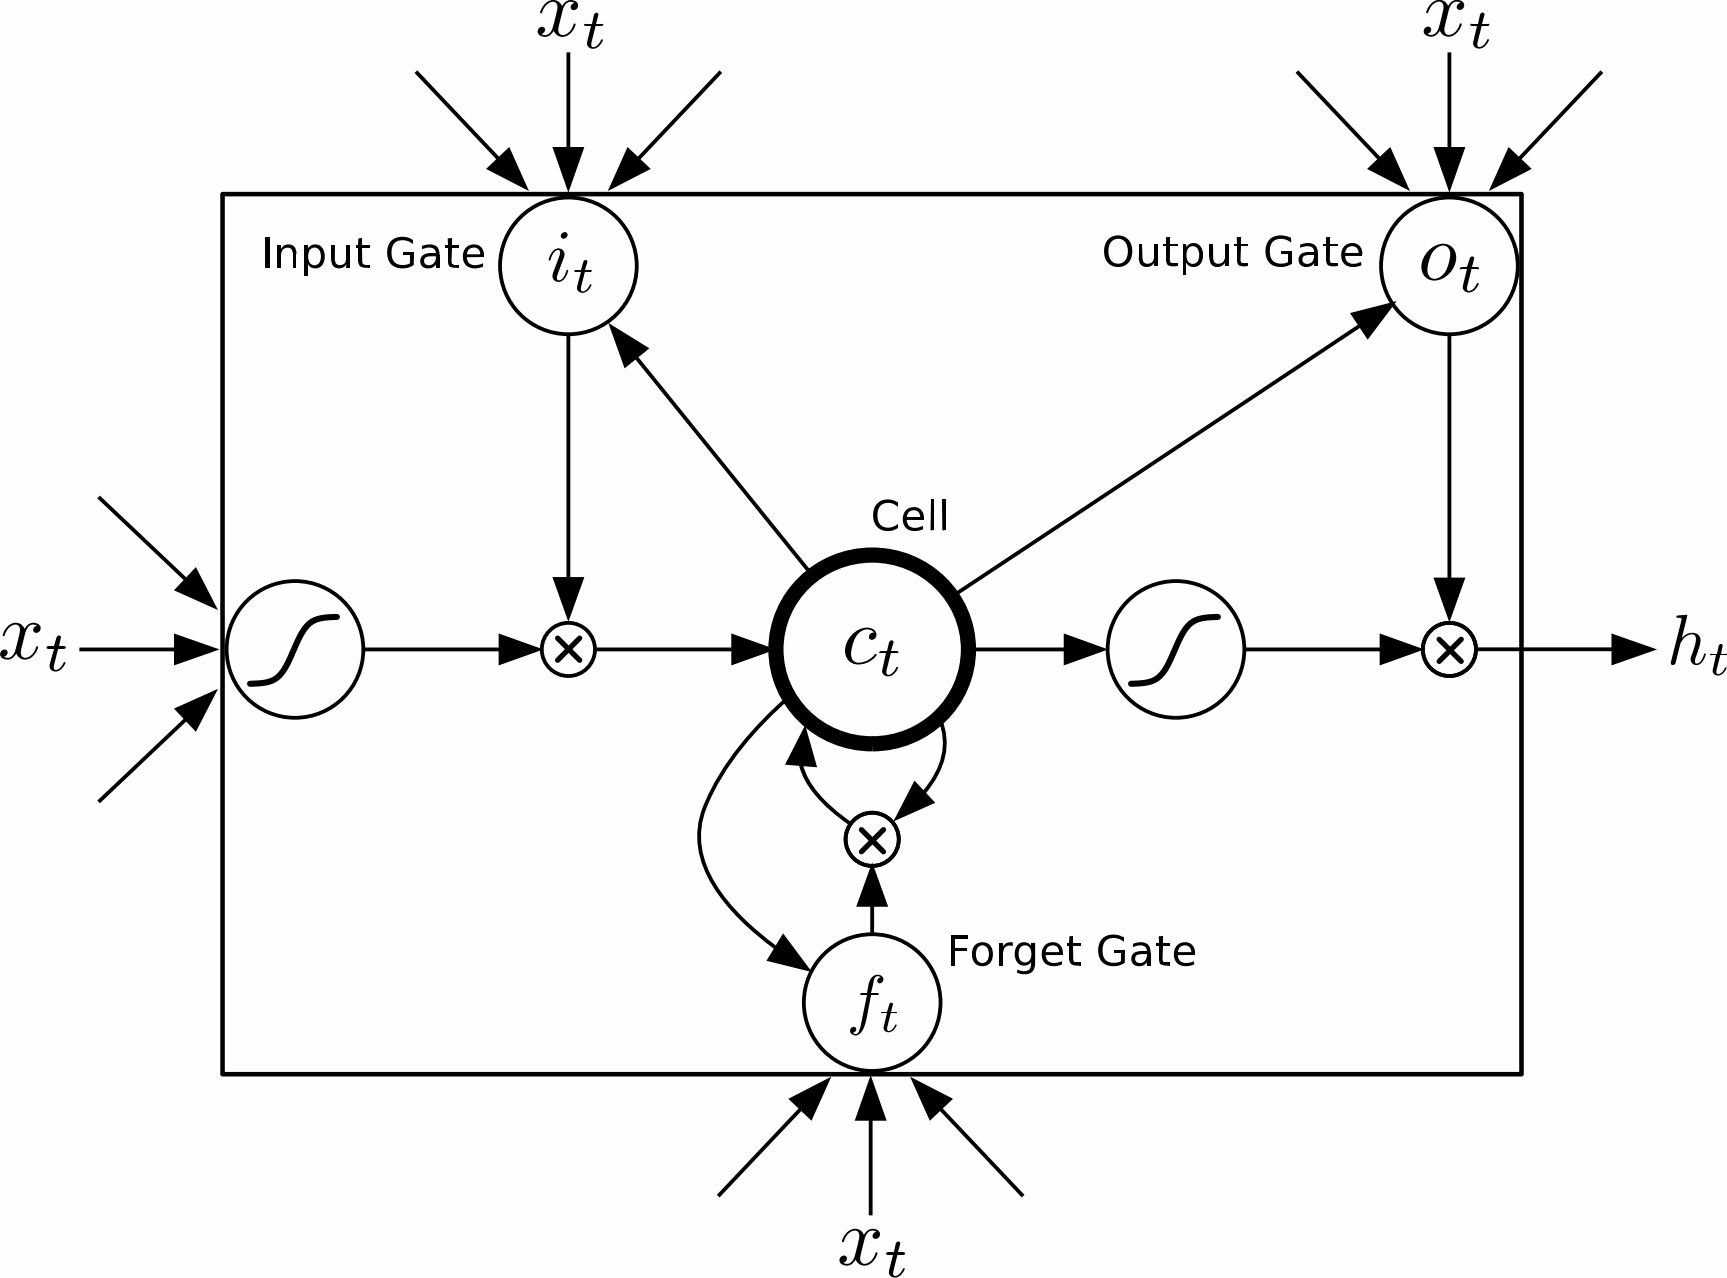
\includegraphics[scale=0.23]{lstm_2.png}
\caption{Long short-term memory network cell diagram. The cell consists of the 
	cell, input gate, forget gate and output gate. The LSTM receives
	the hidden state at the previous time step ($h_{t - 1}$) and $x_t$
	and outputs the hidden state $h_{t}$
	Adopted from 
\citep{graves2013hybrid} }
\label{fig:lstm_arch}
\end{figure}

Long short-term memory (LSTM) is an recurrent neural network
designed to process sequences of data 
\citep{gers1999learning}. A unit of LSTM consists of 
a cell, an input gate, an output gate and a forget gate.
The cell stores information over time intervals and the
gates control which data will be passed on the cell 
or not. Figure \ref{fig:lstm_arch} shows an LSTM cell. 
The input gate ($i$, which new information is going to be stored), 
forget gate ($f$, which information is going to be forgotten from 
the cell state), and output gate ($o$, which is the final output 
of the block) 
are calculated (at timestep $t$) from the input ($\mathbf{x_t}$) and 
previously calculated hidden state ($\mathbf{h_{t-1}}$):
\begin{align*}
	\mathbf{i_t} &= \sigma(\mathbf{w_i} [\mathbf{x_t}, \mathbf{h_{t - 1}}] + b_i) \\
	\mathbf{f_t} &= \sigma(\mathbf{w_f} [\mathbf{x_t}, \mathbf{h_{t - 1}}] + b_f) \\
	\mathbf{o_t} &= \sigma(\mathbf{w_o} [\mathbf{x_t}, \mathbf{h_{t - 1}}] + b_o) \\
\end{align*}
where $\mathbf{w_i, w_f, w_o}$ and $\mathbf{b_i, b_f, b_o}$
are learnable weights of the network and $\sigma$ is the 
sigmoid function ($\sigma(x) = 1 / (1 + e^{-x})$). Next, the 
cell state ($c_t$) and next hidden state ($h_t$) can be calculated as:
\begin{align*}
	\mathbf{\hat{c_t}} &= tanh(\mathbf{w_c} [\mathbf{x_t}, \mathbf{h_{t - 1}}] + b_c) \\
	\mathbf{c_t} &= \mathbf{f_t} \cdot \mathbf{c_{t - 1}} + \mathbf{i_t} \cdot \mathbf{\hat{c_t}} \\
	\mathbf{h_t} &= \mathbf{o_t} \cdot tanh(\mathbf{c_t}) \\
\end{align*}
where $tanh$ represents the hyperbolic tangent function.


The advantage over regular recurrent neural networks, which
don't posses any gating mechanism, is to stop the 
vanishing \citep{hochreiter1998vanishing}
and exploding gradient problems \citep{pascanu2012understanding}. 
The gradients from backpropagation 
can either vanish or explode when training
neural networks causing weight changes to either
stop (vanish) or take on extreme values (explode).
LSTM networks have been successfully applied to a number of problems,
such as language modeling 
\citep{sundermeyer2012lstm}, 
text classification 
\citep{zhou2015c}, question answering 
\citep{zhu2016visual7w}, machine translation
\citep{luong2014addressing}, and many more. LSTM networks are widely considered 
to provide a strong baseline for 
text-based problems. There exist many variations of LSTM networks, 
one example being gated recurrent units (GRU) \citep{chung2014empirical}.

% \subsection{Model Validation}
% 
% Machine learning models are evaluated on unseen data
% to estimate their performance. Traning and testing on the same
% data would lead to overfitting, meaning the model would
% not be able to generalize on new data. 
% To prevent that, 
% data is organized such that 
%  models aren't trained on data they are evaluated on
% (section~\ref{sec:selection})
% after which models are evaluated on unseen data by 
% comparing model predictions versus correct (gold) data
% through various metrics (section ~\ref{sec:metrics})

\subsection{Model Selection}
\label{sec:selection}

The basic model selection method is \textit{holdout}. 
In holdout, the dataset is randomly partitioned into three 
samples: training set (used to train the model), 
validation set (used to assses model performance during training),
and test set (used to asses model performance after training). 

\begin{figure}
	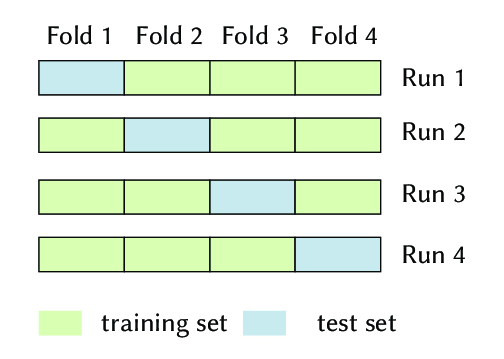
\includegraphics[scale=0.7]{kfold.png}
	\caption{
		Illustration of partitioning a dataset using k-fold model 
	selection using $k = 4$. In each case, $k - 1$ folds
	are used for the training set (green), and the remaining fold is
	the test set (blue). Adopted from \citep{pedregosa2015feature}}
	\label{fig:kfold}
\end{figure}

Another technique to partition datasets into training and test datasets
is cross validation \citep{arlot2010survey} (illustrated in~\ref{fig:kfold})
The training dataset is then used to train the model, and the remaining
test dataset is used to evaluate the resulted trained model. 
\textit{K-fold} cross-validation is the most commonly used
cross-validation technique in which the dataset is partitioned into 
$k$ equally sized samples called folds. One of the $k$ folds is
used as a test dataset, the rest comprise the training dataset. This
procedure is repeated $k$ times (usually $k \in [4, 10] \cap k \in Z$).
Using this method each dataset instance is in the test set 
exactly once. 

In addition to partitioning the data, model selection often involves finding
the optimal hyperparameters of the model, which involves  training and
evaluating the model with a different set of hyperparameters.  Exhaustively
searching through all possible combinations of hyperparameters is called
\textit{grid search} \citep{bergstra2012random}. There are some more advanced
techniques such as \textit{Bayesian optimization}.  For an overview of
hyperparameter optimization techniques see \citep{snoek2012practical}.

\subsection{Evaluation Metrics}
\label{sec:metrics}

Machine learning models are evaluted using metrics to quantify
performance. Supervised classification is more straightforward 
to evaluate and is usually evaluated by calculating  
precision, recall, and f-score. 

In a binary classification setting, we compare bit vectors ($1$ represents the
positive class) of predicted and gold labels. Element-wise comparison will
always give one of four combinations in a confusion matrix (shown in
table~\ref{tab:conf_mat}). Accuracy, precision, recall, and fscore between 
a gold vector $\mathbf{a} = (a_0, a_1, \dots, a_n); \forall i a_i \in \{0, 1\}$ 
and a predicted vector 
$\mathbf{b} = (b_0, b_1, \dots, b_n); \forall i b_i \in \{0, 1\}$
are then defined as:
\begin{align*}
	accuracy(\mathbf{a, b}) &= \frac{TP + TF}{TP + FP + FP + FN} \\
	precision(\mathbf{a, b}) &= \frac{TP}{TP + FP} \\
	recall(\mathbf{a, b}) &= \frac{TP}{TP + FN} \\
	fscore_{\beta}(\mathbf{a, b}) &= (1 + \beta^2) 
	\cdot \frac{precision(\mathbf{a, b}) \cdot recall(\mathbf{a, b})}
	{\beta^2 \cdot precision(\mathbf{a, b}) + recall(\mathbf{a, b})}
\end{align*}
$F_1$ ($\beta = 1$) score, which evenly weighs between 
precision and recall, is usually used.
In the case of multiclass classification, listed metrics are first calculated 
per class in a one vs. rest approach. Then, they are usually 
aggregated by
\textit{micro}, \textit{macro}, or \textit{weighted} averaging. Macro
averaging is an average of per-class scores, micro
averaging divides all positives with the total number of 
samples, whereas weighted averaging is equivalent to macro averaging,
but weighs each score with total number of samples for a class. 

\begin{table}
	\centering
	\begin{tabular}{c c|c c}
	\toprule
	& & \multicolumn{2}{c}{Predicted} \\
	\multirow{4}{*}{Gold} & & $1$ & $0$ \\ \hline
	& $1$ & \textit{True positive (TP)} & \textit{False positive (FP)} \\
		& $0$ & \textit{False negative (FN)} & \textit{True negative (TN)} \\
	\bottomrule
\end{tabular}
	\caption{Confusion matrix}
	\label{tab:conf_mat}
\end{table}

\section{Structured Prediction}
\label{sec:struc_machine_learning}

- what is structured prediction \\
- techniques \\
- differences from unstructured machine learning \\
- list all subsections \\

\subsection{Hidden Markov Model}
\label{sec:hmm}

Hidden Markov model (HMM) represent two stochastic 
processes.  
The first process has Markov properties (described in~\ref{sec:viterbi}) and
is unobservable (hidden), but is observed
through the second process that produces a sequence of
observations \citep{rabiner1986introduction}.
More formally, let 
$X_n$ and $Y_n$ represent two discrete time stochastic processes
$n \geq 1$. $(X_n, Y_n)$ are a HMM if 
\begin{itemize}
\item $X_n$ is not directly observable a Markov process and
\item 
$P(Y_n \in A | X_1 = x_1, \dots, X_n = x_n) = P(Y_n \in A | X_n = x_n)$
		for every $n \geq 1$, and set of states $A$. 
\end{itemize}
Figure~\ref{fig:hmm} depicts an example processes $X_n$ and $Y_n$ of a
Hidden Markov model. 

\begin{figure}
	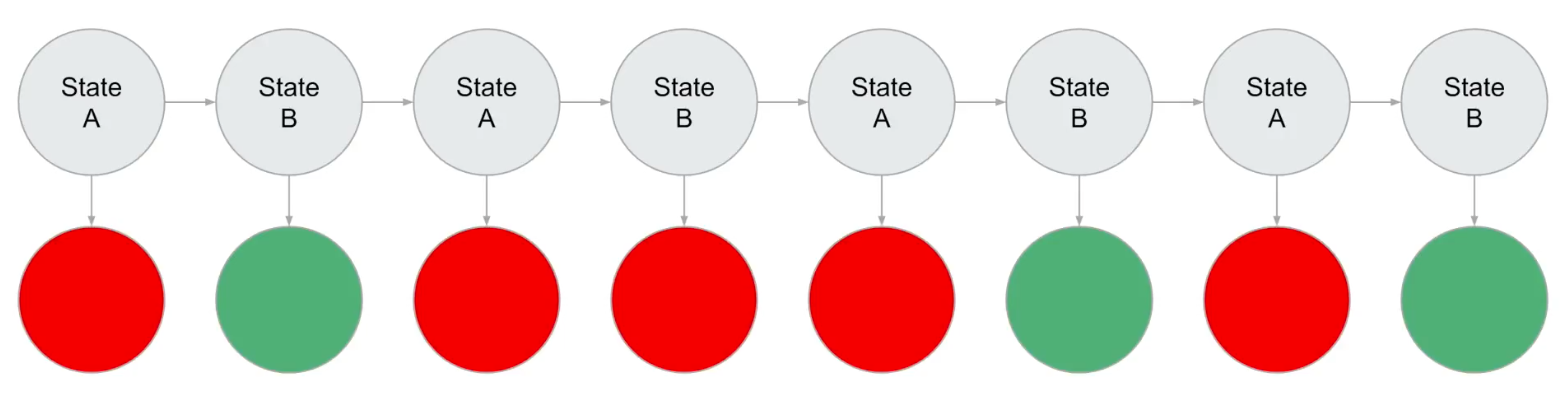
\includegraphics[scale=0.3]{hmm_example.png}
\caption{Visualization of a Hidden Markov Model. Upper circles represent hidden 
	states ($X_n$). Lower (colored) circles represent emitted observable states ($Y_n$)
	Adopted from \citep{hmm_figure}
	}
\label{fig:hmm}
\end{figure}

HMM is used to compute the likelyhood state sequences (often denoted
as \textit{hidden states}) of $X_n$ based on the 
observed sequence $Y_n$, conditional transition probability (often denoted
\textit{emission probability}) $P(Y_n \in A | X_n = x_n)$.
The Baum-Welch algorithm is used to fit the paramteres of the HMM based on the
observed data \citep{baggenstoss2001modified}. The Viterbi algorithm (described
in more detail in~\ref{sec:viterbi}) can be used to efficiently 
find the most likely sequence of hidden states based on 
the hidden state transition probabilities ($P(X_n | X_{n - 1})$,
emission probabilities ($P(Y_n | X_n)$), and initial state information $(P(X_1)$. 

HMM have been employed to model numerous tasks, such as 
speech recognition \citep{schuller2003hidden},
handwriting recognition, functional MRI brain mapping,  network anomaly
detection \citep{yu2010hidden} and many more.

\subsection{Viterbi algorithm}
\label{sec:viterbi}

The Viterbi algorithm is a recursive optimal solution to the problem of
estimating the state sequence of a discrete finite-state Markov process
\citep{howard1960dynamic} observed in memoryless noise
\citep{forney1973viterbi}. A Markov process is a stochastic process
whose future state values (time is discrete) are determined by
recent ones. Such a process generates a sequence of $T$ states 
$\textbf{x} = (x_0, \dots, x_T)$, where 
$x_t \in \{1, 2, \dots, K\}$, $\forall t \in {1, \dots, T}$
under the condition that :
$$
P(x_{t + 1} | x_0, x_1,\dots,x_t) = P(x_{t + 1} | x_t).
$$
Using the Viterbi algorithm it is then possible 
to find the most likley sequence of states -- 
the \textbf{Viterbi path}.

More formally, if we observe a sequence of
observations $\textbf{y} = (y_1, \dots, y_T)$ with output states
$y_i \in O = \{o_1, \dots, o_N\}$ with an initial state probability
probility array $\bm{\pi} = \{\pi_1,\dots, \pi_K\}$
behaving under a transition matrix $A$ of size $K \times K$
with element $A_ij$ storing the transition probability of
$s_i$ to $s_j$, 
and emission matrix $B$ of size $K \times N$ with 
element $B_ij$ storing probability of observing $o_j$ from $s_i$,
where $T$ is the number of steps, 
$K$ the number of possible states, and $N$ is the number of 
possible observations. We wish to find
$\textbf{x} = (x_1, \dots, x_T)$
as a sequence of states $x_i \in S = \{s_1, \dots, s_K\}$ 
most likely to generate the observed outputs under the 
conditions specified. 

A forward pass is made, which populates two
tables $T_1$ and $T_2$, both of size
$K \times T$. An element $T_1[i, j]$ stores 
probablities of the most likely path so far with 
$x_j = s_i$ that generates $\textbf{y} = (y_1, \dots, y_j)$.
$T_2[i, j]$ stores elements $x_{j - 1}$ of the most
likely path $\bm{\hat{x}} = (\hat{x}_1, \dots, \hat{x}_j = s_j)$:
\begin{align*}
T_1[i, j] = \max_k (T_1[k, j - 1] \cdot A_{ki} \cdot B_{iy_j}) \\
T_2[i, j] = \argmax_k (T_1[k, j - 1] \cdot A_{ki})
\end{align*}
calculated for each $k \in \{1, 2, \dots, K\}$, subsequence
of length $\forall j, 2 \leq j \leq T$

\subsection{Conditional Random Fields}
\label{sec:crf}

Conditional random fields (CRF) is a framework for building probablistic 
models to segment and label sequence data \citep{wallach2004conditional}
When trying to predict a vector $\mathbf{Y} = \{y_0, \dots, y_t\}$
of random variables given an observed feature vector 
$\mathbf{X} = \{x_0, \dots, x_t\}$. 
the typical supervised classification approach would be 
to learn independent classifiers to map $\forall i,  x \to y_i$
\citep{sutton2012introduction}.
However, this approach doesn't take into account possible dependencies
that may exist between labels, example being that neighboring 
regions in an image tend to have similar labels. 
Thus, predicting output variables can be represented as a graphical model.
Graphical models can be directed and undirected, but 
in the scope of this thesis, we limit ourselves to 
directed linear conditional random fields
and all subsequent definitions apply only to those. 
For an overview of other CRF, I recommend an
introductory, but comprehensive tutorial 
on CRFs \citep{sutton2012introduction} and the original paper on CRF by Lafferty et. al
\citep{lafferty2001conditional}. 

Formally, let $G = (V, E)$ be a graph such that $\mathbf{Y} = (\mathbf{Y}_v)_{v
\in V}$, so that $\mathbf{Y}$ is indexed by the vertices of $G$. Then
$(\mathbf{X}, \mathbf{Y}$) is a \textit{conditional random field} in case, when
conditioned on $\mathbf{X}$, the random variables $\mathbf{Y}_v$ obey the
Markov property with respect to the graph: $p(\mathbf{Y}_v | \mathbf{X},
\mathbf{Y}_w, w \neq v) = p(\mathbf{Y}_v | \mathbf{X}, \mathbf{Y}_w, w \sim v)$
, where $w \sim v$ means that $w$ and $v$ are neighbors in $G$
\citep{lafferty2001conditional}. 
For the linear chain case, $G$ is a simple chain
defined by: $G = (V = \{1, \dots, m\}, E = \{(i, i + 1)\})$, making 
$\mathbf{X} = (\mathbf{X_1}, \mathbf{X_2}, \dots, \mathbf{X_t})$
and $\mathbf{Y} = (\mathbf{Y_1}, \mathbf{Y_2}, \dots, \mathbf{Y_t})$.
%as depicted in figure~\ref{fig:chaincrf}. 
Now, the joint distribution of $X$ and $Y$ over $T$ time steps 
can be factorized as:
$$
p(x, y) = \prod_{t=1}^{T} p(y_t | y_{t - 1}) p(x_t | y_t)
$$
By setting $\theta_{ij} = \log p(y' = i | y = j)$ and
$\mu_{oi} = \log p(x = o | y = i)$ the joint distribution
can be rewritten as:
$$
p(x, y) = \frac{1}{Z} \prod_{t=1}^{T} exp \left\{ \sum_{i, j \in S} \theta_{ij} \mathbf{1}_{\{y_t=i\}} \mathbf{1}_{\{y_{t-1} = j\}}
+ \sum_{i \in S} \sum_{o \in O} \mu_{oi} \mathbf{1}_{\{y_t = i\}}\mathbf{1}_{\{x_t  = o\}} \right\}
$$
where $\theta = \{theta_{ij}, \mu_{oi}\}$ are parameters of the distribution and $Z$ is the
normalization constant. This can be shortened by 
introducing a \textit{feature function}
defined as $f_k (y_t, y_{t - 1}, x_t)$:
$$
p(x, y) = \frac{1}{Z} \prod_{t=1}^{T} exp \left\{ \sum_{k=1}^{K} \theta_k f_k(y_t, y_{t - 1}, x_t) \right\}
$$
Now, we can derive conditional distribution $p(y | x)$:
\begin{equation}\label{eq:cond_crf}
p(y | x) = \frac{p(y, x)}{\sum_{y'} p(y', x)}  = 
\frac{\prod_{t=1}^{T} exp \left\{ \sum_{k=1}^{K} \theta_k f_k(y_t, y_{t - 1}, x_t) \right\}}
{\sum_{y'} \prod_{t=1}^{T} exp \left\{ \sum_{k=1}^{K} \theta_k f_k(y'_t, y'_{t - 1}, x_t) \right\}}
\end{equation}
which is the definition of the \textit{linear-chain conditional random field}.
This definition can be extended such that the feature function can depend on 
multiple inputs, as the vector $x_t$ (representing all observations of $x$
until time step $t$) can be a parameter of the feature function $f_k$. 

Deriving inference in CRFs (finding 
$y^* = \argmax_y p(y | x)$) 
in the general case is intractable since 
it requires computing all possible $p(y_t, y_{t - 1} | x)$ 
and the normalizing constant $Z$, which grows exponentially with the 
sequence length. 
However, in the case of the linear-chain CRF it is possible to 
use dynamic-programming algorithms, such as the
forward-backward algorithm \citep{devijver1985baum} 
for computing the marginal distributions and 
the Viterbi algorithm
(section~\ref{sec:viterbi}) for computing
the most probable assignment. 
To estimate parameters $\theta$ of a conditional 
random field \textit{maximum likelyhood} is used.
A training dataset of $N$ samples $\{\mathbf{x}^{(i)}, \mathbf{y}^{(i)}\}^{N}_{i=1}$
where each $\mathbf{x}^{(i)} = \{x_{1}^{(i)}, \dots, x_{T}^{(i)}\}$
is a sequence of inputs
and $\mathbf{y}^{(i)} = \{y_{1}^{(i)}, \dots, y_{T}^{(i)}\}$ is 
a sequence of labels. To esimate parameters, we
minimize log likelyhood expressed as a function of parameters $\theta$:

$$
\theta^{*} = \argmin_{\theta} \sum_{i=1}^{N} \log p(\mathbf{y}^{(i)} | \mathbf{x}^{(i)} ; \theta)
$$
Expanding the conditional likelyhood using the definition of conditional random field
(equation~\ref{eq:cond_crf}) and adding an $L_2$ regularization factor $1/2 \sigma^2$ 
to penalize large weights:
$$
\sum_{i=1}^{N} \sum_{t=1}^{T} \sum_{k=1}^{K} \theta_k f_k (y_{t}^{(i)}, y_{t - 1}^{(i)} x_{t}^{(i)}) 
- \sum_{i=1}^N \log Z(x^{(i)}) - \sum_{k=1}^{K} \frac{\theta_{k}^{2}}{2 \sigma^2}
$$
Deriving to find the optimal set of $\theta$, we end up with:
$$
\frac{\partial }{\partial \theta_k} = \sum_{i=1}^{N} \sum_{t=1}^{T} f_k (y_{t}^{(i)}, y_{t - 1}^{(i)} x_{t}^{(i)}) 
- \sum_{i=1}^{N} \sum_{t=1}^{T} \sum_{y, y'} f_k (y, y', x_{t}^{(i)}) p(y, y'|x^{(i)}) - \frac{\theta_k}{\sigma^2}
$$
The result is a concave function (which is useful since we're looking for the 
maximum) since it is of the form $\log \sum_i \exp x_i$, thus can be optimized by
any hill climbing technique, with the 
Broyden-Fletcher-Goldfarb-Shanno algorithm \citep{liu1989limited} being a popular 
choice. 

CRFs, particularly linear-chain CRFs
have been widely applied in natural language processing in tasks such as
named entity recognition \citep{liu2011recognizing}, shallow parsing \citep{sha2003shallow}, 
extracting syntax from text \citep{taskar2004max}, 
semantic role labeling \citep{cohn2005semantic}, citation extraction \citep{wellner2004integrated}, 
sentiment analysis \citep{patra2014ju_cse} and many more. 

%TODO Applications of CRF
% Extracting syntax from natural-language text 

% \begin{figure}
% 	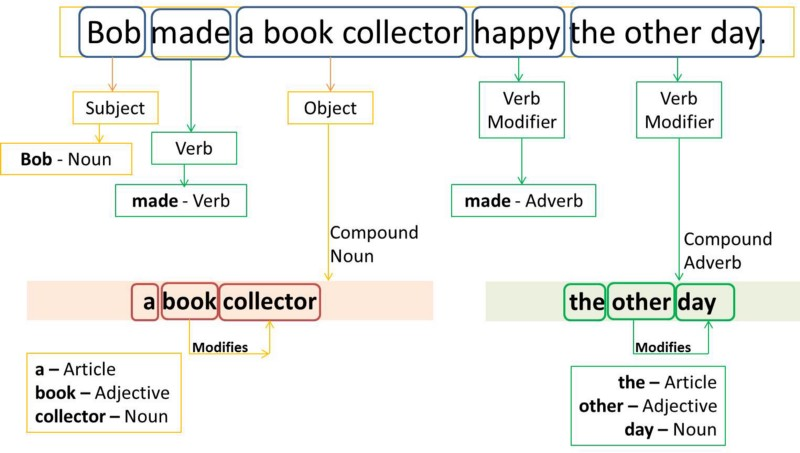
\includegraphics[scale=0.55]{pos_example.jpeg}
% \end{figure}
\begin{figure}
	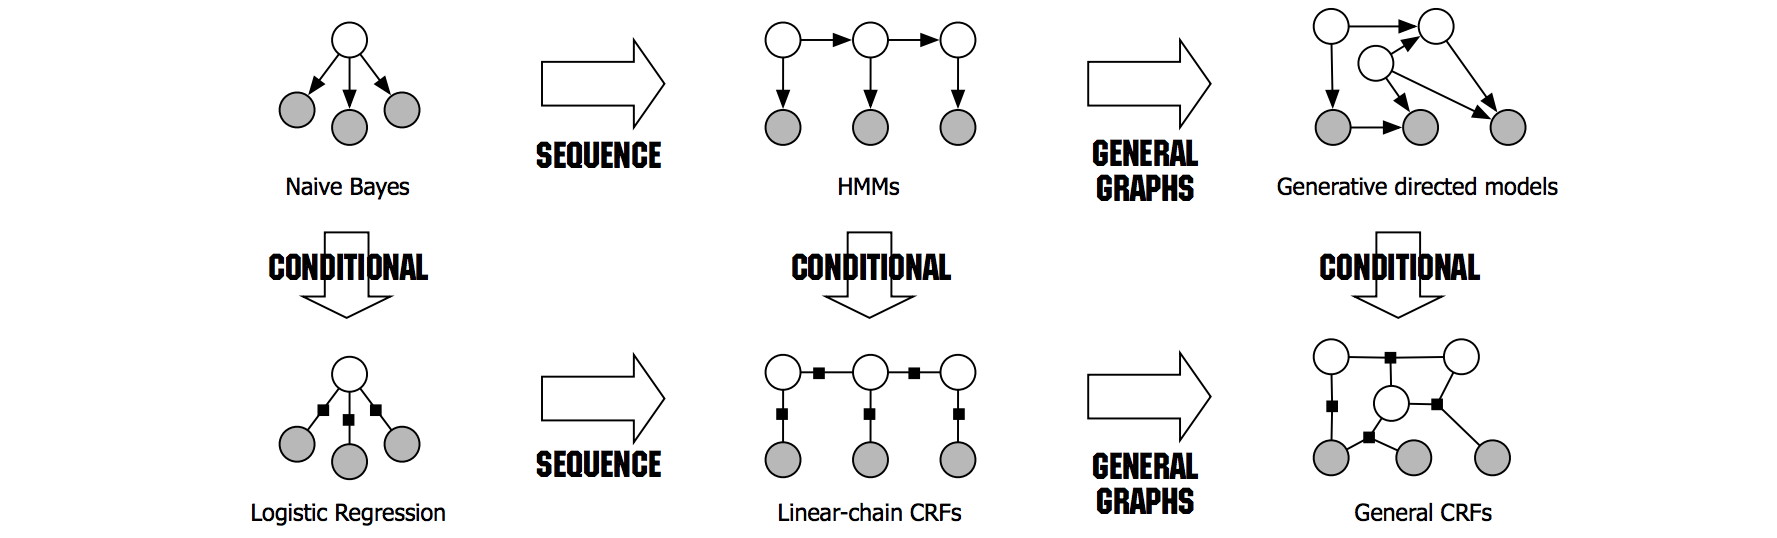
\includegraphics[width=\textwidth]{different_markovs.png}
	\caption{Visualization of differences between generative and discriminative approaches
	as well as sequential and non sequential approaches.
	Adopted from \citep{sutton2012introduction}}
	\label{fig:different_graphicals}
\end{figure}

% \begin{figure}
% 	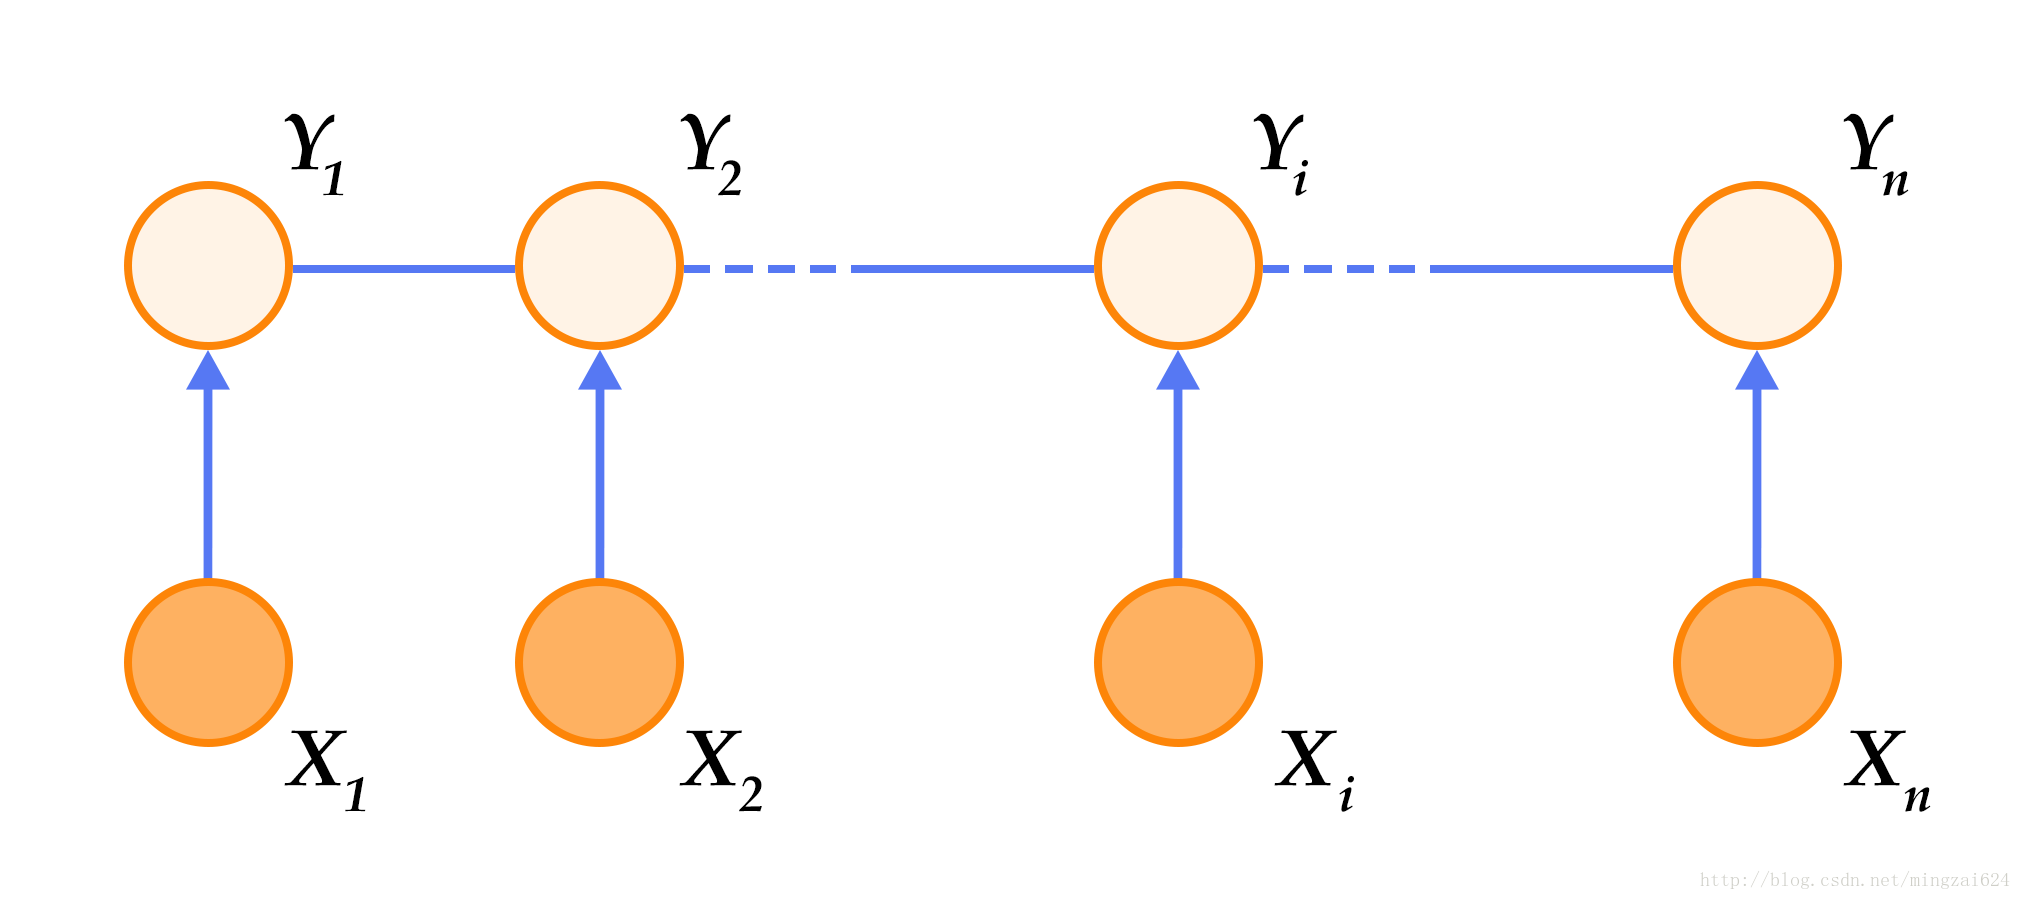
\includegraphics[scale=0.23]{chain_crf.png}
% 	\caption{Linear chain conditional random field \citep{chaincrffigure}}
% 	\label{fig:chaincrf}
% \end{figure}


\subsection{LSTM-CRF Model for Sequence Tagging}

\begin{figure}
	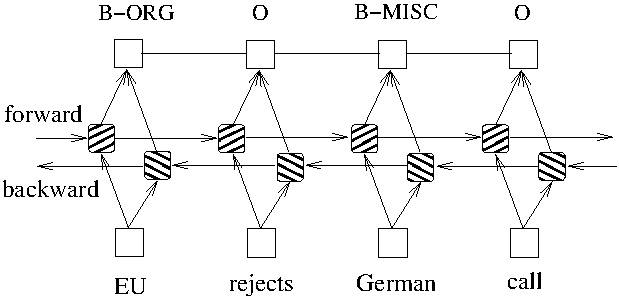
\includegraphics[width=0.8\textwidth]{biLstmCRF.pdf}
	\caption{A BiLSTM CRF model. Adopted from 
	\citep{huang2015bidirectional}
	}
	\label{fig:bilstm_crf}
\end{figure}


LSTM networks do a very good job of encoding sentences
(see section~\ref{sec:lstm}) to perform classification using only 
word embeddings as features (more on embeddings in section),
%TODO add reference
but do not take neighboring label information when performing sequence
classification which is important to solve sequence tagging
problems (such as named entity recognition \citep{nadeau2007survey}).
CRFs (see section~\ref{sec:crf}) allow for modeling label level 
dependencies and can work with arbitrary features, which have usually been
handcrafted.
Therefore, using an LSTM layer to encode words as features can be an input to a
CRF model which then uses standard 
parameter estimation to estimate its parameters. 
The combination of a bi-directional LSTM and a CRF is shown in figure~\ref{fig:bilstm_crf}.

CRF can use an arbitrary feature function $f_k$
to define its conditional probability (~\ref{eq:cond_crf}).
This feature function can 
be understood as the score of how well the sequence 
of states $y$ fit the given input $x$ and parameters $\theta$:
This score can be calculated as
:
$$
s_{LSTM-CRF}(x, y) = \sum_{t=0}^{T} \left( A_{t, t-1} + LSTM(x_t) \right)
$$
where $A$ is the transition matrix between states of $y$ with element
$A_{t, t-1}$ is the transition from state $y_{t-1}$ to state $y_{t}$, and $LSTM$
encodes input sentence using an LSTM network.
Dynamic programming methods (such as Viterbi~\ref{sec:viterbi}) can be used 
to efficiently compute optimal tag sequences
for inference. More details can be found in \citep{huang2015bidirectional}.

\subsection{Chain classification}
\label{sec:chain_classification}

Multilabel classification is a classification problem where 
a single instance may be assigned more than one class, making it 
a generalization of multiclass classification.
Formally, multiclass classification is the problem of finding 
a model that maps $x$ to binary vectors $y$, $y \in L = \{1, 2, \dots, N\}$. Typically, 
multilabel classification is usually framed as either:
\begin{enumerate}
	\item transformation into binary classification problems -- \textit{binary relevance} (BR) \citep{luaces2012binary} or
	\item transformation into multiclass problems \textit{label powerset} (LR).
\end{enumerate}
The binary relevance method transforms multilabel classification
into multiple binary problems; one problem for each label, such that each
binary model is trained to predict the relevance of one of the labels
\citep{read2011classifier}. This method trains $|L|$ binary classifiers
$C_1, \dots, C_{|L|}$ where each classifier $C_j$ predicts the $0/1$ association
for each correponding label $l_j \in L$ \citep{read2011classifier}.
Transforming from multi-label to binary with the BR method,
label correlations that might exist in training data are ignored, therefore
predicted labels might contain label combinations that might never occur in practice. 

\begin{figure}
\begin{algorithmic}[1]
\For{$j \in 1 \dots |L|$}
  \State $D' \gets \{\}$
	\For{$(x, S) \in D$}
	  \State $D' \gets D' \cup (x, l_1, \dots, l_{j - 1}, l_j)$
	  \State $C_j: D' \gets l_j \in \{0, 1\}$
	\EndFor
\EndFor
\end{algorithmic}
\caption{Classifier chain training phase for dataset 
	$D = \{(x_1, S_1), \dots, (x_n, S_n)\}$
	and label set $L$.
	Adopted from~\citep{read2011classifier}
	}

\label{alg:train_chain_classifier}
\end{figure}

\begin{figure}
\begin{algorithmic}[1]
\State $Y \gets \{\}$
\For{$j \in 1 \dots |L|$}
  \State $Y \gets Y \cup (l_j \gets C_j: (x, l_1, \dots, l_{j - 1})$
\EndFor
\Return $(x, Y)$
\end{algorithmic}
\caption{Classifier chain prediction phase for instance $x$ 
	and label set $L$.
	Adopted from~\citep{read2011classifier}
	}
\label{alg:test_chain_classifier}
\end{figure}

The label powerset method combines entire label sets into atomic labels 
to form a single-label problem for which the set of possible labels 
represents all distinct label subsets in the original multi-label 
representation. Each example $(x_i, S)$ is transformed into 
$(x_i, l)$, where $S$ represents the label combination set and
$l$ represents an atomic label representing the same combination set $S$
\citep{read2011classifier}. LR takes into 
consideration label correlations, but the number of combinations
is exponentially dependent on the number of labels $2^{|L|}$. 

The classifier chain method ($CC$) involves $|L|$ binary classifiers as in BM. 
Classifiers are chained such that each classifier deals with 
a single binary relevance problem $l_j \in L$ using an extended feature space of 
previous classifiers 
forming a chain of classifiers \citep{read2011classifier}.
The training phase is outlined in figure~\ref{alg:train_chain_classifier}. 
Each classifier $C_j$ in the chain is responsible for predicting 
the binary association of label $l_j$ using all prior 
binary relevance predictions in the chain $l_1, \dots, l_{j - 1}$.
The classification starts with $C_1$ determining 
$prediction(l_1 | x)$ propagating along the chain
to predict $prediction(l_j | x_i, l_1, \dots, l_{j-1})$, outlined 
in figure~\ref{alg:test_chain_classifier}
\citep{read2011classifier}.
The idea of the chaining method is to overcome the label independence problem
inherent to BM, retaining lower complexity advantages. 
For a more detailed complexity analysis see \citep{read2011classifier}. 
However, the ordering labels to train can have a significant effect on 
the classification accuracy. 

To overcome the ordering problems of classifier chains, one
can perform ensembling. 
Ensembling methods are learning algorithms 
that construct a set of classifiers and then classify new data 
points by taking a (weighted) vote of their predictions \citep{dietterich2000ensemble}.
Ensembling has proven to be succesful for multi-label 
problems, especially since it is usually easy to paralelize. 
\citep{tsoumakas2007random}. Classifier chains can also be
ensembled to try and overcome the ordering bias. An Ensemble 
Classifier Chain ($ECC$) trains $m$ chain classifiers training
each classifier with a random chain ordering (of $L$) and a random
subset of the dataset. Predictions of each  model $C_k, k \in \{1, \dots, m\}$ 
are then summed so that each label receives a number of votes
\citep{dimitriadou2001voting}.

\section{Unsupervised Machine Learning}
\label{sec:unsupervised_machine_learning}

As opposed to supervised machine learning (described in
section~\ref{sec:machine_learning}), unsupervised machine learning
has no access to labeled data. The goal of unsupervised machine learning,
often denoted as \textit{clustering} is to separate 
a finite unlabeled dataset into a finite and discrete set of 
\textit{natural} hidden data structures \citep{xu2005survey}.
Evaluating resulting clusters can be subjective, as there is a mere 
requirement that patterns in the same cluster should be similar to each
other, more than patterns in other clusters. More formally, 
given a set of input patterns $X = \{x_1, \dots, x_N\}$, where
$x_j = (x_{j1}, \dots, x_{jd})$ partitioning (clustering) can 
be performed in two ways \citep{xu2005survey}:
\begin{description}
\item[Hard clustering] seeks to partition $X$ into $K$ partitions $C=\{C_1, \dots, C_K\}, K \leq N$
	such that 
	\begin{enumerate}
	\item $C_i \neq \emptyset, i = 1, \dots, K$, 
	\item $\cup_{i=1}^{K} C_i = X$, and
	\item $C_i \cap C_j = \emptyset , i, j = 1, \dots K$ and $i \neq j$.
	\end{enumerate}
\item[Hierarchical clustering] constructs a tree-like partition of $X$ as 
	$H = \{H_1, \dots, H_Q\}, Q \leq N$ such that
	$C_i \in H_m, C_j \in H_n$ and $m > n$
	imply $C_i \in C_j$ or $C_i \cap C_j = \emptyset, \forall i, j, j \neq
		i, m = 1 \dots Q, l = 1 \dots Q$
\end{description}

\begin{figure}
	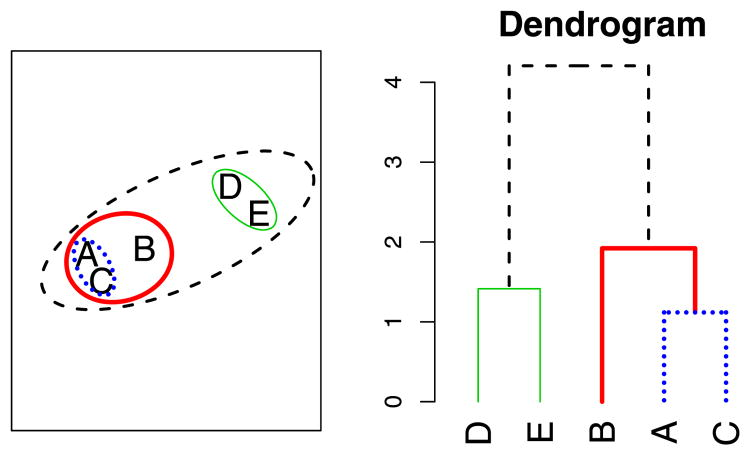
\includegraphics{clustering_linkage.jpg}
	\caption{
		Agglomerative hierarchical clustering produces a sequence of
		clusterings that can be represented as a dendrogram. Each
		interior node of the dendrogram corresponds to a merging of two
		clusters. Adopted from \citep{bien2011hierarchical}
	}

	\label{fig:clustering}
\end{figure}

\subsection{Hierarchical clustering}
\label{sec:hierarhical_clustering}

Hierarchical clustering is further subdivided into:
\begin{description}
	\item[Agglomerative]: a ``bottom-up'' approach where each observation
		starts in a single cluster and pairs of clusters are merged up the hierarchy and
	\item[Divisive]: a ``top-down'' approach where all observations start in one cluster on which
		splits are recursively performed down the hierarchy.
\end{description}
An example of agglomerative clustering is shown in figure~\ref{fig:clustering}. 
In order to determine which clusters should be combined (in the agglomerative case) or 
split (in the divisive case) there have to be defined measures of distance and a \textit{linkage 
criterion} which specifies the dissimilarity of clusters based on pairwise observation 
distances. Some common distance measures between two observations $a$ and $b$ are:
\begin{description}
	\item[Euclidan]: $||a - b||_2 = \sqrt{\sum_i (a_i - b_i)^2}$, 
	\item[Manhattan]: $||a - b||_1 = \sum_i |a_i - b_i|$, and
	\item[Maximum]: $||a - b||_{\infty} = \max_i |a_i - b_i|$.
\end{description}
and some common linkage criterion (according to \citep{szekely2005hierarchical}
between two clusters of observations $A$ and $B$ 
using distance metric $d$ are:
\begin{description}
	\item[Complete linkage]: $\max \{d(a, b): a \in A, b \in B\}$,
	\item[Minimum linkage]: $min \{d(a, b): a \in A, b \in B\}$,
	\item[Unweighted linkage]: $\frac{1}{|A| \cdot |B|} \sum_{a \in A} \sum_{b \in B} d(a, b)$,
	\item[Weighted average linkage]: $d(i \cup j, k) = \frac{d(i, k) + d(j, k)}{2}$, and
	\item[Ward's linkage] that minimizes the total within-cluster variance. It is calculated as
		$$
		\sum_{i \in A \cup B} ||x_i - m_{A \cup B}||^2 - \sum_{i \in A}||x_i - m_A||^2 
		- \sum_{i \in B} ||x_i - m_B||^2
		$$ 
		where $m_j$ is the center of cluster $j$  and $x_i$ is a datapoint
		in cluster $i$ \citep{ward1963hierarchical}.
\end{description}

% \citep{kaufman2009finding}
% \citep{reynolds2006clustering}

\subsection{Evaluation Methods}
\label{sec:clus_evaluation}

One standard way to evaluate the result of clustering is by
calculating the silhouette score \citep{reynolds2006clustering}. 
Let $C_M = \{C_1, \dots, C_k\}$ describe a clustering result, an 
exhaustive partitioning of dataset $D$. Then define the mean distance
between a single instance $i$ in cluster $C_i$ and all other points in the same cluster as
$$
a(i) = \frac{1}{|D_i| - 1} \sum_{j \in C_i, i \neq j} d(i, j)
$$
where $d(i, j)$ is the distance between data points $i$ and $j$ in
the cluster $C_i$. Then, define mean dissimilarity of an instance $i$ to
clusters it does not belong to $C \neq C_i$ as
$$
b(i) = \min_{k \neq i} \frac{1}{|C_k|} \sum_{j \in C_k} d(i, j)
$$.
Now, silhouette value of a single instance $i$ is defined as:
\begin{align}\label{eq:silhouette}
	s(i) &= \frac{b(i) - a(i)}{\max\{a(i), b(i)\}} \textrm{, if } |C_i| > 1 \\
	s(i) &= 0 \textrm{, if } |C_i| = 1
\end{align}
with $-1 \leq s(i) \leq 1$. Silhouette score close to $1$ means that a data point $i$
is very well matched with respect to the neighboring cluster, having large $a(i)$, whereas
having a large $b(i)$ makes silhouette score close to $-1$ implying that a data point is badly matched 
and it might be more appropriate to have it in the neighboring cluster. 
Silhouette score reflects how tightly grouped all data points in the cluster are
\citep{kaufman2009finding}.

\begin{table}
	\centering
	\begin{tabular}{c c c c c c c}
		\toprule
		Partition & & \multicolumn{4}{c}{$C$} & \\ \cline{3-6}
		& Group & $C_1$ & $C_2$ & \dots & $C_r$ & Total \\
		\midrule
		\multirow{4}{*}{$D$} & $D_1$ & $t_{11}$ & $t_{12}$ & \dots & $t_{1r}$ & $t_{1.}$ \\
		                     & $D_2$ & $t_{21}$ & $t_{22}$ & \dots & $t_{2r}$ & $t_{2.}$ \\
				     & $\vdots$ & $\vdots$ & $\vdots$ & $\ddots$ & $\vdots$ & $\vdots$ \\
		                     & $D_s$ & $t_{s1}$ & $t_{s2}$ & \dots & $t_{sr}$ & $t_{s.}$ \\
				     \midrule
		Total & &                      $t_{.1}$ & $t_{.2}$ & $\dots$&$t_{.r}$ & $t_{..} = N$ \\
				     \bottomrule
	\end{tabular}
	\caption{Adjusted rand index contigency table, adapted from \citep{santos2009use}}
	\label{tab:adjusted_rand}
\end{table}

\textit{Rand Index} is a measure of similarity between two clusters. \citep{santos2009use}
Given a dataset $X = \{x_1, \dots, x_N\}$ partitioned into two clustering results
$C = \{C_1, \dots, C_r\}$ and $D = \{D_1, \dots, D_s\}$ consisting of $r$ and $s$ clusters
respectively, define:
\begin{itemize}
\item $a$ as the number of pairs in $X$ that are in the same cluster in $C$ and $D$,
\item $b$ as the number of pairs in $X$ that are in different clusters in $C$ and $D$,
\item $c$ as the number of pairs in $X$ that are in the same clusters in $C$ and in different clusters of $D$, and
\item $d$ as the number of pairs in $X$ that are in different clusters in $C$ and in the same clusters in $D$. 
\end{itemize}
Rand index is then defined as:
\begin{equation}\label{eq:rand_index}
	R = \frac{a + b}{a + b + c + } = \frac{a + b}{\binom{n}{2}}
\end{equation}
where $a + b$ and $c + d$ reflects similarity and dissimilarity of two clusterings respectively.  
$\binom{n}{2}$ reflect the chance that two clusterings will randomly agree on a chosen pair. 
The Rand Index ($0 \leq R \leq 1$) value reflect how well two clusterings agree, with 
$0$ indicating complete disagremeent and $1$ signaling exactly same clusterings. 
\textit{Adjusted Rand Index} (ARI) is derived from Rand Index, but it is corrected for chance
\citep{steinley2004properties}. To calculate ARI, a contigency table is usually built which, 
given a dataset $X = \{x_1, \dots, x_N\}$ partitioned into two clustering
results $C = \{C_1, \dots, C_r\}$ and $D = \{D_1, \dots, D_s\}$ consisting of
$r$ and $s$ clusters, calculates the number of objects $n_{ij}$ common for every
$C_i$ and $D_j$, $t_{ij} = |C_i \cap D_j|$. Then row and column sums are calculated 
as shown in table~\ref{tab:adjusted_rand} using which ARI is calculated as:
\begin{equation}\label{eq:adjusted_rand_index}
	ARI = \frac{\sum_{ij} \binom{t_{ij}}{2}- \left[ \sum_i \binom{t_{i.}}{2} \sum_j \binom{t_{.j}}{2} \right] / \binom{N}{2}}
	{\frac{1}{2} \left[ \sum_i \binom{t_{i.}}{2} + \sum_j \binom{t_{.j}}{2} \right] - 
	\left[ \sum_i \binom{t_{i.}}{2} \sum_j \binom{t_{.j}}{2} \right] / \binom{N}{2}
	}
\end{equation}

\textit{V-measure} is an external entropy-based cluster evaluation measure which measures
how succesfully the criteria of homogeneity and completeness have been satisfied. 
\citep{rosenberg2007v}
It is computed as a harmonic mean of distinct homogeneity and completeness scores. 
\textit{Homogeneity} examines how close a given clustering $C = \{c_1, \dots, c_n\}$ of 
$N$ data points is to an ideal $K = \{k_1, \dots, k_m\}$ (members of a single
class should be in a single cluster) clustering by calculating the 
conditional entropy of the class distribution given the proposed clustering 
$H(C | K)$:
$$
h = 1 - \frac{H(C | K)}{H(C)}
$$
where 
\begin{align*} 
	H(C | K) &= - \sum_{k=1}^{|K|}\sum_{c=1}^{|C|} \frac{t_{ck}}{N}\log \frac{t_{ck}}{\sum_{c=1}^{|C|} t_{ck}} \\
	H(C) &= - \sum_{c=1}^{|C|} \frac{\sum_{k=1}^{K} t_{ck}}{n} \log \frac{\sum_{k=1}^{|K|} t_{ck}}{n}
\end{align*}
where $t_{ck}$ is a value in the contigency table between two clusterings as shown in table~
\ref{tab:adjusted_rand}.
To satisfy the \textit{completeness} criteria, a clustering must assign all 
members of a single class to a single class, making it symetrical to 
homogeneity, calculated through conditional entropy of the proposed clustering
given the class of datapoints $H(K | C)$:
$$
c = 1 - \frac{H(K | C)}{H(K)}
$$
where
\begin{align*}
H(K | C) &= - \sum_{c=1}^{|C|}\sum_{k=1}^{|K|} \frac{t_{ck}}{N} \log \frac{t_{ck}}{\sum_{k=1}^{|K|} t_{ck}} \\
H(K) &= - \sum_{k=1}^{|K|} \frac{\sum_{c=1}^{C} t_{ck}}{n} \log \frac{\sum_{c=1}^{|C|} t_{ck}}{n}
\end{align*}
where $t_{ck}$ is a value in the contigency table between two clusterings as shown in table~
\ref{tab:adjusted_rand}.
Now, through homogeneity $h$ and completeness $c$, we define V-measure as:
\begin{equation}\label{eq:v-measure}
	V = (1 + \beta) \cdot \frac{h \cdot c}{\beta \cdot h + c}
\end{equation}

% Adjusted Rand Index (ARI) (Hubertand Arabie, 1985) and the
% information-theoretic V-measure (Rosenberg and Hirschberg, 2007

\section{Natural Language Processing}
\label{sec:natural_language_processing}

Natural Language Processing (NLP) is a subfield of lingustics, computer
science, and artificial intelligence concerned with how to program computers to
process and analyze natural language data, text.  Natural Language Processing
techniques rely heavily on machine learning and statistical models which learn
from large amounts of textual data.  There are many subareas of natural
language processing, such as syntax, semantics, and discourse analysis.
Each of the subareas attempts to solve a set of problems, sentiment analysis, named
entity recognition, distributional semantics, recognizing textual entailment being
some of the problems of semantics. Good, yet comprehensive introductions to NLP are available 
in many books \citep{manning1999foundations} and review papers \citep{collobert2011natural}. 
Argumentation
mining is considered to closely related to natural language processing
\citep{lippi2015argument}, as it uses commonly used natural language processing
techniques to work on problems from social sciences to analyze arguments.
In the rest of this section, we give a introduction on various word representations
in subsections~\ref{sec:bow},~\ref{sec:tf-idf}, and~\ref{sec:embedding}, 
then we go into more detail on two 
semantics-related NLP problems: textual entailment in subsection~\ref{sec:textual_entailment}
and semantic textual similarity in subsection~\ref{sec:sts}.

\subsection{Bag-of-words}
\label{sec:bow}
In information retrieval it is often 
vital to efficiently 
store (index) and search collections of documents. 
To do so, documents are represented as features. 
One of the simplest document representations is applying the 
\textbf{bag-of-words} (BoW) model to text. BoW represents text as a multiset of
words along with their respective frequencies of occurence. However, it disregards
grammar and word order
\citep{harris1954distributional}, hence the term ``bag''. 
We show an example of calculating BoW
using an excerpt from \citep{dickens1949tale}:
\begin{quote}
``\emph{It was the best of times, \\
it was the worst of times, \\
it was the age of wisdom, \\
it was the age of foolishness,
}''
\end{quote}
We treat each line of the example as a document $D_i$ in the set of documents
$D$. The vocabulary $V$ is 
defined as all the unique words (ignoring case and punctuation)
across the document collection:
$$
V = \{t_{ij} | w_{ij} \in D_i \cap i \in \{1 \dots |D|\} \}
$$
For this example, the vocabulary amounts to
$V = \{$\emph{``it'', ``was'', ``the'' ``best'', ``of'', ``times'', ``worst'', ``age'',
``wisdom'', ``foolishness''}$\}$.
Now, for each word of the vocabulary, we calculate the frequency in the document. 
A BoW representation of document $D_4$ 
``\emph{it was the age of foolishness}''
would then be: $x_4 = [1, 1, 1, 0, 1, 0, 0, 1, 0, 1]$

The \textbf{n-gram} document recepresentation is a generalization of the BoW
approach. The ngram model
can use multiple words ($n$) to represent a document preserving some spatial information.
The bigram model ($n = 2$) uses pairs of words to represent a document
The document $D_4$ using a bigram model would then consist of:
\emph{``it was'', ``was the'', ``the age'', ``age of'', ``of foolishness''}.
BoW is a specialization of the ngram model
that sets $n=1$. 

The BoW model has been succesfully applied to many areas, such as language
modeling \citep{tirilly2008language}, sentiment analysis
\citep{wang2014microblog}, and spam classification \citep{kolari2006detecting}.
BoW models are
usually used with an assumption that similar documents have only similar
content. After transforming text into the BoW form, extra features can be
calculated, such as tf-idf or embedding features. 

\subsection{Tf-idf}
\label{sec:tf-idf}
%\label{sec:word_representations}
Some other commonly used features  to represent text are \textbf{term frequency
tf} and \textbf{inverse document frequency idf}. Term frequency of a word is
the number of occurences of that word in a given document:

$$
\mathit{tf}(t, d) = \frac{f(t, d)}{|d|}
$$
where $f(t, D_i)$ is the frequency of term (word) $t$ in document $D_i$ and $|D_i|$ is the number
of total terms in document $D_i$.
Inverse document frequency is a measure of how much information a word provides (common or rare
across a collection of documents) as is calculated as:

\begin{equation}
	\label{eq:idf}
\mathit{idf}(t, D) = \log \frac{N}{1 + |D_i \in D: t \in D_i|}
\end{equation}
where $N$ is the number of documents in the corpus $|D|$ and $|D_i \in D: t \in D_i|$ is the 
number of documents in which term $t$ appears in. 
These two features are often used together to represent a collection of documents 
$D_i \in D$ each containing a list of terms $t$:
$$
\mathit{tfidf} (t, D_i, D) = \mathit{tf}(t, D_i) \cdot \mathit{idf}(t, D)
$$
The vector space model \citep{meadow1992text} treats text documents as vectors  
in an $N$-dimensional space, where $N$ is the size of the vocabulary (total number of 
possible words). Comparing two documents in the vector space model can then be taking the
cosine similarity of the vectors features.

\subsection{Word embeddings}
\label{sec:embedding}

Another word representation approach represents each word using a fixed-size
vector of real numbers. A set of such approaches is called \textit{word
embeddings}. These vector representations of words are generated through
different methods, most popular two being neural networks and word co-occurence
matrix dimensionality reduction.

\begin{figure}
	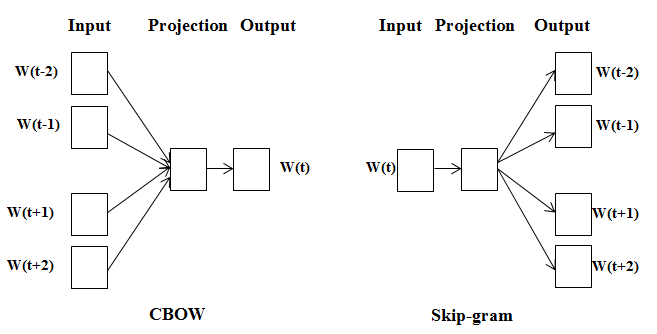
\includegraphics[scale=0.65]{skip_gram_cbow.png}
	\caption{CBOW (left) and skip-gram (right) simplified model architectures. Adopted from 
	\citep{suleiman2017deep}. }
	\label{fig:skip_gram_cbow}
\end{figure}

Word2vec is a neural network-based approach to generate distributed
representations of words \citep{mikolov2013distributed}.  It utilizes two
neural network models: a continuous \textit{bag-of-words} (CBOW) and continuous
\textit{skip-gram} approach.  The CBOW architecture is framed as a supervised
learning problem, where the model predicts the current word from a window of
surrounding context words. 
The ordering of the context words is not taken into
account (bag-of-words).  In the continuous skip-gram architecture, the model
uses the current word to predict the surrounding window of context words.
Architectures of both models are shown in figure~\ref{fig:skip_gram_cbow}. 
Models are then trained on large corpora, such as the Google Books corpus 
\citep{lin2012syntactic}. 
More details on training the models is available in the original word2vec papers
\citep{mikolov2013distributed, mikolov2013efficient}, as well as follow up papers
\citep{goldberg2014word2vec, rong2014word2vec}.
FastText is another word embedding procedure which is an extension on word2vec
\citep{bojanowski2017enriching}. In fastText each word is represented as a
n-gram of characters in order to capture the meaning of shorter words and allow
for embeddings to understand prefixes and suffixes. After splitting words into
subwords, similar procedures as the word2vec model are applied. 
The biggest advantage of using fastText is seen when dealing 
with rare words, which can be assigned a representation even if the word was
never seen during the model training period. 

\subsection{Textual Entailment}
\label{sec:textual_entailment}

\textit{Textual entailment} (TE) is defined as a directional relationship
between pairs of text expressions, denoted by $T$ --- the entailing ``Text'',
and $H$ --- the entailed ``Hypothesis''. We say that $T$ entails $H$ if,
typically, a human reading $T$ would infer that $H$ is most likely true 
\citep{dagan2005pascal}.  This definition assumes common human understanding of
language as well as common background knowledge. Examples of textual entailment
are in
table~\ref{tab:te_examples}.  
Recognizing textual entailment was established as
a popular natural language processing problem with the start of the
\textit{Recognising Textual Entailment} (RTE) challenge. The challenge involved
teams producing models to solve the TE problem on multiple datasets. A dataset
instance contained two sentences and a label whether entailment holds or not
($\mathit{True}$ or $\mathit{False}$).
Follow up challenges were organized \citep{bar2006second, giampiccolo2007third}.

\begin{table}
	\centering
	\begin{tabular}{p{8cm} | p{5cm} | c}
		Text & Hypothesis & TE \\
		\toprule
		\textit{
		Norway’s most famous painting, ``TheScream'' by Edvard Munch, was recov-ered
		Saturday, almost three months after it was stolen from an Oslo
		museum.} & 
		\textit{Edvard   Munch   painted ``The Scream''  }
		& $\mathit{True}$ \\
		\textit{Republic of Yemen is an Arab, Islamic and independent
		sovereign statewhose integrity is inviolable,  and  no part
		of which may be ceded.} & 
		\textit{The national language of Yemen is Arabic.}
		& $\mathit{True}$ \\
		\textit{Regan attended a ceremony in Washington to commemorate the
		landings in Normandy.} &
		\textit{Washington is located in Normandy. } & $\mathit{False}$ \\
		\bottomrule
	\end{tabular}
	\caption{Positive and negative examples of Textual Entailment (TE) 
	Adopted from \citep{dagan2005pascal}}
	\label{tab:te_examples}
\end{table}

Textual Entailment is closely related to the task of \textit{natural language inference} (NLI), 
where each pair of sentences can be assigned one of three possible labels:
\begin{enumerate*}
	\item entailment, 
	\item neutral, and
	\item contradiction. 
\end{enumerate*} 
making it more general than the TE challenge. 
The most used dataset of NLI is the Stanford Natural Language Inference dataset
\citep{bowman2015large} which contains 570K pairs of labelled sentence pairs. 
Examples of the dataset are available in table~\ref{tab:snli_examples}.

\begin{table}
	\centering
	\begin{tabular}{p{8cm} | p{5cm} | c}
		Text & Hypothesis & Relation \\
		\toprule
		\textit{
		A man inspects the uniform of a figure in some East Asian country.
		museum.} & 
		\textit{The man is sleeping}
		& $\mathit{Contradiction}$ \\
		\textit{An older and younger man smilling} & 
		\textit{Two men are smilling and laughing at the cats playing on the floor}
		& $\mathit{Neutral}$ \\
		\textit{A soccer game with multiple males playing} &
		\textit{Some men are playing a sport} & $\mathit{Entailment}$ \\
		\bottomrule
	\end{tabular}
	\caption{Positive and negative examples from the Standford Natural Language Inference dataset. 
	Adopted from \citep{bowman2015large}}
	\label{tab:snli_examples}
\end{table}

Some of the most successful attemps in solving NLI on the SNLI dataset have been
an enhanced LSTM model \citep{chen2016enhanced} and 
an attention based model \citep{parikh2016decomposable}. 
The enchanced LSTM model (basic LSTM described in section~\ref{sec:lstm}) 
uses an BiLSTM module to encode the text and hypothesis after which they calculate 
soft alignment between hidden representations of the text and hypothesis to model the
text--hypothesis interaction. Further, in parallel they use a Tree-LSTM to encode 
the text and hypothesis syntax trees and also compute soft alignment between them. 
Finally, they use a multilayer perceptron with $\mathit{tanh}$ activation and 
$\mathit{softmax}$ output after the alignment layers training the model end-to-end. 
At best, they achieve 88.6\% accuracy on the SNLI dataset. 
The attention-based approach \citep{parikh2016decomposable} first encodes 
text and hypothesis sentences as concatenations of word embeddings, upon which
soft alignment is computed using
neural attention. Then, the task is decomposed into separate problems (to optimize 
for training time) in which each aligned subphrases are compared (between the text and 
hypothesis). Finally, the computed subphrase alignments are aggregated in 
a standard feedforward layer to compute the label. They achieve 
86.8\% accuracy on the SNLI dataset. 

\subsection{Semantic Textual Similarity}
\label{sec:sts}

\textit{Semantic  Textual  Similarity}  (STS)  measures the  degree  of  semantic
equivalence  between two texts \citep{agirre2012semeval}. It is related to the problem
of Textual Entailment (TE). It assumes symmetric graded equivalence between
a pair of texts. STS is different from TE by incorporating the notion of 
graded semantic similarity, hence it is not a binary yes/no decision. 
STS is a unified framework built for 
extrinsic evaluation of multiple semantic components that otherwise
have tended to be evaluated in-dependently  and  without  broad
characterization  of their impact on NLP applications. 
Such components are word  sense  disambiguation, lexical  substitution,  semantic
role  labeling,  multi-word  expression  detection, discourse analysis, and 
many other. STS defines the similarity between two texts on a scale from 
0.0 (minimum similarity) to 4.0 (maximum similarity).

The most successful STS models from the SemEval-2012 relied on 
one of three approaches. The first uses information retrieval's 
vector space model \citep{meadow1992text} representing text in a 
``bag-of-words'' manner and then computing cosine similarity between 
resulting vectors. The second approach attempts to align words or expressions of
the sentence pair by maximizing the summation of word similarity \citep{mihalcea2006corpus}.
The third approach combines different measures and features which are then 
used as input to machine learning models fitted on such data 
\citep{vsaric2012takelab}. See \citep{han2013umbc_ebiquity}
for a more detailed overview. 

TakeLab's STS system by \citet{vsaric2012takelab} first preprocesses two input
texts (removing stopwords, hypens, slashes, \dots), after which they calculate
a set of syntactic, ngram overlap, and named entity features.  Finally, they
frame the problem as a supervised regression problem and train a LIBSVM
\citep{chang2011libsvm}, using grid search and cross-validation (described in
subsection~\ref{sec:selection}) to obtain optimal hyperparameters.

\section{Formal Knowledge Representation}
\label{sec:knowledge_representation}

Ontology defines a set of representational primitives with which to model 
a domain of knowledge or discourse. The primitives are classes, attributes
(or properties) and relationships (relations among class instances). 
Definitions of the primitives include information about their
meaning and constraints on their logically consistent application
\citep{gruber2009ontology}.
We discern between two basic types of ontologies: a domain ontology and an
upper ontology. 
Some core components of an ontology are:
\begin{description}
\item[Classes] sets, collections, concepts of kinds of things,
\item[Attributes] aspects, properties, features, distinguishable characteristics that
	individuals and classes can posses,
\item[Individuals] instances, objects that usually belong to a class,
\item[Relations] ways in which classes and individuals are related to each other,
\item[Axioms] assertions in a logical form that define the ontology for the domain of application, and
\item[Restrictions] formally stated descriptions that must be true for some assertion to be accepted. 
\end{description}

Domain ontology represents concepts which belong to a part of the world. 
They are used to model domain-specific definitions of terms. A single term is
unambiguous within a single domain ontology, but might be ambiguous across
different domain ontologies. For example, the term ``band'' can refer to a
medical band (like a bracelet used to track health-related metrics) in a
medical domain ontology, music band (musical ensemble which performs music) in
a composition domain ontology, or a rubber band (usually ring shaped loop of
rubber) in a toy domain ontology. Ontologies frequently change over time
when new requirements are added, the ontology is applied in different areas, different 
perceptions of the domain are needed \dots

\begin{figure}
	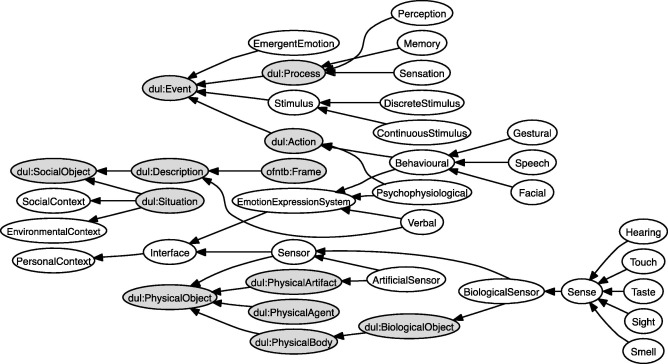
\includegraphics{upper_domain_interaction.jpg}
	\caption{An example of integrating a domain ontology
	(EmotionsOnto) with a upper ontology (DOLCE)
	Adopted from \citep{gil2015emotions}
	}
	\label{fig:upper_domain_integration}
\end{figure}

An upper ontology is a model of common relations and individuals that are generally
applicable across a wide range of domain ontologies. They usually have
a core glossary that contains terms and their decriptions of usage in various 
domain ontologies. Some popular upper ontologies are Dublin Core \citep{weibel1998dublin}, 
the suggested upper merged ontology SUMO \citep{pease2002suggested} and
DOLCE \citep{gangemi2002sweetening}. 
Upper ontologies are generally designed to be used with multiple domain ontologies. 
An example of an upper ontology integrated with a domain ontology is in 
figure~\ref{fig:upper_domain_integration}. 


% \begin{figure}
% 	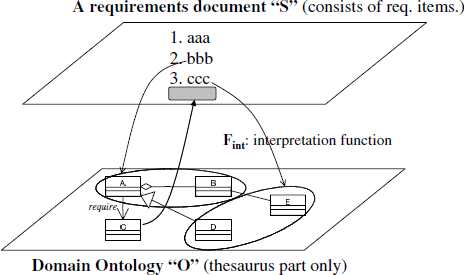
\includegraphics[scale=0.8]{ontology_creation.png}
% \end{figure}

Ontologies are often constructed from natural language requirements, 
such as ``a system can reserve seats in a specific train''. This sort of requirement can
then mapped to an ontological element ``reserve'' in the domain of 
reservation systems \citep{kaiya2006using}. 
Constructing a domain ontology often involves lexical decomposition
\citep{pustejovsky2013type} such that natural language requirements 
can be interpreted with ontological elements which can be decomposed 
into several unambiguous terms. The terms are often organized in a semantic structure,
a thesaurus of classes. Relationships between terms, relations, define how 
the terms are connected. 


% - (optional) joint modeling of sequence and classification \\
% 
% 


\part{Unstructured argumentation mining of claims}

\chapter{Claim Clustering}
\label{chap:argclu}

% TODO think about having an example with equivalent claims 
%expressed differently

We will start analyzing discussions by trying to find most prominent 
claims made in the discussion.
Users express claims to back up their opinion on a topic. 
Recongizing claims in text is a challenge in online discussions due to 
dealing with noisy, vague and implicit text. 
Found claims may represent the basis of
forming arguments. Arguments can then lead to more complex 
argumentation structures, such as argumentation schemes \citep{walton2008argumentation}. 
But, connecting claims and going beyond the claim level is
out of scope of this thesis. 

In this chapter, we will first investigate on how to find candidates of 
prominent claims from text, considering the variability on how 
claims can be expressed. Second, we investigate the possibility of 
acquiring prominent claims from an online discussion by means of clustering, 
setting a baseline for unsupervised prominent claim identification. 
We will start by introducing the dataset used to study clustering of
user comments to determine prominent claims in section~\ref{sec:argclu_data}.
Next, we will introduce an unsupervised
model for claim clustering in section~\ref{sec:argclu_model}.
The results of the model will be analyzed in section~\ref{sec:argclu_analysis}.
Finally, we will conclude in section~\ref{sec:argclu_conclusion}. 

\section{Data}
\label{sec:argclu_data}

We conduct our study on the dataset of users' posts compiled by \citet{hasan2014you}. 
The dataset is acquired from two-side online debate forums on four topics: 
``Obama'', ``Marijuana'', ``Gay rights'', and ``Abortion''.
Each post is assigned a stance label (\textit{pro} or \textit{con}), provided
by the author of the post. 
Furthermore, each post is split up into sentences and each sentence is manually labelled
with one prominent claim from a predefined set of prominent claims 
(different for each topic). 
All sentences are argumentative, non-argumentative sentences were removed from the 
dataset (ratio of argumentative sentences topically varies from  20\% to 43.7\%). 
\citet{hasan2014you} report high levels of inter-annotator agreement (between
0.61 and 0.67 $\kappa$). 
Additionally, sentences with rarely occuring prominent claims ($<2\%$) were removed. 
In the end, the dataset contains 3104 sentences (``Abortion'' 814, ``Gay rights'' 824, 
``Marijuana'' 836, and ``Obama'' 630) and 47 different prominent claims
(25 \textit{pro} and 22 \textit{con}, an average of 12 prominent claims per topic). 
Majority of sentences 2028 is labelled with \textit{pro} prominent claims. 
The average sentence length is 14 words. 

\section{Model}
\label{sec:argclu_model}

We use two approaches to measuring similarity of claims. 
%\paragraph{Vector space similarity. } 
We represent sentences as vectors in a semantic space. 
We use two represetations 
\begin{enumerate} 
\item a bag-of-word (BoW) vector, weighted
by inverse sentence frequency, and 
\item a distributed representation based on the skip-gram model
	\citep{mikolov2013distributed}. 
\end{enumerate}
These methods of representing sentences are explained in more detail in 
section~\ref{sec:word_representations}. 
We use BoW as it has been shown to be a powerful baseline for semantic similarity 
\citep{ramage2009random}. 
Using weighing by inverse sentence frequency is similar to the motivation 
of inverse-document frequency in tf-idf (described in section~\ref{sec:word_representations} and
equation~\ref{eq:idf}), which is that more frequently used words are less
specific to a prominent claim, thus contributing less to similarity. 
Distributed representations were chosen since they represent individual words 
very well (as shown in \citep{mikolov2013efficient, mikolov2013distributed}).
To build a sentence vector, we simply sum up the distributed vector representations 
of words\footnote{we use pretrained vectors from \url{https://code.google.com/archive/p/word2vec/}}
For both representations, we remove stopwords before building vectors. 
Similarity between sentences is computed as cosine similarity between 
respective sentence vectors. 
As described in section~\ref{sec:sts} we use TakeLab's STS, which we feed our pairs
of claims to acquire a similarity score. 

For clustering we use the hierarchical agglomerative clustering (HAC) algorithm
(described in section~\ref{sec:hierarhical_clustering}). 
There are three main reasons to use HAC: 
\begin{enumerate*}
\item HAC allows us to work directly with similarities
coming from the STS systems, instead of requiring explicit vector-space representations, 
\item HAC produces hierarhical structures, allowing to investigate
granularity of claims, and
\item HAC is a deterministic algorithm, making the results more stable.
\end{enumerate*}
HAC works with a distance matrix computed for all pairs of instances. 
We compute this matrix for all pairs of sentences $s_1$ and $s_2$ and 
compute vector-space similarity with: 
$$
\mathit{vs_{sim}} = 1 - \cos(v_1, v_2)
$$ 
where $v_1$ and $v_1$ are vectors for sentences $s_1$ and $s_2$ respectively.
STS similarity is computed as:
$$
\mathit{sts_{sim}} = \frac{1}{1 + \mathit{sim}(s_1, s_2)}
$$
where $\mathit{sim}(s_1, s_2)$ is a method that returns the STS similarity
between sentences $s_1$ and $s_2$. 
As for linkage, we use complete linkage and Ward's method \citep{ward1963hierarchical}. 
We do not cluster \textit{pro} and \textit{con} sentences separately. 
This allows us to investigate to which extent stance can be captured by 
semantic similarity (and is also more realistic). 

\section{Claim Cluster Analysis}
\label{sec:argclu_analysis}

- We perform two analysis \\
- first, we analyze different clustering models \\
- second, we analyze clustering quality \\

\begin{table*}[t]
\begin{center}
{\footnotesize
\setlength{\tabcolsep}{0.5em}
\begin{tabular}{@{}l cccc cccc cccc cccc@{}}
\toprule
& \multicolumn{4}{c}{``Obama''} & \multicolumn{4}{c}{``Marijuana''} & \multicolumn{4}{c}{``Gay rights''} & \multicolumn{4}{c}{``Abortion''} \\
\cmidrule(lr){2-5}
\cmidrule(lr){6-9}
\cmidrule(lr){10-13}
\cmidrule(lr){14-17}
Model (linkage) &
$h$ & $c$ & $V$ & ARI &
$h$ & $c$ & $V$ & ARI &
$h$ & $c$ & $V$ & ARI &
$h$ & $c$ & $V$ & ARI \\
\midrule
BoW (Complete) &
.15 & .15 & .15 & .03 & 
.04 & .04 & .04 & .00 & 
.04 & .04 & .04 & .01 & 
.05 & .04 & .04 & .01\\
%.153 & .150 & .152 & .025 & 
%.040 & .036 & .038 & .002 & 
%.039 & .036 & .038 & .007 & 
%.045 & .041 & .043 & .005\\
BoW (Ward's) & 
.22 & \textbf{.34} & .27 & .04 & 
.15 & .20 & .17 & .02 & 
.13 & \textbf{.17} & \textbf{.15} & .04 & 
.22 & \textbf{.27} & \textbf{.24} & .07 \\
%.218 & .342 & .266 & .042 & 
%.145 & .197 & .167 & .016 & 
%.127 & .169 & .145 & .038 & 
%.223 & .266 & .243 & .072 \\
Skip-gram (Complete) & 
.18 & .26 & .21 & .04 & 
.09 & .22 & .13 & .02 & 
.09 & .10 & .10 & .04 & 
.17 & .24 & .20 & .03  \\
%.177 & .261 & .211 & .041 & 
%.094 & .216 & .131 & .021 & 
%.089 & .104 & .096 & .043 & 
%.167 & .242 & .198 & .026  \\
Skip-gram (Ward's) & 
\textbf{.30} & .29 & \textbf{.30} & \textbf{.10} & 
\textbf{.25} & \textbf{.24} & \textbf{.25} & \textbf{.19} & 
\textbf{.16} & .15 & \textbf{.15} & \textbf{.07} & 
\textbf{.24} & .22 & .23 & \textbf{.08} \\
%.300 & .294 & .297 & .102 & 
%.250 & .242 & .246 & .186 & 
%.156 & .152 & .154 & .072 & 
%.235 & .217 & .226 & .078 \\
STS (Complete) & .11 & .11 & .11 & .02 & .05 & .05 & .05 & .03	& .05 & .05 & .05 & .01 & .06 & .06 & .06 & .02

 \\
\bottomrule
\end{tabular}}
\caption{External evaluation of clustering models on the four topics}
\label{tab:external-eval}
\end{center}
\end{table*}

\noindent - to evaluate, we adopt the external evaluation approach, which compares the 
hypothesized clusters against target clusters \\
- we use argument labels from \citet{hasan2014you} as target clusters \\
- to measure, we use two measures: adjusted rand index (ARI) 
\citep{steinley2004properties}, and V-measure \citep{rosenberg2007v}
(methods described in section~\ref{sec:clus_evaluation}, more specifically by equations
~\ref{eq:adjusted_rand_index} and~\ref{eq:v-measure})
\\

\noindent \textbf{Analysis 1} - we cluster sentences from four topics separately \\
- we use the gold number of clusters for each topic \\
- results are shown in table~\ref{tab:external-eval} \\
- overall, the best model is skip-gram with Ward's linkage 
outperforming in both ARI and V-measure \\
- it also produces best clusters in terms of homogeneity and 
completeness \\
- Ward's linkage seems to work better than complete for both BoW and skip-gram
- STS behaves comparable to baseline results \\
- the reason in poor performance might lie in the fact that STS was trained 
on different domains, and does not model the claim similarity we seek here 
% TODO (not sure  if I should put this given the next chapter)
- there is a lot of variance across different topics \\
- claims from ``Gay rights'' seem most difficult to cluster, whereas 
``Marijuana'' seems to be the easiest \\
- in subsequent experiments, we focus on the skip-gram model 
with Ward's linkage and the ``Marijuana'' topic \\

\begin{table*}
\setlength{\tabcolsep}{0.4em}
{\scriptsize
\begin{center}
\begin{tabular}{lp{3.8em}p{33.0em}|lp{3.8em}p{10em}}
\toprule
\multicolumn{3}{c}{Hypothesized clustering} & \multicolumn{3}{c}{Gold classes}\\
\cmidrule(lr){1-3}\cmidrule(lr){4-6}
Id & Classes & Cluster medoid & Id & Clusters & Gold argument \\
\midrule
1 &  \textbf{10 (54\%)}  \newline  2 (12\%)  \newline  6 (10\%)  &

\str{%
Tobacco and alcohol are both legal and widely used in the US, (...) If the abuse of marijuana is harmful, isn't the abuse of tobacco or alcohol equally life threatening? (...)
} &

1  &  5 (23\%) \newline 9 (19\%) \newline 10 (18\%) 
&
\str{%
%I would argue that marijuana should be illegal as long as all other drugs are illegal, but then again, marijuana has actually treated people with anorexia and helped other people with loss of appetite.
Used as a medicine for its positive effects
}
\\
\midrule
2 & \textbf{4 (92\%) } \newline  9 (8\%) &
\str{%
The biggest effect would be an end to brutal mandatory sentencing of long jail times that has ruined so many young peoples lives.
} 
& 
2  &  1 (33\%) \newline 9 (28\%) \newline 3 (15\%) 
&
\str{%
%(...) I think it ridiculous that people want to legalise something that has four - seven times the amount of tar (the cancer causing agent) in one cone than in one cigarette (...)
Responsible for brain damage
}

\\
\midrule
3 &  \textbf{9 (44\%)}  \newline  4 (25\%)  \newline 7 (8\%) &
\str{%
Legalizing pot alone would not end the war on drugs. It would help (...) my personal opinion would be the only way to completely end the war on drugs would be to legalize everything. 
} 
& 3  &  9 (41\%) \newline 3 (23\%) \newline 10 (23\%) 
&
\str{%
%Worst case scenario, half the population would go out and buy it, get high and wreak havoc on America. Productivity would go down :) and some people would simply do reckless things.
Causes crime
}

\\
\midrule
4 &  \textbf{8 (37\%)}  \newline  1 (22\%)  \newline  10 (17\%)   & 
\str{%
What all these effects have in common is that they result from changes in the brain's control centers (...) So, when marijuana disturbs functions centered in the deep control centers, disorienting changes in the mind occur (...)
} &
4  &  9 (40\%) \newline 3 (26\%) \newline 10 (12\%)  
&
\str{%
%it is not the governments place to control personal aspects of my life that would have no affect on anyone else.
Prohibition violates human rights
}
\\
\midrule
5 &  \textbf{1 (45\%)}  \newline  6 (18\%)  \newline  8 (10\%)  & 
\str{%
People with pre-existing mental disorders also tend to abuse alcohol and tobacco. (...) the link between marijuana use and mental illness may be an instance when correlation does not equal causation. 
} 
&
5  &  6 (25\%) \newline 7 (25\%) \newline 4 (18\%) 
&
\str{%
%you also have to consider that continuous usage of LSD can cause severe mental illnesses in people. There hasn't ever been a case of this happening from using marijuana.
Does not cause any damage to our bodies
}
\\
\midrule
6 &  \textbf{5 (63\%)}  \newline  10 (31\%)  \newline  1 (6\%) & 
\str{%
There are thousands of deaths every year from tobacco and alcohol, yet there has never been a recorded death due to marijuana.
} &
6  &  9 (29\%) \newline 1 (19\%) \newline 7 (16\%) 
&
\str{%
%There have been many deaths directly linked to marijuana use. Car crashes are a common way in which people under the influence of marijuana harm themselves, and others.
Damages our bodies
}
\\
\midrule
7 &  \textbf{10 (48\%)}  \newline  5 (13\%)  \newline  6 (12\%)    &
\str{%
as far as it goes for medicinal purposes, marijuana does not cure anything (...) It is for the sole purpose of numbing the pain in cancer patients (...) and also making patients hungry so they eat more and gain weight on their sick bodies 
} &
7  &  9 (39\%) \newline 3 (30\%) \newline 1 (9\%) 
&
\str{%
%The last thing we need is more people doing it. More people making it a problem for themselves, more people ending up in rehab at the governments expense.
Highly addictive
}
\\
\midrule
8 &  \textbf{9 (92\%)} &
\str{%
the economy would get billions of dollars in a new industry if it were legalized (...) no longer would this revenue go directly into the black market.
} 
&
8  &  4 (44\%) \newline 7 (16\%) \newline 9 (16\%) 
&
\str{%
%If we legalize something that makes people stop caring about their lives and only want to get "high" then we are pretty much setting a course for our downfall as a civilization.
If legalized, people will use marijuana and other drugs more
}
\\
\midrule
9 &  \textbf{4 (30\%)}  \newline  9 (13\%)  \newline  10 (11\%)   &
\str{%
(...) I think it ridiculous that people want to legalise something that has four - seven times the amount of tar (the cancer causing agent) in one cone than in one cigarette (...)
} &
9  &  8 (53\%) \newline 3 (25\%) \newline 9 (10\%) 
&
\str{%
%Not only would it be better for the economy, but look at Amsterdam - weed is legal over there and you never hear anything out of them. They've been onto something for a long time now.
Legalized marijuana can be controlled and regulated by the government
}
\\
\midrule
10 &  \textbf{10 (30\%)}  \newline  9 (19\%)  \newline  4 (15\%)   &
\str{%
But I'm not gonna tell anyone they can't smoke pot or do meth because I don't like it.
} &
10  &  1 (36\%) \newline 7 (21\%) \newline 10 (18\%) 
& 
\str{%
%I don't personally use it, or have any real want to, but I don't think it's any worse than alcohol or cigarettes.
Not addictive
}
 \\
\bottomrule
\end{tabular}
\caption{Manual cluster-class matching for the ``Marijuana'' topic and the gold number of clusters}
\label{tab:cluster-class}
\end{center}}
\end{table*}

\begin{table*}
\setlength{\tabcolsep}{0.4em}
{\scriptsize
\begin{center}
\begin{tabular}{@{}lp{19em} p{16em} p{16em}@{}}
\toprule
Id & Statement & Hypothesized clustering argument & Gold argument \\
\midrule
\#knowledge  & 
\str{%
Pot is also one of the most high priced exports of Central American Countries and the Carribean}
& 
\str{%
Not addictive
}
& 
\str{%
Legalized marijuana can be controlled and regulated by the government} 
\\
\midrule
\#colloquial & 
\str{%
If I want to use pot, that is my business!}
& 
\str{%
Legalized marijuana can be controlled and regulated by the government} &
\str{%
Prohibition violates human rights}
\\
\midrule
\#opposing & 
\str{%
(...) immediately following the legalization of the drug would cause widespread pandemonium. (...)
} 
& 
\str{%
Legalized marijuana can be controlled and regulated by the government
} & 
\str{%
If legalized, people will use marijuana and other drugs more }
\\
\midrule
\#general & 
\str{%
The user's psychomotor coordination becomes impaired (...), narrow attention span, "depersonalization, euphoria or depression (...)
}
& 
\str{%
Damages our bodies
}
& 
\str{%
Responsible for brain damage
} 
\\
%3 & 
%\str{%
%You're right that not many people ask where their stuff is from but even the dealer has a duty to the buyer to expose a heavy additive
%}
% & 
%\str{%
%Prohibition violates human rights
%} &
%\str{%
% Highly addictive} 
%  \\
%\#specific & 
%\str{%
%People who are already obese would get the munchies and that would make matters worse.
%} &
%\str{%
%If legalized, people will use marijuana and other drugs more.
%} &
%\str{%
%Highly addictive
%}
%\\
%10  & 
%\str{%
%Sure it makes you sleepy and hungry but it also makes you happy!} & 
%\str{%
%Used as a medicine for its positive effects}
%& \str{%
%Does not cause any damage to our bodies}
%\\
%\#rhetorical & 
%\str{%
%Who are you to tell me what I ingest?   If I want to snort cocaine, why can't I?} &
%\str{%
%Legalized marijuana can be controlled and regulated by the government
% }
% & 
% \str{%
% Prohibition violates human rights
% }
% \\
\bottomrule
\end{tabular}
\caption{Error analysis examples for the ``Marijuana'' topic}
\label{tab:err-analysis}
\end{center}}
\end{table*}

\noindent \textbf{Analysis 2} - cluster-class matching \\
- we manually attempt to match resulting clusters from 
the skip-gram model with Ward's linkage for the ``Marijuana'' topic \\
- there is 10 gold clusters 
we do matching on the majority basis, which matches 6 gold classes \\
- results are shown in table~\ref{tab:cluster-class} \\
- we list top three gold classes (and the percentage of sentences in the dataset) 
in each predicted cluster and top three
(and the percentage of sentences) in each of the gold classes \\
- two gold classes  ($\#4$ and $\#9$) frequently co-occur, indicating 
that they are similar \\
- we characterize each cluster by its medoid (the sentence closest to cluster centroid)
\\

\noindent \textbf{Error analysis} \\
- grouping statements into coherent clusters is challenging \\
- we notice that the main problems are related to \begin{enumerate*}
\item need for background knowledge, 
\item use of idiomatic language, 
\item grammatical errors, 
\item opposing claims, and 
\item too fine/coarse gold claims.
\end{enumerate*} \\
- we show sample errors in table~\ref{tab:err-analysis} \\
- Ex \#knowledge demonstrates the need for background knowledge 
(exports are government regulared) \\
- a colloquial expression (pot) is used in example \#colloquial \\
- in \#oppose, the statement is assigned to cluster of the opposite-stance
claim \\
- in ex. \#general our model predicts are more coarse claim \\

\begin{figure}
\begin{center}
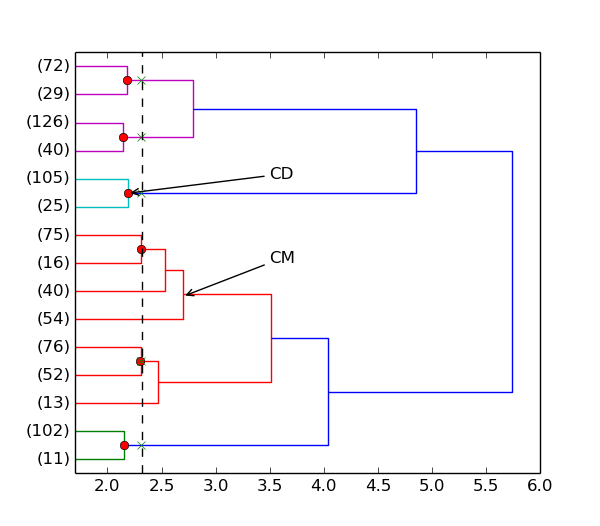
\includegraphics{dendrogram.png}
\end{center}
\caption{Dendrogram for applying HAC (last 15 steps) on the ``Marijuana'' topic.
The dashed line shows the 10-clusters cut, which is number of gold prominent
claims. \\
CM denotes a merger of clusters that consist mostly of two prominent claims: 
\textit{Damages our bodies} and \textit{Responsible for brain damage}.  \\
In CD there is a split between clusters represented by medoids with: 
item \textit{the economy would get billions of dollars (...) no longerwould this revenue
go directly into the black market} and 
\textit{If the tax on cigarettes can
be \$5.00/pack imagine what we could tax pot for!}
}
\label{fig:dendrogram}
\end{figure}

\noindent - in the previous analysis we used the gold number of prominent claims to compare
against \\
- however, we note that claim granularity is something arbitrary \\
- we exemplify this with example~\ref{fig:dendrogram} where the last 15 HAC steps \\
- In CD there is a split between clusters represented by medoids with: 
\begin{enumerate*}[label=\arabic*)]
\item \textit{the economy would get billions of dollars (...) no longerwould this revenue
go directly into the black market} and 
\item \textit{If the tax on cigarettes can
be \$5.00/pack imagine what we could tax pot for!}
\end{enumerate*}\\
- these could be treated as separate prominent claims about economy and tax \\
- On the other hand,  CM denotes a merger of clusters that consist mostly of two prominent claims: 
\begin{enumerate*}[label=\arabic*)]
\item \textit{Damages our bodies} and 
\item \textit{Responsible for brain damage}.
\end{enumerate*}  \\
- these could be represented as a single prominent claim which would state: 
\textit{Damaging our entire bodies} \\
- the dendrogram also suggests that having 10 prominent claims might not be optimal 
for the ``Marijuana'' topic and the similarity measure used \\

\section{Conclusion}
\label{sec:argclu_conclusion}

- this work is about unsupervised identification of prominent claims in online 
discussions \\
- hierarchical clustering (HAC) is used to cluster semantically similar sentences from 
discussions \\
- best performing model achieved 0.15 to 0.30 V-measure \\
- there seem to be differences that basic textual similarity can't measure, as it might be
too surface level \\
- identifying prominent claims from text might be an extremely difficult problem using 
such methodologies \\
- we will revisit this and suggest different approaches in 
%TODO add future reference of revisiting this problem altogether 
- now a transition to do argument recognition \\


%TODO think about the naming
\chapter{Prominent Claim Identification}
\label{chap:argrec}

Prominent claim identification aims to determine which claims are predominately
used to express and base users' stance on. The task of prominent claim
identification has also been reffered to as \textit{argument-based opinion mining}
\citep{boltuzic2014back}, reason classification \citep{hasan2014you}, and
argument tagging \citep{sobhani2015argumentation}. 
The problem of prominent claim identification involves determining
the relationship between a comment a set of well-established prominent claims. 
Consider a discussion on the topic ``\emph{Should gay marriage be legal}''
and a following comment: 
\begin{quote}
\emph{
Gay marriages must be legal in all 50 states. A marriage is covenant
between 2 people regardless of their genders. Discrimination against
gay marriage is unconstitutional and biased. Tolerance,education and
social justice make our world a better place.
}
\end{quote}
This comment supports the claim ``\emph{It is discriminatory to refuse
gay couples the right to marry}'' and attacks the claim
``\emph{Marriage should be between a man and a woman}''. 
The technical challenge here lies in the fact that, unlike
in debates or other more formal, argumentation sources, 
claims provided by users are usually less formal, ambiguous, vague, 
implicit, or often simply poorly worded. 
The task of \textbf{prominent claim identification} is defined 
as identifying what prominent claims, from a predefined set of prominent claims, 
have been used in users' comments, and how. 
A topic-dependent set of prominent claims is assumed to exist. 
Users' comments typically contain more than one claim, but in their 
own wording and with varying degree of explicitness. 
The task of prominent claim identification amounts to matching
users' comments to prominent claims, which can be either attack or 
supported by the comment. 
The user comment may be a single prominent claim (and it often is), but it 
is reffered to as a \textit{comment} to emphasize the fact that in general 
it may contain several claims, as well as non-argumentative text. 

In this chapter, we first introduce the \ComArg corpus in section~\ref{sec:comarg}
which contains labelled pairs of comments with prominent claims. Next, 
we build a model for prominent claim identification as described in 
section~\ref{sec:argrec_model}. The model is evaluated in 
section~\ref{sec:argrec_experiments}. Finally, we conclude in 
section~\ref{sec:argrec_conclusion}.

\begin{table}
\centering
{\small
\begin{tabular}{cl}
\toprule
Label & Description: Comment\dots \\
\midrule
\textbf{A} & \dots explicitly \textbf{attacks} the prominent claim \\
\textbf{a} & \dots vaguely/implicitly \textbf{attacks} the prominent claim \\
\textbf{N} & \dots makes \textbf{no use} of the prominent claim \\
\textbf{s} & \dots vaguely/implicitly \textbf{supports} the prominent claim \\
\textbf{S} & \dots explicitly \textbf{supports} the prominent claim \\
\bottomrule
\end{tabular}
}
\caption{Labels for comment-prominent claim pairs in the \ComArg corpus}
\label{tab:comarg-labels}
\end{table}

\section{\ComArg corpus}
\label{sec:comarg}

For training and evaluatiing prominent claim identification models, 
we have compiled a corpus of user comments, manually annotated
with prominent claims which we refer to as \ComArg. \ComArg is
freely available\footnote{Freely available under the CC BY-SA-NC license from
\url{http://takelab.fer.hr/data/comarg}}. 
As a source of data we use two websites:
\emph{procon.org}\footnote{\url{http://www.procon.org}} and 
\textit{idebate.org}.\footnote{\url{http://idebate.org}}. 
The former is a discussion site covering ideological, social, political, and
other topics where users express their personal opinions on a selected topic,
taking either the \textit{pro} or \textit{con} side.  The latter,
\textit{idebate.org} is a debating website containing online debates and an
archive of past debates.  Each archived topic contains a set of prominent
claims presented in the debate.  Each claim is labelled as either \textbf{for}
or \textbf{against} the topic The claims are moderated and edited to provide
the best quality of information. 

The two datasources are complementary to each other as \textit{procon.org}
contains user comments, while \textit{idebate.org} contains prominent claims. 
We manually identified near-identical topics covered by both web sites. 
We choose two topics: ``\textit{Under God in Pledge}'' (UGIP) and 
``\textit{Gay marriage}'' (GM), since
they have a larger-than-average number of comments (above 300) and are 
well-balanced between \textbf{pro} and \textbf{con} stances. 
For these two topics, we then took the corresponding comments and prominent claims
from \textit{procon.org} and \textit{idebate.org} respectively. 
As the users can produce comments not relevant to the topic, we skim-read 
the comments and omit non-argumentative comments.  We end up with a set of 175
comments and 6 arguments for UGIP, and 198 comments and 7 arguments for the GM
topic. 
The comments are often verbose: the average number of words per comment is 116. 
Each comment has an associated stance (\textbf{pro} or \textbf{con}) depending on 
how it was classified in \textit{procon.org}. 
Similarly, each prominent claim either attacks or supports the claim of the topic,
depending on how it was classified on \textit{idebate.org}, these claims will be reffered to 
as ``pro prominent claims'' and ``con prominent claims''. 
Table~\ref{tab:comarg-claims} shows prominent claims for ``\emph{Under god in Pledge}
and ``\textit{Gay marriage}'' topics. 

\begin{table}[t]
%\setlength{\tabcolsep}{5.5pt}
\centering
{\small
\begin{tabular}{lp{12cm}l}
\toprule
& Prominent claim & Pro/Con\\
\midrule
\multicolumn{3}{p{13cm}}{\textbf{``Under God in Pledge'' (UGIP):} \emph{Should
the words ``under God'' be in the U.S. Pledge of Allegiance? }}\\
%\multicolumn{3}{p{13cm}}{\textit{``under God'' be in the U.S. Pledge of Allegiance?}}\\
(A1.1) & \normalsize{Likely to be seen as a state sanctioned condemnation of religion}  &  Pro \\
(A1.2) & \normalsize{The principles of democracy regulate that the wishes of American Christians,
     who are a majority are honored} & Pro \\
(A1.3) & \normalsize{Under God is part of American tradition and history} & Pro  \\  
(A1.4) & \normalsize{Implies ultimate power on the part of the state} &   Con \\  
(A1.5) & \normalsize{Removing under god would promote religious tolerance} & Con \\  
(A1.6) & \normalsize{Separation of state and religion} & Con \\
\midrule
\multicolumn{3}{l}{\textbf{``Gay Marriage'' (GM):} \emph{Should gay marriage be legal?}}\\
(A2.1) & \normalsize{It is discriminatory to refuse gay couples the right to marry} & Pro \\
(A2.2) & \normalsize{Gay couples should be able to take advantage of the fiscal and legal
benefits of marriage} & Pro \\
(A2.3) & \normalsize{Marriage is about more than procreation, therefore gay couples should not 
be denied the right to marry due to their biology} & Pro\\
(A2.4) & \normalsize{Gay couples can declare their union without resort to marriage} & Con \\
(A2.5) & \normalsize{Gay marriage undermines the institution of marriage, leading to an increase
in out of wedlock births and divorce rates} & Con \\
(A2.6) & \normalsize{Major world religions are against gay marriages} & Con \\
(A2.7) & \normalsize{Marriage should be between a man and a woman} & Con \\
\bottomrule
\end{tabular}
}
\caption{Predefined prominent claims for the two topics in the \ComArg corpus}
\label{tab:comarg-claims}
\end{table}

Users may attack or support both \textbf{pro} and \textbf{con} arguments. 
We will refer to the way how the argument is \textit{used} (attacked or supported)
as prominent claim polarity. 
Typically, users who take the \textbf{pro} stance do so by supporting one of the \textbf{pro}
prominent claims, and perhaps attacking some of the \textbf{con} prominent claims, while
for users who take the \textbf{con} stance it is the other way around. 

%\subsection{Annotation}

Annotation is done by labelling the prominent claims and polarity  
used in each comment. 
We paired all comments with all possible prominent claims for the topic , resulting in
1,050 and 1,386 comment-prominent claim pairs for the ``\emph{Under God
in pledge}'' and ``\emph{Gay marriage}'' topics, respectively. 
We then ask annotators to annotate each prominent claim--coment pair.\footnote{we 
initially attempted to crowdsource the annotation with guidelines listed in 
appendix~\ref{sec:argrec_annotation}. We used the same guidelines with expert annotators
to much greater success.}
Since user-provided claims (in comments) are often vague or implicit, we therefore decided to
annotate each comment-prominent claim using a five point scale shown in 
table~\ref{tab:comarg-labels}. Labels encode the presence (\textbf{A, a, s, S})
or absence (\textbf{N}) of a prominent claim in a comment, its polarity
(comment labelled \textbf{S} and \textbf{s} supports the prominent claim; comment labelled
\text{A} and \text{a} attacks the prominent claim),
as well as degree of 
explicitness (\textbf{A} expresses attacking more explicitly than \textbf{a};
\textbf{S} expresses support
more explicitly than \textbf{s}). 

\begin{table}
\centering
{\small
\begin{tabular}{lrrrrrr}
\toprule
& \multicolumn{5}{c}{Labels}\\
\cmidrule(lr){2-6}
Topic & \textbf{A} & \textbf{a} & \textbf{N} & \textbf{s} & \textbf{S} & Total \\
\midrule
UGIP         & 48  & 86 & 691 & 58 & 130 & 1,013 \\
GM           & 89 & 73 & 849 & 98 & 176 & 1,285 \\
UGIP+GM      & 137 & 159 &1,540 & 156& 306 & 2,298 \\
\bottomrule
\end{tabular}
}
\caption{Distribution of labels in the \ComArg corpus}
\label{tab:labels}
\end{table}

\begin{table}
\centering
{\small
\begin{tabular}{@{}p{\columnwidth}@{}}
\toprule
\textit{
\normalsize{%
No, of course not. The original one was good enough.  The insertion of Under
God" between "Our nation" and "indivisible" is symbolic of how religion divides
this country."}
}\\
\midrule
\normalsize{%
\textit{
The Pledge of Allegiance reflects our morals and values. Therefore, it should
reflect the ideas of all Americans not 80\%. This country has no national
religion, so why should we promote a god. Also, Thomas Jefferson, a founding
father, was athiest.
}
}
\\
\midrule
\normalsize{%
\textit{
I believe that since this country was founded under God why should we take that
out of the pledge? Men and women have fought and gave their lives for this
country, so that way we can have freedom and be able to have God in our lives.
And since this country was founded under God and the Ten Commandments in mind,
it needs to stay in. If it offends you well I am sorry but get out of this
country!}
}\\
\bottomrule
\end{tabular}
}
\caption{Example comments with low IAA from UGIP}
\label{tab:problematic-comments}
\end{table}

The annotatation was carried out by three trained annotators, in two
steps. 
In the first step, each annotator indepedently annotated the complete dataset
of 2,436 comment-prominent claim pairs. 
To improve annotation quality, we single out the problematic comment-prominent claim
pairs. 
Pairs were deemed problematic if 
\begin{enumerate*} 
\item there is no agreement among three annotators or
\item the ordinal distance between any of the labels assigned
by the annotators is greater than one. 
\end{enumerate*}
Table~\ref{tab:problematic-comments} shows some examples of problematic comments. 
Most problematic prominent claims are \textit{A1.3} and \textit{A1.5} for the 
``\emph{Under God in pledge}'' topic
and prominent claims \textit{A2.1} and \textit{A2.7} for the ``\emph{Gay marriage}''
topic (references
in table~\ref{tab:comarg-claims}). 
In the second step, we asked annotators to indepedently revise 
their decisions for the problematic comment-prominent claim pairs. 
Each re-annotated 515 pairs of which 86 were revised. 
The annotation took around 30 person-hours. 

Table~\ref{tab:iaa} shows interannotator agreement (IAA). 
We compute Fleiss' multirater kappa, Cohen's kappa (denoted as $\kappa$, calculated by
averaging over three annotator pairs), Cohen's linearly weighted kappa (also
averaged) and Pearson's \textit{r}.
The latter two reflect the fact that the five labels constitute an ordinal scale. 
According to standard interpretation \citep{landis1977measurement} resulting
values ($\kappa = 0.49$) indicate moderate agreement 
To obtain gold standard annotation, we took the majority label for 
each comment-prominent claim pair, discarding the pairs with ties. 
We ended up with a dataset of 2,249 comment-prominent claim pairs. 
Table~\ref{tab:comarg} shows examples of annotated pairs. 

\begin{table}
\centering
{\small
\begin{tabular}{l ccc}
\toprule
%& \multicolumn{2}{c}{A-a-N-s-S} & \multicolumn{2}{c}{Aa-N-sS} &
%\multicolumn{2}{c}{A-N-S}\\
%\cmidrule(lr){2-3}\cmidrule(lr){4-5}\cmidrule(lr){6-7}
IAA & UGIP & GM & UGIP+GM \\
\midrule
Fleiss' Kappa    & 0.46 & 0.51 & 0.49 \\
Cohen's Kappa    & 0.46 & 0.51 & 0.49 \\
Weighted Kappa   & 0.45 & 0.51 &  0.50\\
Pearson's $r$    & 0.68 & 0.74 &  0.71 \\
\bottomrule
\end{tabular}}
\caption{Interannotator agreement on the \ComArg corpus}
\label{tab:iaa}
\end{table}

% \subsubsection{Annotation analysis}

Table~\ref{tab:labels} shows distribution of labels across pairs. 
Majority (67.0~\%) of pairs are the cases in which the argument is not used
(label \textbf{N}).
Attacked arguments (labels \textbf{A} or \textbf{a}) make up 12.9\% while supported
arguments (labels \textbf{S} or \textbf{s}) make up 20.1\%
Among the cases not labelled as \textbf{N}, prominent claims are used explicitly 
in 58.4\% (labels \textbf{A} and \textbf{S}) and vague/implicit (labels \textbf{a} and \textbf{s})
in 41.5\% of cases. 
There is a difference across topics: in ``\emph{Under God in Pledge}''
prominent claims are explicit in 55.3\%, while in 
``\emph{Gay Marriage}'' in 60.7\% of cases. 
There might be an effect on how the choice of predefined prominent claims along with their 
wording.  
The average number of prominent claims in a comment is $1.9$ ($1.8$ for 
``\emph{Under God in Pledge}'', $2.0$ for ``\emph{Gay Marriage}''). 
In ``\emph{Under God in Pledge}'', 62.8\% prominent claims are \textbf{pro},
while in ``\emph{Gay Marriage}'' \textbf{pro} claims 
make up 52.2\% cases. 

\begin{table}[t!]
{\small
\begin{tabular}{@{}lp{9.5cm}p{3.5cm}c@{}}
\toprule
Id & Comment & Argument & Label \\
%1.102.1 & \normalsize{%
%I'm a cathloic but after reading the history I believe We are trampling upon the 1st amendment.}
%& \normalsize{%
%Separation of state and religion.}
%& S \\
%\midrule
%2.107.1 & \normalsize{%
%As pluralistic nation, there are a large number of different gods.  Who is to
%say is The" God.  Or there may not even be a god of any kind.  As atheists and
%many agnostics say there is no justification to believe there is one or many
%gods.  The phrase "under God" does not reflect the idea of one nation, it
%reflects the coercion of one religion to impose their beliefs on all, that is
%immoral."}
%& \normalsize{%
%Separation of state and religion.}
%& N \\
\midrule
2.23.4 & \normalsize{%
\textit{
All these arguments on my left are and have always been FALSE. Marriage is
between a MAN and a WOMAN by divine definition. Sorry but, end of story.
}}

& \normalsize{%
\textit{ It is discriminatory to refuse gay couples the right to marry.}
}
& \textbf{s} \\
%\midrule
%1.139.3 & \normalsize{%
%(...) Whether some people like it or not there is no denying
%that the founding of our country was majorly based on a belief in God and
%relying on Him for help and guidance. And the separation of Church and State is
%actually not in the Constitution but in a letter that Thomas Jefferson wrote to
%a church to reassure them that the GOVERNMENT couldn't make laws about the
%CHURCH not that the Church couldn't be involved in the Government. There is a
%difference.}
%& \normalsize{%
%Under God is part of American tradition and history.}
%& S \\
%\midrule
%1.80.3 & \normalsize{%
%Yes because the united states was found under the christian religion.}
%& \normalsize{%
%Under God is part of American tradition and history.}
%& \alert{S} \\
\midrule
2.111.4 & \normalsize{%
\textit{
Marriage isn't the joining of two people who have intentions of raising
and nurturing children. It never has been. There have been many married couples
whos have not had children. (\dots) If straight couples can attempt to work out a
marriage, why can't homosexual couple have this same privilege? (\dots)
}} 
& \normalsize{%
\textit{
It is discriminatory to refuse gay couples the right to marry
}
}
& \textbf{s} \\
\midrule
2.114.2 & \normalsize{%
\textit{
(\dots) I truly believe that the powers
behind the cause to re-define marriage stem from a stronger desire to attack a
religious institution that does not support homosexuality, rather than a desire
to achieve the same benefits as marriage for same sex couples. (\dots)''} 
}
& \normalsize{%
\textit{
Gay couples should be able to take advantage of the fiscal and legal benefits
of marriage.} 
}
& \textbf{S} \\
\midrule
2.101.2
&
\normalsize{%
\textit{
(\dots) One part of marriage is getting benefits from the other. Many married
couples never have children but still get the benefits of marriage, should we
take those benefits away because they don't have children? Another is the
promise to be with each other for an eternity" etc. Marriage is also about
being able to celebrate having each other. And last, marriage is about being
there for each other. (\dots)''
}
}
&
\normalsize{%
\textit{
Gay couples should be able to take advantage of the fiscal and legal benefits
of marriage.
}
}
& \textbf{S} \\
\midrule
2.157.2 & \normalsize{%
\textit{
(\dots) There are no legal reasons why two homosexual people should not be
allowed to marry, only religious ones (\dots)
}
} & \normalsize{%
\textit{
Gay couples should be able to take advantage of the fiscal and legal benefits
of marriage.
}
} & \textbf{N} \\
\midrule
1.45.2 & \normalsize{%
\textit{
 I am not bothered by under God but by the highfalutin christians that do not
 realize that phrase was never in the original pledge - it was not added until
 1954. So stop being so pompous and do not offend my parents and grandparents
 who never used ``under God'' when they said the pledge. Let it stay, but know
 the history of the Cold War and fear of communism.
 }} & 
 \normalsize{
 \textit{
 ``Under God'' is part of American tradition and history.
 }} & \textbf{a}  \\
\bottomrule
\end{tabular}
}
\caption{Example of comment-prominent claim pair annotations from the \ComArg corpus}
\label{tab:comarg}
\end{table}


\section{Model}
\label{sec:argrec_model}

We cast the prominent claim identification problem as a multiclass problem
(multiclass problems described in section~\ref{sec:unstruc_machine_learning}). 
Given a comment-prominent claim pair as input, the classifier should
predict the correct label from the set of five possible labels (labels
listed in table~\ref{tab:labels}). 
The classifier should rely on the features derived from the comparison
of the comment and prominent claim. 
This approach, ideally, should be less domain-dependent than using features
directly from the comment or prominent claim. 
Three kinds of features are used: \begin{enumerate*}
\item textual entailment (TE) features, 
\item semantic text similarity (STS) features, and
\item ``stance alignment'' (SA) features. 
\end{enumerate*}
Textual entailment is described in section~\ref{sec:textual_entailment}, whereas
semantic textual similarity is described in section~\ref{sec:sts}, 
``stance alignment'' is a binary feature whose value is set to one if a
\textbf{pro} comment is paired with a \textbf{pro} prominent claim or if a
\textbf{con} comment is paired with a \textbf{con} prominent claim.  This SA
feature presupposes that comment stance is known a priori.

\begin{figure}
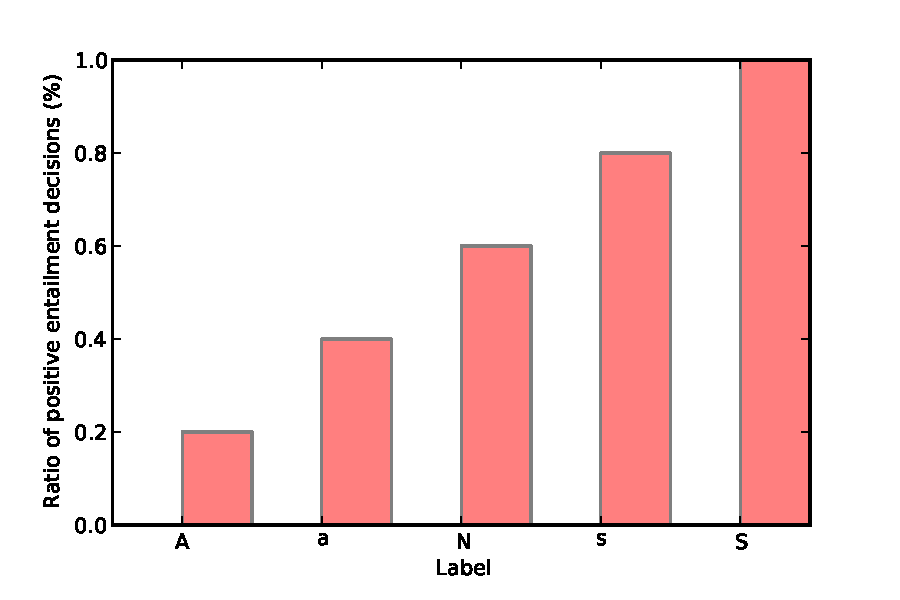
\includegraphics{entailment.pdf}
\caption{Ratio of positive entailment decisions across labels, scaled to a $[0,1]$ interval
}
\label{fig:entailment_ratio}
\end{figure}

% entailment
Following the work of \citet{cabrio2012combining}, we use textual 
entailment to determine whether the comment (text) entails the prominent
claim (hypothesis). 
To this end, we use the Excitement Open Platform (EOP) \citep{pado2015design}. 
From EOP, we used seven pre-trained \textit{entailment decision algorithms}
(EDAs). 
Some EDAs use only syntactical features, whereas others rely on
WordNet \citep{miller1995wordnet}, VerbOcean \citep{chklovski2004verbocean}. 
Each EDA outputs a binary decision (\textit{Entailment} or \textit{NonEntailment})
along with a degree of confidence. 
We use all seven (decisions and confidences) of EDAs as features for our classifier 
(14 features in total). 
We experiment with additional features (the disjunction of all classifier decisions, 
max of seven EDA confidence values, mean value of seven EDA confidences), but those
did not impact performance. 
The motivation for this set of features is that we expect the comment text
(usually longer and specific) to entail the prominent claim (usually shorter
and more general).
This intuition is confirmed in figure~\ref{fig:entailment_ratio}
where it shown that 
pro prominent claims have a higher ratio of positive entailment decisions than
con prominent claims.
Also vaguely supported prominent claims have a lower rate of entailment
decisions than explicitly supported prominent claims. 

\begin{figure}
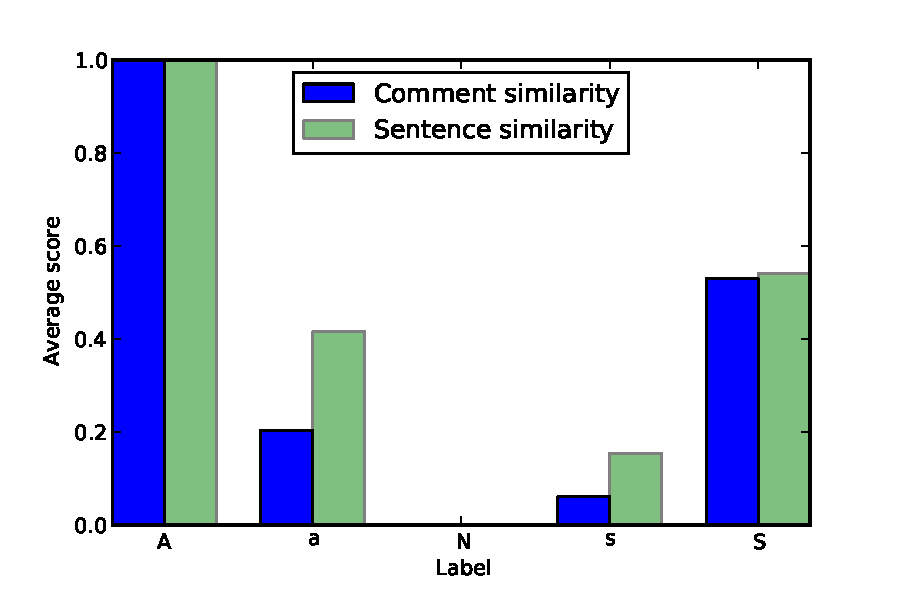
\includegraphics{similarity.pdf}
\caption{Average similarity score  on sentence and comment level across
labels, scaled to a $[0,1]$ interval}
\label{fig:sts_comarg}
\end{figure}

% semantic textual similarity
The prominent claim should either be entailed or not entailed from the comment. 
The former case also includes a paraphrase. 
In the latter case, there might be a contradiction or it may be \textit{non sequitur}. 
These relations can be hard to detect, especially from vaguely stated comments. 
To account for this, we use a feature based on semantic textual similarity (STS). 
We use TakeLab's STS \citep{vsaric2012takelab} which works as described in
section~\ref{sec:sts} to get a similarity score between 
a comment and a prominent claim, as well as the similarity score between 
each sentence of the comment and the prominent claim. 
Thus we have a vector of similarities (one global, one for each sentence) of size
29 (which is the max number of sentences in \ComArg ). 
We also use the mean of sentence-level similarities, ending up with a total of 31 STS features. 
Figure~\ref{fig:sts_comarg} shows the average comment- and sentence-level similarity scores
across labels on \ComArg scaled to a $[0, 1]$ interval.
Interestingly, attacked prominent claims receive a larger score than supported
arguments. 

\section{Experimental Evaluation}
\label{sec:argrec_experiments}

We consider three formulations of the prominent claim identification task. 
In the first setting (\textbf{A-a-N-s-S}), we consider classification of a comment-prominent claim
into one of the five labels, i.e. wish to determine whether a prominent claim was used, 
its polarity and degree of explicitness. 
In the second setting (\textbf{Aa-N-sS}), we conflate two labels of equal polarity only considering
whether a prominent claim has been used and with which polarity. 
The third setting (\textbf{A-N-S}) only considers comment-prominent claim pairs
in which prominent claims are either not used or used explicitly (including
this setup for purposes of comparison). 

\begin{table}
%\setlength{\tabcolsep}{4.3pt}
\centering
{\small
\begin{tabular}{@{}l cc cc cc @{}}
\toprule
& 
\multicolumn{2}{c}{\textbf{A-a-N-s-S}} &
\multicolumn{2}{c}{\textbf{Aa-N-sS}} &
\multicolumn{2}{c}{\textbf{A-N-S}} \\
%\multicolumn{2}{c}{A-N-S} &
%\multicolumn{2}{c}{AS-N} \\
\cmidrule(lr){2-3}
\cmidrule(lr){4-5}
\cmidrule(lr){6-7}
%\cmidrule(lr){8-9}
%\cmidrule(lr){10-11}
Model & UGIP & GM & UGIP & GM & UGIP & GM \\ 
\midrule
MCC baseline  & 68.2 & 69.4 & 68.2 & 69.4  & 79.5 & 76.6        \\
BoWO baseline & 68.2 & 69.4 & 67.8 & 69.5 & 79.6 & 76.9        \\[1ex]
TE            & 69.1 & \textbf{81.1} & 69.6 & 72.3 & 80.1 & 73.4        \\
STS           & 67.8 & 68.7 & 67.3 & 69.9 & 79.2 & 75.8        \\
SA            & 68.2 & 69.4 & 68.2 & 69.4 & 79.5 & 76.6        \\[1ex]
STS+SA        & 68.2 & 69.5 & 67.5 & 68.7 & 79.6 & 76.1         \\
TE+SA         & 68.9 & 72.4 & \textbf{71.0} & \textbf{73.7} & \textbf{81.8} & \textbf{80.3}    \\[1ex]
%TE+STS+SA     & 25.6 & 16.6 &  37.7 & 27.6 & 42.6 & 28.7           \\
TE+STS+SA   & \textbf{70.5} & 72.5 & 68.9 & 73.4 & 81.4 & 79.7        \\
%TE+STS+SA   & 23.1 & 23.8 & \textbf{42.0} & \textbf{44.5} & \textbf{44.4} & 42.4        \\ %WAS: TE+STS+SA-3
\bottomrule
\end{tabular}}
\caption{Prominent claim indentification F1-score (separate models for UGIP and GM topics)}
\label{tab:claim_identification_results}
\end{table}

We use two baselines as a reference of performance: \begin{enumerate*}
\item a majority class classifier (MCC), which assigns label $N$ to every instance, and a 
\item bag-of-words overlap classifier (BoWO), which uses word overlap between
	the comment and prominent claim as the only feature.
\end{enumerate*}
For classification, we use the SVM algorithm (described in section~\ref{sec:svm}) with a 
Radial Basis Function Kernel. 
We train and evaluate the SVM model using nested $5 \times 3$ cross-validation
(described in section~\ref{sec:selection}) optimizing hyperparameters $C$ and $\gamma$ using
grid-search. 
We use the LibSVM implementation \citep{chang2011libsvm}. 
Micro-averaged results are shown in table~\ref{tab:claim_identification_results}
for the three problem formulations. 
Models are trained separately on ``\emph{Under God in Pledge}'' on ``\emph{Gay
Marriage}'' topics. 
Models that use only the SA or STS features are close to the baseline. 
The TE model outperforms baselines in all but one setting on both topics: 
the difference ranges from 0.6 to 11.7 percentage points. 
The STS model does benefit from SA, while the TE does in some setups 
(\textbf{Aa-N-sS} and \textbf{A-N-S}) in which the average scores increases 3 percentage points. 
This might be explained by figure~\ref{fig:entailment_ratio} which shows that 
entailment decisions in attacks (\textbf{A} and \textbf{a}) are sometimes positive. 
In such cases the SA feature helps distinguish between entailment (supported prominent claim) 
and contradiction (attacked prominent claim). 
Combining all three gives the best results for the \textbf{A-a-N-s-S} setting
and the ``\emph{Under God in Pledge}'' topic.

\begin{table}
%\setlength{\tabcolsep}{3.5pt}
\centering
{\small
\begin{tabular}{@{}l ccc ccc@{}}
\toprule
& \multicolumn{2}{c}{UGIP $\to$ GM} & \multicolumn{2}{c}{GM $\to$ UGIP}\\
\cmidrule(lr){2-3}\cmidrule(lr){4-5}
Model & \textbf{A-a-N-s-S} & \textbf{Aa-N-sS}
      & \textbf{A-a-N-s-S} & \textbf{Aa-N-sS} \\
\midrule
STS+SA & 69.4 & 69.4 & 68.2 & 68.2   \\
TE+SA & \textbf{72.6 }& \textbf{73.5} & \textbf{70.2} & \textbf{71.2}  \\
STS+TE+SA  & 71.5 & 72.2 & 68.2 & 69.6  \\
\bottomrule
\end{tabular}}
	\caption{Prominent claim identification F1-score on ``\emph{Under God
	in Pledge}'' (UGIP) and ``\emph{Gay Marriage}'' (GM) topics (cross-topic
setting)}
\label{tab:claim_identification_crosstopic}
\end{table}

We also wish to test how well we can train models to perform cross topic. 
Therefore, we trained each model on one topic and evaluated on the other. 
Results are shown in table~\ref{tab:claim_identification_crosstopic}. 
The difference in performance is small (0.7 on average). 
The best performing model (TE + SA) does not suffer a performance decrease. 
This suggests the models are domain independent, but a more detailed study is needed. 

\begin{table*}
\setlength{\tabcolsep}{5pt}
\centering
{\small
\begin{tabular}{l cccc cccc cccc}
\toprule
& \multicolumn{4}{c}{\textbf{A-a-N-s-S}} & \multicolumn{4}{c}{\textbf{Aa-N-sS}} & 
\multicolumn{4}{c}{\textbf{A-N-S}}\\
\cmidrule(lr){2-5}
\cmidrule(lr){6-9}
\cmidrule(lr){10-13}
Model
& P & R & F1 & micro-F1 & P & R & F1 & micro-F1 & P & R & F1 & micro-F1 \\
\midrule
MCC baseline & 13.8 & 20.0 & 16.3 & 68.9 & 23.0 & 33.3 & 27.2 & 68.9 & 26.0 & 33.3 & 29.2 & 77.9\\
TE+SA & \textbf{47.6} & 26.6 & 27.9 & 71.1 & \textbf{68.8} & \textbf{46.6} & \textbf{49.4} & \textbf{73.3} & \textbf{66.1} & \textbf{47.3} & \textbf{51.1} & \textbf{81.6} \\
%TE+SA (CS) & \textbf{58.3} & 27.8 & 30.0 & \textbf{71.8} & 66.5 & 42.1 & 44.7 & \textbf{79.2} & 57.6 & 46.1 & 48.8 & 78.8 \\
STS+TE+SA & 46.3 & \textbf{27.2} & \textbf{28.6} & \textbf{71.6} & 61.6 & 43.5 & 45.5 & 71.4  & 63.7 & 44.9 & 48.2 & 80.4 \\
%STS+TE+SA (CS) & 56.9 & \textbf{28.6} & \textbf{31.3} & \textbf{71.8} & 55.3 & 27.4 & 29.3 & 69.4 & \textbf{67.1} & 42.6 & 45.0 & 77.3 \\
\bottomrule
\end{tabular}}
\caption{Prominent claim identification F1-score for TE+SA and STS+TE+SA models on UGIP+GM topics}
\label{tab:claim_identification_best}
\end{table*}

Finally, we trained and tested the TE+SA and STS+TE+SA models on the complete 
\ComArg dataset. 
The results are shown in table~\ref{tab:claim_identification_best}. 
We report macro-averaged precision, recall, F1-score, and 
micro-averaged F1-score (metrics described in section~\ref{sec:metrics}). 
Generally, models perform less well on smaller classes (\textbf{A},
\textbf{a}, \textbf{s}, and \textbf{S}) hence macro-averaged scores and much lower than
micro-averaged ones. 
Recall is lower than precision, the false negatives are mostly due to our models
wrongly classifying comment-prominent claim pairs as \textbf{N}. 
The STS+TE+SA model slightly outperforms the TE+SA model on the \textbf{A-a-N-s-S} problem,
while on the other problems TE+SA performs best. 

% error analysis
The vague/implicit prominent claims posed the greatest challenge for the models. 
Case in point is the comment-prominent claim pair 2.23.4 from table~\ref{tab:comarg}  stating 
``\textit{All these arguments on my left are and have always been FALSE. Marriage is
between a MAN and a WOMAN by divine definition. Sorry but, end of story.}''
Solely from the comment text it is unclear what the user actually meant. 
Perhaps the user attacks the prominent claim of 
\textit{ It is discriminatory to refuse gay couples the right to marry},
but there are certain additional assumptions that need to be met for the prominent claim 
to be entailed. 
The second major problem is distinguishing between prominent claims that are mentioned 
and those that are not. 
Consider the comment-prominent claim pairs 2.111.4 and 2.114.2 from table~\ref{tab:comarg}. 
In the former case, classifier predicts \textbf{S} instead of \textbf{s}. 
This is likely due to the low difference in the comment-prominent claim similarities for these
two classes. 
In the latter example, classifier predicts that the prominent claim is used in the comment, but
it is not. 
The TE model in the majority of cases outperforms the STS model. 
In the case of the comment-prominent claim pair 2.157.2 from table~\ref{tab:comarg}, the STS-based
model outperforms the TE model. 
In this case word overlap is quite high, although they are semantically different. 
Conversely comment-prominent claim pair 2.101.2 is a good example when
entailment was correctly recognized, 
but the STS model failed. 

% conclusion 

\section{Conclusion}
\label{sec:argrec_conclusion}

This chapter has presented the prominent claim identification task. 
It also presented the \ComArg corpus, which consists of manually annotated
comment-prominent claim pairs. 
On this corpus, a supervised model for three prominent claim identification 
setups of varying difficulty has been trained. 
The model used textual entailment and semantic textual similarity features. 
The inter-annotator agreement  and experiments showed prominent claim identification
is a difficult task. 
The best models outperformed simple baselines. 
The models achieved between 70.5\% and 81.8\% micro-averaged F1-score. 
Outputs of the textual entailment systems combined with stance alignment proved
to be the best features.
The model performance is marginally affected when applied to unseen topics. 
Here, we have seen that sometimes the prominent claim can either be implicitly/vaguely 
(supported \textbf{s} or attacked \textbf{a}) or explicitly (supported \textbf{S} or attacked
\textbf{A}) mentioned in the comment. Hence, we wish to explore on what implicit knowledge is
needed to overcome the gap between two claims. 
In the next chapter, we explore an unstructured approach to deriving implicit claims. 


\chapter{Deriving Implicit Claims}
\label{chap:deriving_implicit}

In the previous chapter, we built a model for identifying 
prominent claims in a comment. While doing so, we noticed that 
some prominent claims were either implicitly or explicitly mentioned
in user comments. This was modelled in the task of prominent claim
identification, but now we wish to explore the implicit knowledge required
to state that a prominent claim is indeed supported or attacked by a comment.
To this end, we shall investigate how and when are two claims
(in the setting of online discussions) considered equivalent. 

To make two claims semantically equivalent, sometimes \textbf{implicit knowledge} is
required to bridge the gap between the two claims. 
Having this implicit knowledge might improve performance in the 
prominent claim identification problem. 
Many factors contribute to the gap between two claims: linguistic variation,
implied commonsense knowledge, or implicit claims from beliefs and value
judgements of the person making the claim. In table~\ref{tab:premise_example} we
give an example from the dataset of~\citet{hasan2014you}. 
In the example, the user comment: 
\emph{Now it is not taxed, and those who sell it are usually criminals of some sort.}
is matched to \pro{support} the prominent claim stating
\emph{If something is not taxed, criminals sell it}.
Without the additional implicit claims, the user comment does not support the prominent 
claim because of an inference gap. 

\begin{table}
{\normalsize
\begin{tabular}{|@{\ }r@{\ \  }p{0.8\columnwidth}|}
\hline
\textbf{User comment:} & \emph{Now it is not taxed, and those who sell it are
	usually criminals of some sort.}\\
\textbf{Prominent claim:} & \emph{Legalized marijuana can be controlled and
	regulated by the government.}\\
\textbf{Implicit Claim 1:} & \emph{If something is not taxed, criminals sell
	it.}\\
\textbf{Implicit Claim 2:} & \emph{Criminals should be stopped from selling
	things.}\\
\textbf{Implicit Claim 3:} & \emph{Things that are taxed are controlled and
	regulated by the government.}\\
\hline
\end{tabular}}
\caption{User claim, the matching prominent claim, and the implicit claims filling the gap.}
\label{tab:premise_example}
\end{table}

\section{Data}
\label{sec:argpremise_dataset}

\begin{table}
\begin{center}
{\small
\begin{tabular}{lcc}
\toprule
Topic & \#\,claim pairs  & \#\,main claims \\
\midrule
``\emph{Marijuana}'' (MA)	   & 125                     &  10                    \\
``\emph{Gay Rights}'' (GR)	   & 125                     &  9                     \\
``\emph{Abortion}'' (AB)	   & 125                     &  12                    \\
``\emph{Obama}'' (OB)	       & 125                     &  16 \\
\bottomrule
\end{tabular}}
\caption{Dataset summary. }
\label{tab:argpremise_topic_distribution}
\end{center}
\end{table}


\begin{table}
{\small
\begin{tabular}{@{}p{0.55\columnwidth}p{0.4\columnwidth}@{}}
\toprule
Claim pair & Annotation            \\
\midrule
 \textbf{User claim:} \emph{Obama supports the Bush tax cuts. He did not try to
	end them in any way.} & \textbf{P1:}  \emph{Obama continued with the
	Bush tax cuts.}      \\
 \textbf{Prominent claim:} \emph{Obama destroyed our economy.}  & \textbf{P2:}
	\emph{The Bush tax cuts destroyed our economy.}   \\
\midrule
 \textbf{User claim:} \emph{What if the child is born and there is so many
	difficulties that the child will not be able to succeed in life?}  &
	\multirow{2}{*}{Non-matching}   \\
 \textbf{Prominent claim:} \emph{A fetus is not a human yet, so it's okay to abort.}
	&   \\
\midrule
 \textbf{User claim:} \emph{Technically speaking, a fetus is not a human yet.} & \multirow{2}{*}{Directly linked}      \\
 \textbf{Prominent claim:} \emph{A fetus is not a human yet, so it's okay to abort.}     & \\
\bottomrule
\end{tabular}}
\caption{Examples of annotated claim pairs.}
\label{tab:argpremises_example}
\end{table}

As a starting point, we use the dataset created by
\citet{hasan2014you}. 
The dataset contains posts from a two-side online unmoderated discussion platform 
on four topics: ``\emph{Marijuana}'' (MA), ``\emph{Gay Rights}'' (GR), 
``\emph{Abortion}'' (AB), and ``\emph{Obama}'' (OB).
Each post from the discussion is assigned a stance label (\pro{pro} or \con{con}) 
provided by the author of the post (the author of the post has to ``pick'' a side 
with respect to the topic). 
Each post is split into sentences, with each sentence manually
labelled with a single claim from a predefined set of prominent
claims. 
\citet{hasan2014you} report significantly high agreement on the labelings
(from 0.61 to 0.67 $\kappa$ score, depending on the topic). 
Our annotation extends this dataset. 
We formulate a ``fill-the-gap'' task. 
Given a pair of previously matched claims (user comment and 
prominent claim), we ask annotators to provide implicit claims that bridge the gap 
between the two claims. 
No further instructions were given to the annotators (this is contrary to all other
annotation tasks where guidelines were usually very detailed, examples can be seen in appendix
~\ref{chap:annotation_guidelines}). 
We hoped they would resort to common-sense reasoning and effectively 
reconstruct the deductive steps needed to entail the prominent claim from the user
claim.
The annotators where free to abstain from filling the gap, they
annotated such examples as \emph{Non-matching}. 
On the other hand, if they thought no implicit claims are required
to bridge the gap they annotated the pair of claims as \emph{Directly linked}. 
We hire three annotators (we denote them as A1, A2, and A3) to annotate each pair of claims. 
The order of claims is randomized for each annotator. 
We annotate 125 claim pairs for each topic, yielding a total of 500 gap-filling
\textbf{implicit claim sets}. 
Table~\ref{tab:argpremise_topic_distribution} shows the prominent claim distribution per topic. 
An excerpt from the dataset is in table~\ref{tab:argpremises_example}. 
We make the dataset freely available.\footnote{Available under the CC BY-SA-NC license from
\url{http://takelab.fer.hr/argpremises}}

\section{Implicit Claim Analysis}

\begin{table}[t]
{\small
\begin{center}
\begin{tabular}{lrrrr}
\toprule
& A1 & A2 & A3 & Avg.\\
\midrule
Avg.~\#\,implicit claims  & 3.6  & 2.6   & 2.0   &  \phantom{0}2.7 $\pm$ 0.7  \\
Avg.~\#\,words     & 26.7 & 23.7  & 18.6  &  23.0 $\pm$ 3.4      \\
Non-matching (\%)     & 1.2  & 3.6   & 14.5  &  \phantom{0}6.4 $\pm$ 5.8  \\
\bottomrule
\end{tabular}
\caption{Gap-filling parameters for the three annotators.}
\label{tab:var-annotators}
\end{center}}
\end{table}

The aim of the first study is to analyze how people fill 
the gap between the user's claim and the corresponding prominent claim. 
We pose three research questions for the first study: 
\begin{enumerate}[label=\arabic*)]
\item \textbf{gap variability}: to what extent of variability do different people fill the gap,
\item \textbf{gap characterization}: what types of implicit claims are used to fill the gap, and
\item \textbf{semantic similarity of claims}: how the gap relates to the more general notion of 
textual similarity between claims. 
\end{enumerate}
The dataset is adopted from \citet{hasan2014you} which brings three issues. 
First, the prominent claim, which has already annotated, need not be
the correct one. 
We remedy this by asking our annotators to abstain from adding implicit claim if 
they believe so, but we rarely expect this to be the case. 
The second issue is the granularity of prominent claims. 
As noted in chapter~\ref{chap:argclu}, the level of claim granularity is 
arbitrary to a certain extent. 
We speculate that the smaller the predefined set of prominent claims the 
bigger will the average gap between user claims and prominent claims be. 
Finally, as each gap was not filled by the same person who annotated the original 
dataset, as the original author might have chosen a different set of implicit claims than those
ascribed to by our annotators. 
Considering the above, we cannot analyze the \emph{genuine} implicit claims
of the claim's author. 
However, we hope our annotators fill the gap with a set of \emph{sensible} implicit 
claims. 
Depending on how appropriate the prominent claim was, this gap will be larger or smaller. 

\subsection{Variability in Gap Filling} 

\begin{table}[t!]
{\small
\begin{tabular}{@{\ }r@{\ \  }p{0.72\columnwidth}}
\toprule
\textbf{User claim:} & \emph{It would be loads of empathy and joy for about 6
hours, then irrational, stimulant-induced paranoia. If we can expect the former
to bring about peace on Earth, the latter would surely bring about WWIII.}\\
\textbf{Prominent claim:} & \emph{Legalization of marijuana causes crime.}\\
\midrule
\textbf{A1 implicit claim 1:} & \emph{Marijuana is a stimulant.}\\
\textbf{A1 implicit claim 2:} & \emph{The use of marijuana induces paranoia.}\\
\textbf{A1 implicit claim 3:} & \emph{Paranoia causes war.}\\
\textbf{A1 implicit claim 4:} & \emph{War causes aggression.}\\
\textbf{A1 implicit claim 5:} & \emph{Aggression is a crime.}\\
\textbf{A1 implicit claim 6:} & \emph{"WWIII" stands for the Third World War.}\\
\midrule
\textbf{A3 implicit claim 1:} & \emph{Marijuana leads to irrational paranoia which can lead to committing a crime.} \\
\bottomrule
\end{tabular}}
\caption{User claim, the matching prominent claim, and the implicit claim(s)
filling the gap provided by two different annotators.}
\label{tab:extreme_premisenumber}
\end{table}

To characterize the variability, we calculate the following quantitative parameters:
\begin{enumerate*}[label=(\arabic*)]
\item the average number of implicit claims, 
\item the average number of words in implicit claims, and
\item the proportion of non-matched claim pairs.
\end{enumerate*}
Table~\ref{tab:var-annotators} shows substantial variability in these parameters for the three
annotators. 
Average number of implicit claims per gap is 2.7 and the average number of words per gap is 23, 
yielding the average length of about 9 words per implicit claim. 
We also computed the word overlap between the three annotators: 8.51, 7.67, and 5.93 
for annotator pairs A1--A2, A1--A3, and A2--A3, respectively. 
This indicates that, on average, implicit claim sets overlap in just 32\% of words. 
The annotators A1 and A2 have a higher word overlap and use more words to fill the gap. 
Also, A1 and A2 managed to fill the gap for more cases than A3 who 
often desisted from filling the gap. 
An example where A1 used considerably more implicit claims than A3 is shown in 
table~\ref{tab:extreme_premisenumber}. 
In table~\ref{tab:var-topics} gap-filling metrics are shown across topics. 
Here the picture is more balanced. 
The least number of implicit claims and least number of words are used for the
``Abortion'' topic. The ``Gay Rights'' topic contains the most (about 7\%)
claim pairs for which the annotators desisted from filling the gap. 

\subsection{Gap Characterization}

\begin{table}
{
\begin{center}
\setlength{\tabcolsep}{4.2pt}
\begin{tabular}{@{}lrrrrr@{}}
\toprule
&\multicolumn{4}{c}{Topic}\\
\cmidrule(lr){2-5}
& ``\emph{Marijuana}'' & ``\emph{Gay Rights}'' & ``\emph{Abortion}'' & ``\emph{Obama}'' & Avg. \\
\midrule
Avg.~\#\,implicit claims  & 2.8  & 2.8   & 2.5   &  2.8  &  \phantom{0}2.7 $\pm$ 0.1 \\
Avg.~\#\,words     & 23.6  & 24.9   & 19.1   &  23.4  & 22.8 $\pm$ 2.2\\
Non-matching (\%)     & 5.9  & 6.8   & 4.6   &  4.3  &  \phantom{0}5.4 $\pm$ 1.0\\
\bottomrule
\end{tabular}
\caption{Gap-filling parameters for the four topics.}
\label{tab:var-topics}
\end{center}}
\end{table}

After a preliminary inquiry into the nature of the gap, 
now we wish to characterize the implicit claims that fill the gap. 
We do not look at the relationships between the implicit claims (argumentative
structure). 
We categorize implicit claims along three dimensions: 
\begin{itemize}
\item type (fact, value, policy), 
\item complexity (atomic, implication, or complex), and
\item acceptance (universal or claim-specific).
\end{itemize}
The intuition behind acceptance is that some implicit claims convey general truths or widely
accepted beliefs, while others are specific to the claim being made, and embraced
only by the supporters of the claim in question. 
We manually classified 50 implicit claims from the ``Marijuana'' topic into the
above categories and averaged the proportions. 
Our annotation agreement Cohen's kappa ($\kappa$) \citep{cohen1960coefficient} is 0.42, 
0.62, and 0.53 for the implicit claim type, complexity, and acceptance, respectively.
Factual implicit claims account for the large majority of cases (85\%), value implicit claims
for 9\%, and policy implicit claims for 6\%.
Most of gap-filling implicit claims are atomic (77\%), while implication and other complex
types constitute 16\% and 7\% of cases, respectively.
In terms of acceptance, implicit claims are well-balanced: universal and claim-specific 
implicit claims account for 62\% and 38\% of cases, respectively. 
We suspect this kind of analysis might be relevant for determining the overall 
strength of an argument (a problem dealt with in \citep{park2014identifying}). 
Of course, this study can be extended to the entire dataset and involve
a larger (unbiased) set of annotators. 

\subsection{Claim Semantic Similarity}

In the previous chapter, we addressed prominent claim identification as a semantic
textual similarity task. 
Therefore, we attempt to use semantic textual similarity to characterize the gap
between two claims. 
We hypothesize that the textual similarity between two claims will be
negatively affected by the size of the gap. 
Thus, even though the claims are matching, if the gap is too big, similarity will be not 
high enough to indicate the match. 
To verify this, we compare the semantic similarity score between each pair of 
claims against its gap size, characterized by the number of implicit claims
required to fill the gap, 
averaged across three annotators. 
To obtain a reliable estimate of semantic similarity, we rely on human-annotated 
similarity judgements. 
We setup a crowdsourcing task where we asked workers to judge similarity
between 846 claim pairs for the ``\emph{Marijuana}'' topic. 
The task was formulated as a question ``\emph{Are two claims
talking about the same thing?}'', and judgements were made on a scale
from 1 (``not similar'') to 6 (``very similar''). 
Annotation guidelines are detailed in the appendix
section~\ref{sec:argpremises_annotation}. 
Each pair of claims received five judgements, which we averaged to obtain the
gold-similarity score. 
The average standard deviation is 1.2, indicating good agreement. 

The Paerson correlation coefficient  between the similarity score and the
number of implicit claims filling the gap for annotators A1, A2, and A3 is
$-0.30$, $-0.30$, and $-0.14$, respectively.  The correlation coefficient between the
similarity score and the number of implicit claims averaged across all annotators is
$-0.22$ ($p < 0.0001$).  We conclude there is a statistically significant,
albeit weak, negative relationship between semantic similarity and gap size. 

Thus far, we've demonstrated the degree of similarity between implicit 
claims and how it is negatively correlated with the gap size. 
This suggests that the similarity scores could be increased by reducing the size 
of the gap.
Based on that conclusion, we expect to reduce the size of the gap if we start
including implicit claims in the computations. 
We make a preliminary study on the use of implicit claims in prominent claim
identification.
This study is motivated to identify prominent claims in online discussions in
general.
Given the users claim , the task is to find the prominent claim from a set of 
prominent claims which matches the user's claim the best. 
We pose \emph{three research questions}: 
\begin{enumerate*}[label=(\arabic*)]
\item whether and how the use of implicit claims influences prominent claim identification, 
\item how well do implicit claims generalize, and 
\item could the implicit claims be automatically retrieved.
\end{enumerate*}

\section{Prominent Claim Identification with Implicit Claims}

The prominent claim identification task can be approached in a supervised or
unsupervised manner (supervised and unsupervised approaches are described in 
sections and~\ref{sec:unstruc_machine_learning} and
\ref{sec:unsupervised_machine_learning} respectively)
We focus on the unsupervised approach. 
We use the semantic similarity between claims and implicit claims, as
unsupervised prominent claim identification provides a more straightforward and
explicit way of incorporating implicit claims. 
Further, the unsupervised approach better corresponds to the very idea of
argumentation, 
where claims and implicit claims are compared to each other and combined to 
derive additional claims. 

We use the dataset described in section~\ref{sec:argpremise_dataset} 
consisting of 125 claim pairs for four topics. 
We use gap filling implicit claims from annotator A1, who, on average, has the
highest number of implicit claims. 
We refer to this dataset as the \emph{development set}.
In addition, we sample an additional \emph{test set} consisting of 125 pairs for each topic
from the dataset of \citet{hasan2014you}. 
For claim pairs from this set we have no
implicit claims (in this \emph{test set}). 

We adopt the distributional semantics approach to compute semantic textual similarity. 
We rely on distributed representations \citep{mikolov2013distributed} to represent text. 
More specifically, we represent text of claims and premises by summing up distributional
vectors of individual words and measure similarity as cosine similarity. 
We also considered using textual entailment,
but due to poor results with \textit{Excitement Open Platform}
\citep{pado2015design}, we omit its results from this work. 

We employ two baselines.  First, an unsupervised baseline, which simply
computes the similarity between the users claim and the prominent claim vectors
without using implicit claims. 
Each user claim is matched against the most similar prominent claim. 
The other is a supervised baseline which uses support vector machine (SVM)
(described in section~\ref{sec:svm}) with an RBF kernel, trained 
on user comments to predict the label corresponding to the 
prominent claim. 
We train and evaluate using a $5 \times 3$ nested cross validation , separately for each topic. 
The hyperparameters $C$ and $\gamma$ are optimized using grid-search
(model selection is described in section~\ref{sec:selection}). 
We use the LibSVM implementation \citep{chang2011libsvm}. 

\begin{table}
\begin{center}
{\small
{\def\arraystretch{1.2}\tabcolsep=2pt
\begin{tabular}{@{}lp{13cm}@{}}
\toprule
Type & Text content  \\
\midrule
$U_i$      & \emph{Marijuana has so many benefits for sick people.} \\
$M_j$    & \emph{Marijuana is used as a medicine for its positive effects.}   \\
$P_{ij}$     & \emph{Marijuana helps sick people. Sick people use marijuana.} \\
\midrule
$U_i + P_{ij}$   & \emph{Marijuana has so many benefits for sick people.
Marijuana helps sick people. Sick people use marijuana.} \\ 
$M_j + P_{ij}$   & \emph{Marijuana is used as a medicine for its positive
effects. Marijuana helps sick people. Sick people use marijuana.}\\
\bottomrule
\end{tabular}}}
	\caption{Combination of implicit claim sets ($P_{ij}$) with  prominent
	($M_j$) and user ($U_i$) claims}
\label{tab:argpremise_concatenation}
\end{center}
\end{table}

To obtain a single combined representation of a implicit claim set, we simply
concatenate the implicit claims together before computing the distributional vector
representation. 
We do the same when combining the implicit claims with either of the (prominent or user) claim.
This is exemplified by table~\ref{tab:argpremise_concatenation}. 
We denote the user claim, prominent claim and gap filling implicit claim set between 
user claim and prominent claim as
$U_i$, $M_j$, and $P_{ij}$ respectively. 

%\subsection{Prominent Claim Identification with Implicit Claims}

\begin{table}
\begin{center}
{\small
\setlength{\tabcolsep}{5.9pt}
\begin{tabular}{lrrrrrr}
\toprule
&\multicolumn{4}{c}{Topic}\\
\cmidrule(lr){2-5}
Model & MA & GR  & AB & OB & Avg. \\
\midrule
% napraviti alignment tako da je vs. dio uvijek na istom mjestu
$U_i \leftrightarrow M_j$      & 7.39          & 12.52        & 24.59        & 10.87        & 13.84 \\
$U_i \leftrightarrow M_j$\ (S)  & 35.26         & 27.81        & 33.30        & 20.92        & 29.32 \\
$U_i + P_{ij} \leftrightarrow M_j$   & 22.73         & {\bf 46.03}  & 47.22        & 21.41        & 34.35 \\
$U_i \leftrightarrow M_j + P_{ij} $ & {\bf 48.05}   & 28.23        & {\bf 49.34}  & {\bf 64.11}  & {\bf 47.43} \\
\bottomrule
\end{tabular}}
\caption{Performance of claim matching baselines and oracle performance of the
claim matching models utilizing implicit claims from annotator A1
(macro-averaged F1-score).}
\label{tab:argpremise_matching}
\end{center}
\end{table}

First, we wish to know whether implicit claim sets can help in 
prominent claim identification at all. We use gold-annotated 
implicit claim sets and combine these with either the prominent
or the user claim. 
The idea is that by combining the implicit claims with a claim, we encode 
the information conveyed by the implicit claims into the claim, 
hopefully making claims more similar at the textual level. 
We consider four models: \begin{enumerate}[label=\arabic*)]
\item the unsupervised baseline (``$U_i \leftrightarrow M_j$''),
\item the supervised baseline (``$U_i \leftrightarrow M_j (S)$''), 
\item the model in which the implicit claims are combined with the user claim,
	(``$U_i+P_{ij}\leftrightarrow~M_j$''), and 
\item the model in which the implicit claims are combined with the prominent claim  \\
	(``$U_i~\leftrightarrow~M_j+P_{ij}$''). 
\end{enumerate}
The latter two predict the prominent claim as the one that maximizes the 
similarity between two claims, after one of the claims is combined with implicit claims.
The $U_i + P_{ij} \leftrightarrow M_j$ model considers all pairs of the user claim $U_i$ 
and gold-annotated implicit claim sets $P_{i*}$ for that claim $i$. 
In contrast, the $U_i \leftrightarrow M_j + P_{ij}$ model considers all pairings
of the main claim $M_j$ and the gold-annotated implicit claim sets $P_{*j}$ for the prominent 
claim $j$. 
In effect this model tries to fill the gap using different implicit claim sets linked
to the given prominent claim. 
In this oracle setup, we always use gold-annotated implicit claim set for the
prominent claim. 

In table~\ref{tab:argpremise_matching} we show claim matching results in terms of
macro-averaged F1-score on the development set. 
Results suggest that using implicit premises helps in selecting the most similar prominent claim 
as the models with added implicit claims outperform the unsupervised baseline by
20.5 and 33.6 points F1-score. 
Furthermore, the model that combines implicit claims with the prominent claim considerably 
outperforms both baselines and the model that combines implicit claims with the user claim. 
An exception is the ``\emph{Gay Rights}'' topic, on which the latter model works better. 
Our analysis revealed this to be due to the presence of very general 
(i.e. lexically non-discriminative) implicit claims in some implicit claim sets 
(e.g. ``\emph{Straight people
have the right to marry}'') which makes corresponding prominent claims more similar to
user claims. 
Another interesting observation is very good performance on the ``\emph{Obama}'' topic. 
This is likely because only one of 16 prominent claims contains the word ``Obama''
making it more similar to user claims. 
However, after implicit claim sets get combined with all prominent claims this
difference diminishes and prominent claim identification performance improves. 
We obtained results from table~\ref{tab:argpremise_matching} using implicit claims compiled by
annotator A1. 
To see how model performance is affected by using different implicit claim
sets, we re-run the same experiment with best-performing $U_i \leftrightarrow
M_j + P_{ij}$ model, this time using implicit claim sets compiled by A2 and A3. 
Although we obtained a lower macro-averaged F1 score (33.97 for A2 and 32.91 for A3) the model 
still outperforms both baselines. 
On the other hand, this does suggest that performance can vary greatly with the quality of 
implicit claim sets. 

% TODO maybe move this to the discussion part 

The prominent claim identification problem resembles query matching in
information retrieval. 
One common way to address the lexical gap in information retrieval is to perform
query expansion \citep{voorhees1994query}. 
We hypothesize that human-compiled implicit claims are more useful for prominent claim
identification than standard
query expansion. 
To verify this, we replicate setups $U_i + P_{ij} \leftrightarrow M_j$ and
$U_i \leftrightarrow M_j + P_{ij}$, but instead of implicit claim sets, use
\begin{enumerate*}[label=(\arabic*)]
\item WordNet \citep{miller1995wordnet} synsets and
\item top $k$ distributionally most similar words (using distributed
word representations described in section~\ref{sec:embedding} for $k=\{1, 3, 5, 7, 9\}$) to
expand the user or prominent claim.
\end{enumerate*}
We obtained no improvement over baselines suggesting that lexical information 
in the implicit claim sets is indeed specific. 

\section{Implicit Claim Generalization}

\begin{table}[t]
\begin{center}
{\small
\setlength{\tabcolsep}{5.9pt}
\begin{tabular}{lrrrrrr}
\toprule
&\multicolumn{4}{c}{Topic}\\
\cmidrule(lr){2-5}
Model & ``Marijuana'' & ``Gay rights''  & ``Abortion'' & ``Obama'' & Avg. \\
\midrule
$U_k \leftrightarrow M_j$   & 9.60          & 19.68        & 27.70        & 12.39        & 17.35 \\
$U_k \leftrightarrow M_j$\ (S)   & 29.01         & {\bf 29.39}  & 21.09        & 18.22        & 24.43 \\
$U_k \leftrightarrow M_j + P_{ij}$  & {\bf 30.63}   & 23.00        & {\bf 32.72}  & {\bf 23.87}  & {\bf 27.55} \\
\bottomrule
\end{tabular}}
\caption{Performance of prominent claim identification baselines and the models utilizing the
implicit claims on the test set (macro-averaged F1-score).}
\label{tab:argpremise_generalization}
\end{center}
\end{table}

From a practical perspective, we are interested to what extent the implicit claims
generalize, whether it is possible to reuse the premises compiled for the
prominent claims, but different user claims. 
We choose the best performing model from the previous section ($U_i
\leftrightarrow M_j + P_{ij}$)
and apply this model and the baseline models on the \emph{test set}. 
This means that the model uses implicit claim sets $P_{ij}$ for pairs of claims
$U_i$ and $M_j$ from the training set, and hope is that the same implicit claim
sets will be useful for unseen user claims $U_k$. 
Results are shown in table~\ref{tab:argpremise_generalization}. 
Model again outperforms the baselines, except on the ``\emph{Gay rights}'' topic. 
The performance varies across topics: the average improvement over unsupervised
and supervised baselines is 10.2 and 3.12 points of F1-score, respectively. 
This result suggests that the implicit claim sets that fill the gap generalize to a certain
extent and thus can be reused for unseen user claims. 

\section{Implicit Claim Retrieval}

\begin{algorithm}[t]
\begin{algorithmic}[1]
\State \textbf{input}: claim $C$, prominent claim set $M$
\State \textbf{output}: implicit claim set $P$
\State
\State $S_{avg} \gets \frac{1}{|M|} \sum_{m \in M} \mathtt{sim}(m, C)$
\For{$i \in \{1, 2, 3, 4, 5\}$}
  \State $P_{sim} \gets \mathtt{most\_similar}(C, i)$
  \State $C_{new} \gets C + P_{sim}$
  \State $S_{new} \gets \frac{1}{|M|} \sum_{m \in M} \mathtt{sim}(m, C_{new})$
  \State
  \If {$S_{new} > S_{avg}$}
    \State $i \gets i + 1$
    \State $P \gets P \cup P_{sim}$
  \Else
    \State \textbf{break}
  \EndIf
  \State
\EndFor
\end{algorithmic}
\caption{Implicit claim retrieval heuristic where \texttt{most\_similar} is a
	function that returns most similar implicit claims given a claim and
	desired number of most similar items and \texttt{sim} is a function that
	returns a similarity score given two texts as input}
\label{alg:premise_retrieval}
\end{algorithm}

In a realistic setting, we don't have access to implicit premises 
for each prominent claim, but we try to fetch or generate them automatically. 
This is a preliminary study where we investigate the feasibility of fetching 
premises automatically. 
Given the claim $C$ as input and the predefined prominent claim set $M$, the
goal is to find the implicit claim set $P$ that would improve prominent claim
identification for the claim $C$. 
To retrieve the implicit claim set $P$ and then perform prominent claim
identification, we use a simple greedy heuristic. 
Choose $i$ implicit claims most similar to the user claim, then combine them
with the user claim.
While the user claim is increasingly similar to the prominent claims (which
means it should be easier to match), we retrieve additional similar claims. 
Once the similarity to prominent claims stops increasing, we stop
adding fetched implicit claims to the implicit claim set. The procedure 
is outlined by algorithm~\ref{alg:premise_retrieval}.
We consider two setups: 
\begin{enumerate*}[label=(\arabic*)]
\item one in which the pool of implicit claims to retrieve
from comes from the topic in question (within-topic) and 
\item other in which implicit claims from all four topics are considered (cross-topic). 
\end{enumerate*}
Results are shown in table~\ref{tab:argpremise_retrieval}. 
We evaluate on both the development and test set, as well as within topic (WT)
and cross-topic (XT). 
Results show that our simple method for within-topic premise retrieval improves
prominent claim identification over the baseline for all topics except the ``\emph{Obama}'' topic. 
On the other hand, test set results suggest that the model does not generalize well, 
as it does not outperform the baseline. 

\begin{table}
\begin{center}
{\small
\setlength{\tabcolsep}{4.8pt}
\begin{tabular}{lrrrrrr}
\toprule
&\multicolumn{4}{c}{Topic}\\
\cmidrule(lr){2-5}
Model & ``Marijuana'' & ``Gay rights''  & ``Abortion'' & ``Obama'' & Avg. \\
\midrule
$U_i \leftrightarrow M_j$ & 7.39          & 12.52        & 24.59       & {\bf 10.87} & 13.84 \\
$U_i + P \leftrightarrow M_j$\ (WT)     & {\bf 8.95}    & {\bf 19.54}  & {\bf 29.32} & 7.30        & {\bf 16.28} \\
$U_i + P \leftrightarrow M_j$ \ (XT)   & 8.56          & 19.01        & 28.73       & 7.07        & 15.84 \\
\midrule
$U_k \leftrightarrow M_j$            & {\bf 9.60}   & {\bf 19.68}   & {\bf 27.70} & 12.39       & {\bf 17.35} \\
$U_k \leftrightarrow M_j$\ (XT)  & 5.69         &  17.75        & 15.38       & {\bf 12.43} & 12.82 \\
\bottomrule
\end{tabular}}
\caption{Performance of the claim matching model with implicit claim retrieval on the
dev.~set (upper part) and test set (lower part); macro-avg.~F1-score.}
\label{tab:argpremise_retrieval}
\end{center}
\end{table}

\section{Conclusion}

We addressed the problem of prominent claim matching of user claims to prominent claims
using implicit claims.
The gap between user and prominent claims introduces a gap that is 
easily filled by humans, but difficult to bridge for natural language processing 
methods. 
First, we compiled a dataset of implicit claims between matched claims from 
online discussions.
We showed considerable variation in the way how human annotators fill the gap
with implicit claims and they use implicit claims of various types. 
Also, we showed that similarity between claims, as judged by humans, negatively
correlates with the size of the gap, 
expressed in the number of implicit claims needed to fill it. 
Second, we experimented with computational models for prominent claim identification 
which used implicit claims. 
We showed that using gap filling implicit claims effectively reduces similarity gap between claims 
and improves prominent claim identification. 
We showed that implicit claim sets generalize to certain extents, as prominent claim matching was
improved on unseen user claims. 
Finally, we made a preliminary study on how to retrieve gap-filling implicit
claim sets automatically.

There is a great deal of usefulness in implicit claims, helping prominent claim
identification is just one small aspect of it. But, as we have shown in this chapter,
retrieving implicit claims is difficult using simplistic approaches presented
so far. We feel comparing claims with some semantic similarity measure is not 
nearly enough to capture the nuances of the different relationships two claims can have.
Prominent claim identification, claim clustering and deriving implicit
claims have all thus far been employed at a claim level. To be able to 
determine relationship between two claims (entailment, paraphrase, implication)
we will now focus on exploring beyond the claim level: the \textbf{sub-claim level}. 
In the next part, we will deal with similar problems, such as deriving
implicit claims, but we will go with a fundamentally different, and to the best
of our knowledge, novel approach in argumentation mining. Automatically retrieving 
implicit claims will then be again revisited in 
chapter~\ref{chap:analysis}, but using a structured approach.


\part{Structured argumentation mining of claims}
\label{part:struc}

\chapter{Claim segmentation}

% TODO give intro to motivate structure approach
% outline steps of structured approach

%TODO give intro to motivate segmenting claims in general

\section{Data}

\setlength{\tabcolsep}{4pt}

\begin{table*}[t]
\begin{center}
{\footnotesize
	\begin{tabular}{@{}p{0.2\linewidth} p{0.30\linewidth} p{0.30\linewidth} }
\toprule
\textbf{User post} & \textbf{Claim segment} & \textbf{Claim paraphrase}   \\
\midrule
\multirow{3}{*}{\parbox{3cm}{
		\emph{Men should fall in love with women that's why they where created and women should 
		get married to men because it makes everything easier. }
}}
&  
\emph{Men should fall in love with women.}
& \emph{People of opposite sex should fall in love.}
\\
\cmidrule{2-3}
& \emph{that's why they where created} & \emph{Men and women are created to pair.}
 \\
\cmidrule{2-3}
& \emph{women should get married to men because it makes everything easier.} & 
 \emph{Heterosexual marriages make everything easier.}
 \\
 \bottomrule
\end{tabular}}
\end{center}
\caption{An example of a user post segmented into three claim segments with their correspoding paraphrase.}
\label{tab:claim_seg_post_segments}
\end{table*}

- we adopt the dataset of \citet{hasan2014you} which contains 
user posts from online two-sided discussions on a number of issues \\
- for reasons of feasiblity, we consider two topics: ``Gay rights'' and 
``Marijuana'' \\
- we sampled 100 posts (50 \textbf{pro} and 50 \textbf{con}) \\
- first, annotators segment out claims from user posts 
% TODO consider where to put paraphrasing, maybe to go with structuring
- second, after segmenting out a claim, the annotators provide a paraphrased
version of the claim \\
- we assumed that paraphrasing helps understanding of claims \\
- our work is similar to \citep{wyner2016working} who use a controlled language 
for paraphrasing claims \\

- claim segmenting separates argumenative from non-argumentative content \\
- there are many ways a post can be segmented into claims \\
- there is a number of ways to paraphrase a claim \\
- the ambiguity can be reduced by doing these two tasks jointly \\
- the end result paraphrased should be \emph{simplyfing paraphrases} \\
- paraphrases that provide the essence of claims devoid of 
superflous words and phrases \\
- we adopt nine paraphrasing principles: 
\begin{enumdescript}
\item[Argumentativeness] --- Only argumentative text should paraphrased;
\item[Atomicity] --- A claim should convey a single thought; 
\item[Authority] --- Experts in claims from expert opinion should be made explicit in the
paraphrase; 
\item[Brevity] --- Paraphrases should keep only the relevant argumentative content; 
\item[Canonicity] --- Canonical terms and phrases are preffered over idiomatic language; 
\item[Contextuality] --- Claims should be paraphrased by considering their local and topical
context as well as their context; 
\item[Declarativity] --- paraphrases should be in declarative form; 
\item[Dereferencing] --- Pronouns and nominal references should be resolved; and
\item[Explicitness] --- Only explicitly stated information should be paraphrased, and not
whatever might be implied by the claim 
\end{enumdescript}
- we allow for overlapping and discontiguous segments \\
- full annotation guidelines are in appendix~\ref{sec:argseg_annotation} \\
- the annotation for ``Gay Rights'' was carried out by one trained annotator and took 25 hours\\
- the annotation for ``Marijuana'' was carried out by three annotators \\
% TODO add stats time for marijuana 
- the 100 user posts yield 920 claim segments for ``Gay rights'' \\
- table~\ref{tab:claim_seg_post_segments} gives an example \\
- for the ``Gay Rights'' topic, the segments covered 79.6\% of the text, while the remaining
20.4\% may be considered non-argumentative \\
%TODO add stats for the Marijuana topic

%TODO 
\noindent - dataset statistics \\
- how many examples are overlapping \\

\section{Models}

- similarly to \citep{ajjour2017unit}, we follow existing approaches to tackle
claim segmentation as a token-level classification task \\
- we observe the claim segmentation problem in two lights \\ 
- first, as a multilabel classification problem, since each token can belong to zero or more
segments \\
- second, we simplify the problem by discarding overlapping and discontiguous segments \\
- we compare three basic approaches \\
- first approach is based on most argumentation mining approaches where 
- in the second approach we use an SVM classifier to use word level and context features \\
- in the third approach, we combine deep learning and 
structured prediction \\

\subsection{Na\"ive Heuristic}

\begin{figure}
\begin{algorithmic}[1]
\Function{is\_punctuation}{ch}
\If{$ch = ``." \cup ch = ``?" \cup ch = ``!"$}
\State
\Return $\mathit{True}$
\Else
\State
\Return $\mathit{False}$
\EndIf
%\Return $out$
\EndFunction

\State
\State 

\State \textbf{INPUT} $\mathit{text}$
\State $\mathit{seg\_id} \gets 1$
\State $Y[\mathit{seg\_id}] \gets \emptyset$
\ForAll{$i \in |\mathit{text}|$}
	\State $token \gets text[i]$
	\State $Y[\mathit{seg\_id}] \gets Y[\mathit{seg\_id}] \cup \mathit{token}$
	\State
	\If{$\mathit{IS\_PUNCTUATION}(\mathit{token}) \cap i \neq 0$}
	\State $\mathit{seg\_id} \gets \mathit{seg\_id} + 1$
	\EndIf
\EndFor
\State
\Return $Y$
\end{algorithmic}
\caption{Claim segmentation punctuation based heuristic. 
Input is a list of tokens, outputs a nested list of lists, where 
each list corresponds to a segment. 
None of the tokens is declared as non argumentative.
The \texttt{IS\_PUNCTUATION}
	function has been simplified for readability purposes. 
	}
\label{alg:heuristic_claimseg}
\end{figure}

\begin{table}[h]
\begin{tabular}{@{}p{0.5\linewidth} p{0.50\linewidth}}
\toprule
\multirow{7}{*}{
\parbox{7cm}{
\textit{if we legalize pot there wil be a sharp increase in 
demand and consumption over a period of time
then............it will start to decline....slowly at first until
smoking pot becomes drinking wine.......only on special
occasions........... that's why we should continue the war
it's not like weed is damn near impossible to obtain ...... in my
opinion there is no war ....... there never was ...}
}}
		& \emph{if we legalize pot there wil be a sharp increase in 
demand and consumption over a period of time
	then ............} \\ \cline{2-2}
		& \emph{it will start to decline .... } \\ \cline{2-2}
		& \emph{slowly at first until
	smoking pot becomes drinking wine .......} \\  \cline{2-2} 
	& \emph{
only on special
occasions
...........
		} \\  \cline{2-2}
	& \emph{
that's why we should continue the war
it's not like weed is damn near impossible to obtain ......
		} \\\cline{2-2}
	& \emph{
in my
opinion there is no war .......
} \\\cline{2-2}
	& \emph{
there never was ...
} \\
\bottomrule
	\caption{Example of heuristic algorithm output. }
\label{tab:heuristic_example}
\end{tabular}
\end{table}

\noindent As a strong baseline, we extract claims as most papers assume claim 
segmentation has already been performed, some assume a single sentence is a claim
\citep{rooney2012applying, stab2014identifying}. \\
- We adopt a similar approach, where we simply assume punctuation is a strong
indication a new claim starts. \\
- For each post (comment), we simply iterate through all tokens
and start a new claim when a token equals a punctuation mark \\
- this is essentially similar to sentence segmentation \citep{palmer2000tokenisation} \\
- If the current token is a punctuation symbol, the next claim starts \\
The heuristic is outlined in algorithm~\ref{alg:heuristic_claimseg} \\
- An example of how the algorithm works for a post is shown in~\ref{tab:heuristic_example} \\

\subsection{Supervised Classification}

\subsection{BiLSTM + CRF Model}

\section{Problem Formulation}
\begin{table}
\centering
\begin{tabular}{c| c c}
 i & $x_i$ & $Y_i$ \\
\midrule
 1& marijuana & $\{1 \}$ \\
 2&  is & $\{ 1 \}$ \\
 3&  believed &  $\{ 1 \}$ \\
 4&  to& $\{ 1 \}$ \\
 5& be& $\{ 1 \}$ \\
 6& a& $\{ 1 \}$ \\
7 & stepping& $\{ 1 \}$ \\
8 & -& $\{ 1 \}$
\end{tabular}
\hfill
\begin{tabular}{c | c c}
 i & $x_i$ & $Y_i$ \\
\midrule
9 &  stone& $\{ 1 \}$ \\
10&  drug& $\{ 1 \} $ \\
11&  that& $\{2, 3, 4\}$ \\
12&  can& $\{2, 3, 4\}$ \\
13&  eventually& $\{2, 3, 4\}$ \\
14&  lead& $\{2, 3, 4\}$ \\
15&  to& $\{2, 3, 4\}$ \\
16 & addiction& $\{2, 3, 4\}$ \\
\end{tabular}
\hfill
\begin{tabular}{c| c c}
 i & $x_i$ & $Y_i$ \\
\midrule
17 & to& $\{2, 3, 4\}$ \\
18 & heroin & $\{ 2 \}$ \\
19 & , & $\{2\}$ \\
20 & cocaine& $\{3 \}$ \\
21 & and& $\{ \}$ \\
22 & other& $\{ 4 \} $\\
23 & harder& $\{ 4 \} $\\
24 & drugs& $\{ 4 \} $\\
\end{tabular}
\caption{Marijuana example}
\label{tab:multilabel_segment_example}
\end{table}


\begin{figure}
\scriptsize
\begin{tabular}{l | ccccccc cccccccc ccc ccccc}
	& Nothing& can& bring& peace& to& this& world 
&Its& a& great& idea& to& try& and& push& 
for& world& peace 
	& but & it & will & never & happen \\
	\midrule
	\texttt{BIO} & \texttt{B} & \texttt{I} & \texttt{I} &
	\texttt{I} & \texttt{I} & \texttt{I} & \texttt{I} & \texttt{B}&
	\texttt{I} & \texttt{I} & \texttt{I} & \texttt{I} & \texttt{I} &
	\texttt{I} & \texttt{I} & \texttt{I} & \texttt{I} & \texttt{I} &
	\texttt{B} & \texttt{I} & \texttt{I} & \texttt{I} & \texttt{I} \\
	\midrule
	\multirow{3}{*}{ML} & 1 & 1 & 1 & 1 & 1 & 1 & 1 
	& 0& 0 & 0 & 0 & 0 & 0 & 0 & 0 & 0 & 0 & 0 
	& 0 & 0 & 0 & 0 & 0 \\

	& 0 & 0 & 0 & 0 & 0 & 0 & 0 
	& 1& 1 & 1 & 1 & 1 & 1 & 1 & 1 & 1 & 1 & 1 
	& 0 & 0 & 0 & 0 & 0 \\

	& 0 & 0 & 0 & 0 & 0 & 0 & 0 
	& 0& 0 & 0 & 0 & 0 & 0 & 0 & 0 & 0 & 0 & 0 
	& 1 & 1 & 1 & 1 & 1 \\

\end{tabular}
	\caption{Multilabel (ML) and \texttt{BIO} labelling of post with three segments: 
	``\textit{Nothing can bring peace to this world}'', 
	``\textit{Its a great idea to try and push for world peace}'', and
	``\textit{but it will never happen}''. 
}
\label{fig:segment_example_bio_multilabel}
\end{figure}

\noindent - let $\mathbf{x} = (x_1, \dots, x_N)$ represent a sentence of size $N$ as a vector
of tokens where
the index represents the position of the word in the sentence.  \\
- then $\mathbf{Y} = (Y_1, \dots, Y_N)$ is a vector where each element represents a
set of labels \\
- each $Y_i, i \in \{1, \dots, N\}$ is a set of labels denoting which segment the the token belongs
to \\
- as an example, the post(comment) 
``\textit{
Marijuana is believed to be a stepping-stone drug that can eventually lead to
addiction to heroin, cocaine and other harder
% TODO actually is 25 tokens
drugs.}'' is tokenized into 24 tokens with respective $X$ and $Y$ shown in table
~\ref{tab:multilabel_segment_example} \\	
- this problem can now be framed as multilabel classification 
(multilabel classification described in section \ref{sec:chain_classification}) \\
in the binary relevance setup \\
- but framing multilabel classification
as binary relevance has an exponential number of possible solutions, making it expensive to 
efficiently search \\
- figure~\ref{fig:segment_example_bio_multilabel} shows how a multilabel labeling would be 
on a post from the ``Marijuana'' topic \\

\noindent - as an alternative to multilabel classification, a number of approaches have been
tried \\
- in previous work, sequence extraction problems have arisen in various 
information extraction problems \\
- most notably shallow parsing and named entity recognition \\
- \citet{sha2003shallow} employed \texttt{BIO} encoding for shallow parsing and used conditional
random fields as one of the first structured prediction approaches to information extraction \\
- \texttt{BIO} labels indicate whether the word is outside a segment (\texttt{O}), 
starts a segment (\texttt{B}) or continues a segment (\texttt{I}) \\ 
- nonoverlapping and contigious sequences can be simply labelled using the \texttt{BIO} labeling, 
an example of a post from the ``Marijuana'' topic is figure~\ref{fig:segment_example_bio_multilabel} \\
- using \texttt{BIO} labels instead of using multilabel approach greatly simplifies the problem by
having to predict only a single sequence of labels by training only a single classifier  \\

\noindent - however, when the segments are discontiguous or overlapping \texttt{BIO} cannot
bijectively encode segments of labels \\
- to tackle those cases a number of approaches have been proposed, mostly 
in the area of named entity recognition on the analysis of clinical texts, 
on datasets such as BioInfer \citep{pyysalo2007bioinfer} \\
- to tackle non-overlapping contigious entities \citep{byrne2007nested} proposes
to use tag n-grams instead of words, whereas 
multiple-layer tagging was proposed by \citep{alex2007recognising} \\
- \citet{finkel2009nested} treat named entity recognition as a parsing task \\
- most recently, this becase an interesting problem
as part of the SemEval-2014 analysis of clinical texts competition 
\citep{pradhan2014semeval} \\
- one of the competition tasks was extraction of all medical named entities, which could have been
discontiguous and overlapping \\
- two systems in the competition produces solutions that could handle both 
discontiguous and overlapping entities \\
- first, in \citep{pathak2014ezdi} they use a standard \texttt{BIO} tagging pipelined 
with SVMs to combine resulting spans \\
- the second system, described in \citep{zhang2014uth_ccb} expands 
on the regular \texttt{BIO} tagset \\
- they propose to tag each token with one of \texttt{B}, \texttt{I},
\texttt{O}, \texttt{BD}, \texttt{ID}, \texttt{BH}, and
\texttt{IH} which denote \texttt{B}eggining of entity, \texttt{I}nside entity, \texttt{O}utside
of entity, \texttt{B}eginning of 
\texttt{D}iscontigious entity, \texttt{I}nside of \texttt{D}iscontigious entity,
\texttt{B}eginning of \texttt{H}ead, and
\texttt{I}nside of \texttt{H}ead.  \\

- In \citet{muis2018learning} they propose
how to deal with both discontiguous and overlapping named entities \\

- this clinical named entity extraction problem is equivalent to the claim
segmentation problem \\ 

\noindent - most recently, \citet{dai2018recognizing} names the problem as complex 
entity mention recognition, summarizes research so far and provides
future work guidelines \\
- multilabel encoding as the most efficient one, as it 
doesn't lose any information 
the most efficient encoding \\
- we explore we two encodings, the multilabel encoding \\
- we also explore the BIO encoding \\
- BIO encoding is shown in figure~\ref{fig:segment_example_bio} \\

\begin{figure}
\scriptsize
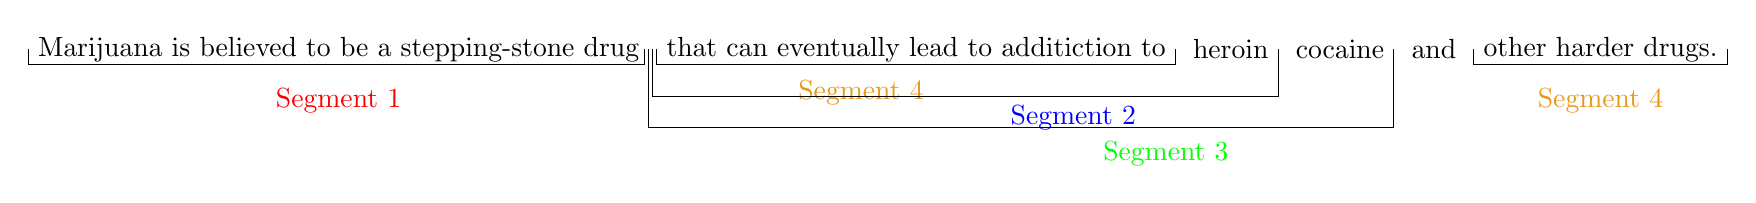
\begin{tikzpicture}[node distance=1mm]
\node (s1) {Marijuana is believed to be a stepping-stone drug};
\node (s234) [right=of s1]{that can eventually lead to additiction to};
\node (s2) [right=of s234]{heroin};
\node (s3) [right=of s2]{cocaine};
\node (o) [right=of s3] {and};
\node (s4) [right=of o] {other harder drugs.};

\node (s1lab) [below=of s1] {\textcolor{red}{Segment 1}};
\node (s2lab) [below=of s2, xshift=-2cm, yshift=-2.5mm] {\textcolor{blue}{Segment 2}};
\node (s3lab) [below left=1cm of s3, xshift=1mm, yshift=-1mm] {\textcolor{green}{Segment 3}};
\node (s4lab1) [below=of s234, xshift=-0.7cm, yshift=1mm] {\textcolor{orangegreen}{Segment 4}};
\node (s4lab2) [below=of s4] {\textcolor{orangegreen}{Segment 4}};
\draw [-]
($(s1.east) - (0.5mm, 0)$)
-- ++(0, -.2)
-| ($(s1.west) $);

% S4 segment
\draw [-]
($(s234.east) $)
-- ++(0, -0.2)
-| ($(s234.west) - (0, 0) $);

% S2 segment
\draw [-]
($(s234.west) - (0.5mm, 0)$)
-- ++(0, -0.6)
-| ($(s2.east) $);

% S3 segment
\draw [-]
($(s234.west) - (1mm, 0)$)
-- ++(0, -1.0)
-| ($(s3.east) $);

% other S4 segment
\draw [-]
($(s4.west) $)
-- ++(0, -.2)
-| ($(s4.east) $);
\end{tikzpicture}
	\caption{An example of post made in the ``Marijuana'' topic. 
	\textcolor{red}{Segment 1} is a regular segment. 
	\textcolor{blue}{Segment 2} and \textcolor{green}{Segment 3} are mutually overlapping.
	\textcolor{orangegreen}{Segment 4} is both overlapping and discontiguous.}
	\label{fig:segment_example_range}
\end{figure}

%'<S1>Marijuana is believed to be a stepping-stone drug
%</S1><S2><S3><S4>that can eventually lead to addiction to
%</S3></S4>heroin,</S2><S3> cocaine</S3> and<S4> other harder
%drugs.</S4>'

% <S1>Nothing can bring peace to this earth.</S1> <S2>Its a great idea to try and
% push for world peace</S2> <S3>but it will never happen...</S3>'


\section{Discussion and Conclusion}


%\chapter{Claim Microstructures}

%This chapter describes claim microstructures


% microstructure vs. ontologies
\chapter{Formalizing claims}
\label{chap:formalization}

In the previous chapter we have explored how to identify claims in text. 
Now, we wish to lay the ground work for the next step: structuring those claims. 
To do so, we first need a model according to which the claims will be structured. 
Unlike most approaches in argumentation mining and computational argumentation that
assume a claim is atomic, we wish to work on the sub-claim level in an attempt to 
derive a logical representation of claims. 

% TODO this needs further writing
This chapter is divided into two main parts.  In the first part, the
microstructure formalism is introduced (section~\ref{sec:for_microstructures}).
In the second part (section~\ref{sec:ontology_formalization}), we introduce a a
formalization based on ontologies. To demonstrate examples of both formalization
standards, we first take the dataset of claims and their respective paraphrases
described in section~\ref{sec:claim_seg_data}. We then formalize claims 
according to the microstructure and ontology standard.
Finally, we conclude in section~\ref{sec:formalization_conclusion}.

\section{Microstructures}
\label{sec:for_microstructures}

\begin{figure}
	\begin{center}
      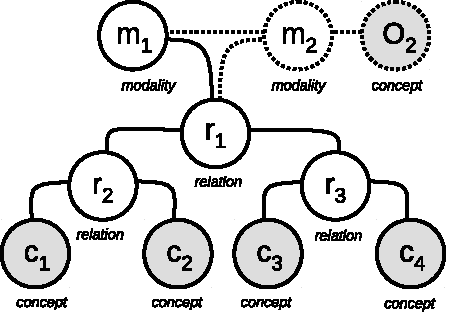
\includegraphics[scale=1]{microstructure.pdf}
      \end{center}
      \caption{Claim microstructure (2nd-order).}
  \label{fig:structures_flowchart}
\end{figure}

Microstructures are structures expressing relations between the domain-specific
concepts, reflecting beliefs, value judgements, or desired policies of the claim
author. Their purpose is to capture the gist of the claim. 
They stemmed from as many claims could be expressed as a \emph{relation}
between \emph{concepts} using a certain \emph{modality}. 
Figure~\ref{fig:structures_flowchart} shows a claim microstructure bringing three elements 
together. 

\paragraph{Relations. }  Many claims can be represented as expressing a
relation between two concepts. For example, on the topic of ``Gay Rights'', 
the relations may be `\texttt{promotes(gay marriage, depopulation)}' and 
`\texttt{purpose(love, procreation)}'. 
There are also comparably fewer claims that can be expressed via
higher-order relations , e.g. `\texttt{entails(constitution, allow(state, gay marriage))}. 
Each relation can be negated, e.g. $\neg$\texttt{promotes(gay marriage,
depopulation)} expresses that gay marriage does not cause depopulation. 
Relations are domain independent. 

\paragraph{Concepts. }
The relations are established between concepts, expressed by noun phrases. 
For ease of access, they can be arranged into a small, domain specific taxonomy of concepts. 
For instance ``gay marriage'', ``heterosexual marriage'' and ``religious marriage''
all belong under the concept of ``marrriage''. 
The taxonomic relations could also be useful for later computational processing. 
Concepts are domain dependent and need to defined for each topic anew

\paragraph{Modalities. }
We observe that claims are expressed under different modalities. 
They can be roughly categorized into \textit{beliefs, value judgements, and policies}. 
We formalize this via unary relations `believes', `approves', `disapproves',
and `desires' corresponding 
to beliefs (factual, religous, and opinion-based), positive value judgements, negative value 
judgements, and desired policy (desired state of affairs) respectively. 
The three modalities act as a wrapper on the propositional content of the claim, 
effectively modulating what is being claimed. 
For instance, `\texttt{believes(purpose(love, procreation))}' expresses the belief 
that love serves procreation, while \texttt{desires(}$\neg$\texttt{allow(state, gay marriage))}'
expresses the wish for the state not to allow gay marriages. 

\paragraph{Second opinion holder. }
Finally, in a number of claims the claim is expressed with a reference to a second
opinion holder (e.g. the Bible, the state). 
To tackle this, we add an additional modality layer with the opinion holder as
an additional modifier. 
For instance `\texttt{believes(believes[state](promotes(marriage, advancement)))}' corresponds
to the belief that the state believes gay marriages lead to an advancement. 
By convention, the opinion holder of the first modality is always the author of the post. 

\begin{table}
{\footnotesize
\begin{tabular}{lp{0.80\columnwidth}}
\toprule
\textbf{Relation} & \textbf{Definition} \\
\midrule
\texttt{promotes(A, B)} & Promoting agent A promotes, fosters, leads, increases likelihood, boosts B.  \\
\texttt{suppress(A, B)} & Suppressing agent A suppresses, decreases likelihood, puts down, vanquishes B \\
\midrule
\texttt{allow(A, B)} & Principle A allows, approves, licenses state of affairs B \\
\midrule
\texttt{entails(A, B)} & State of affairs A, necessarily, per definition or causally, makes B true. \\
\texttt{contradicts(A, B)} & State of affairs A, necessarily, per definition or causally, makes B false. \\
\midrule
\texttt{purpose(A, B)} & The purpose of A is B. \\
\midrule
\texttt{equal(A, B)} & State of affairs A is equal to state of affairs B. \\
\midrule
\texttt{has(A, B)} & A has the properties affected by the existence of B.  \\
\bottomrule
\end{tabular}}
\caption{Relation types in claim microstructures.}
\label{tab:microstructures_relations}
\end{table}

\paragraph{Microstructure formalization. }$\mathcal{R}, \mathcal{C}$, and
$\mathcal{M}$ denote the set of relations, concepts and
modalities, respectively. 
Formally, we define a claim microstructure as a quadruple 
$$
(m_1, m_2, o_2, r)
$$ 
where $m_1 \in \mathcal{M}$, $m_2 \in \mathcal{M} \cup \{\epsilon\}$,
$o_2 \in \mathcal{C} \cup \{\epsilon\}$ is the optional second opinion holder, and 
$r = (t, c_1, c_2) \in \mathcal{R}$ is the (possibly higher order) relation 
between two concepts or relations $c_1, c_2 \in \mathcal{C} \cup \mathcal{R}$
conveyed by the relation type $t$.
Table~\ref{tab:microstructures_relations} lists all possible relation types. 
In chapter~\ref{chap:analysis} we will show
how this microstructure formalization can be used. 
Now that we have formally defined microstructures, we move on to another
formal claim representation. 

\paragraph{Data annotation. }
We use the dataset defined in chapter~\ref{chap:claim_segmentation}
and single out the ``\emph{Gay Rights}'' topic. We end with 100 
posts (50 \pro{pro} and 50 \con{con}) which break down into 920 claims and their
respective paraphrases. We ask two annotators (A1 and A2) to translate each of 
the 920 claims into claim microstructures. The annotators were provided 
with a domain-specific taxonomy on ``\emph{Gay Rights}'', compiled 
based on a manual analysis of claims. The taxonomy consists of 150 concepts
arranged into a tree of maximum depth of four. The annotators
were instructed to use the existing concepts from the taxonomy, and
introduce new ones only if they could not find a suitable one in the
taxonomy. They were also instructed not to use microstructures of order higher 
than two. Full annotation guidelines are listed in
appendix~\ref{sec:microstructure_annotation_appendix}.
Out of 920 claims, annotator A1 managed to translate 882 claims into 707
distinct microstructures while annotator A2 translated 842 claims into
767 distinct microstructures. The average annotation effort was 33 hours. 
The number of claims for which both provided an identical microstructure is only
58 (6.3\%). The annotators introduced 157 new concepts, indicating that the initial 
taxonomy was of too limited a scope. The low annotator agreement and relatively 
large number of added concepts suggest that a fair amount of ambiguity exists
in translating claims to microstructures. Our analysis revealed that, in the majority
of cases, the ambiguity is genuine and in such cases having more candidate 
microstructures for a single claim can be considered advantageous. 
The analysis also revealed that 'believes' is the most frequent modality, used for
79\% of the claims. For A1, \emph{entails} is the most common relation (61\%), while
A2 made a more balanced use of relations, with the top two being \emph{has} (21\%)
and \emph{entails} (15\%). The concepts most frequently used by A1 were
\emph{homosexuality}, \emph{homosexual people}, and \emph{marriage}, while for A2
these are \emph{the Bible}, \emph{homosexual people}, and \emph{government interest}. 

\section{Ontology-based formalization}
\label{sec:ontology_formalization}

Microstuctures provide a claim structure which can then be used 
to ``compress'' the claim for subsequent argumentation tasks
(see application to stance classification in section~\ref{sec:stance_micro}).
However, microstructures do not inherently support any
well-established computer science standard. 
Hence, we turn to ontologies. Using ontologies not only allows for 
formalizing a claim, but also provides inference opportunities within
a well-established frameworks (such as the resource description framework RDF). 

We propose an ontology-based framework ClaimOntology to  formalize claims. The
ontology is key part of a formalization framework which defines how to
bootstrap a claim formalization from scratch. The end product of the workflow
is a ontology containing formalized claims in a specific domain. 
The ontology itself is built on two levels: 
\begin{enumerate*}[label=(\arabic*)]
\item the upper and 
\item the domain ontology 
(the motivation of using two-level ontologies is described in
		section~\ref{sec:knowledge_representation}). 
\end{enumerate*}
The upper ontology formalizes abstract patterns in argumentative
claims as object properties. The domain-level ontology conceptualizes 
a specific discussion domain. The relationship between the upper 
and domain ontology is similar to a predicate-argument
relationship \citep{hindle1990noun}, where the upper ontology
defines argumentation-specific predicates --- defined through object properties, 
and the domain ontology defines arguments --- defined through 
individuals. 

The steps to be able to perform domain-specific claim analysis
involve
\begin{enumerate*}[label=(\arabic*)]
\item domain experts designing the domain ontology,
\item integrating the proposed domain ontology with the upper ontology,
\item defining the claims as individuals in the two-level ontology, and
\item validating claim individuals to ensure quality of fit for
	individuals in the domain ontology
\end{enumerate*}
Completing these steps allows users of the formalization framework
to do deep domain claim analysis for the domain of interest. 
An example of a deep domain analysis is in chapter~\ref{chap:analysis}.

Apart from modeling domain concepts and the relationships amongst them, we also
wish to formalize the \emph{modality} of how the claim was expressed: as facts,
policies, and positive or negative value statements (see definition in
\citep{rieke1997argumentation} and microstructure
section~\ref{sec:for_microstructures}). 

\subsection{ClaimOntology}
\label{subsec:claimontology}

\begin{figure}
	\centering
	\footnotesize
	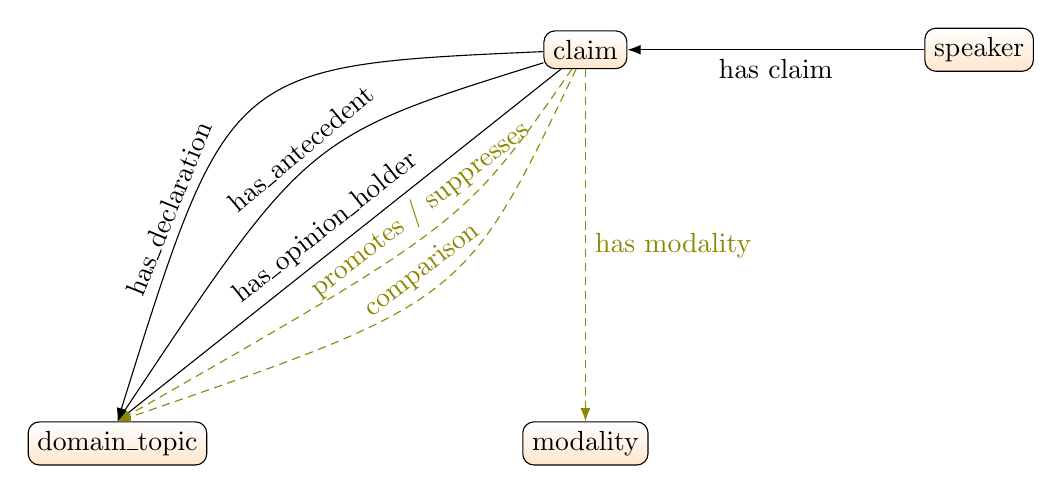
\begin{tikzpicture}[
concept/.style={shape=rectangle, rounded corners,
draw, align=center,
top color=white, bottom color=orange!20},
node distance=5cm,
]
\node[concept] (claim) {claim};
\node[concept, below of=claim] (modality) {modality};
\node[concept, right of=claim] (speaker) {speaker};
\node[concept, left=4cm  of modality] (domain) {domain\_topic};

\draw[-Latex] (speaker) -- (claim) 
	node [midway, below] {has claim}; 

\draw[-Latex, densely dashed, color=olive] (claim) -- (modality)
	node [midway, right] {has modality}; 

\draw [-Latex] (claim) .. controls ($(claim.west) + (-4cm,
-0.2cm)$) ..  ($(domain.north)$) node [sloped, above, near end] {has\_declaration}; 

\draw [-Latex] (claim) .. controls ($(claim.west) + (-3cm,
-1.1cm)$) ..  ($(domain.north)$) node [sloped, above, midway] {has\_antecedent}; 

\draw [-Latex] (claim) --  ($(domain.north)$) node [above, sloped, midway] {has\_opinion\_holder}; 

\draw [-Latex, densely dashed, color=olive] (claim) .. controls ($(claim.west) + (-1cm,
-2.2cm)$) ..  ($(domain.north)$) node [sloped, above, midway] {promotes / suppresses}; 

\draw [-Latex, densely dashed, color=olive] (claim) .. controls ($(claim.west) + (-1cm,
-3.2cm)$) ..  ($(domain.north)$) node [sloped, above, midway] {comparison}; 

\end{tikzpicture}
\caption{Main classes and properties of ClaimOntology. Dashed lines indicate
	semantic properties, full lines structural properties. 
	indicate. Arrow orientation indicates the
	triplet ordering. }
\label{fig:claimontology}
\end{figure}


The upper ontology represents general argumentation patterns, mostly on the claim level. 
The concepts and relations are used across different domains. 
The central object of the upper ontology is the claim class.
We are interested in extracting as much as possible claims from a single topic. 
We leave the levels above the claim (argument) for future work. The proposed
ontology is an OWL second-order description logic (2DL) ontology built using the
Prot\'{e}g\'{e} software \citep{gennari2003evolution}. The four main concepts of the
upper ontology are:
\begin{itemize}
	\item \texttt{claim}, corresponding to any argumentative statement,
	\item \texttt{speaker},  denoting the author of the claim
		(one speaker may be associated with $N$ \texttt{claims})
	\item \texttt{modality}, which is one of fact, value, or policy, and
	\item \texttt{domain\_topic}, representing any individual from the domain ontology.
\end{itemize}

The main concepts are related to each other through different types of object
properties, suitable to represent both the \emph{structural and semantic aspects} of
claims. The former aim at formalizing the structure of claims used in
the argumentation, such as the presence of an antecedent element. The latter
are used to describe the semantic relations in claims, for instance that
an element causes another one. Thus, on one hand, the attempt of 
formalizing structural aspects improves the analysis of structuring and
forming process of argumentation. On the other hand, this type of formalization
is allows for a semantic analysis of building blocks, namely claims, used in 
argumentative discussions. Among the \emph{structural properties}, we identify:
\begin{itemize}
\item \texttt{has\_declaration}, 
\item \texttt{has\_antecedent},
\item \texttt{has\_opinion\_holder}, and
\item \texttt{has\_claim}. 
\end{itemize}
The \texttt{has\_declaration} property indicates an acknowledgement of
existence of a domain individual. For example, the claim 
\emph{marijuana consumption is out there} acknowledges
the existence of the domain individual \emph{marijuana consumption}.
The \text{has\_antecedent} property indicates the presence of an 
antecedent in a claim. The antecedent is always paired with some
form of a consequent, which is a semantic property. To indicate
there is a second opinion holder the \texttt{has\_opinion\_holder}
property is used. The role of the \texttt{has\_opinion\_holder}
property is equivalent to the second opinion holder in the microstructure
formalization (see section~\ref{sec:for_microstructures}). Finally, the speaker
who made the claim is attributed using the \texttt{has\_claim} property.

We discern between three different types of \emph{semantic properties}:
\begin{itemize}
\item \texttt{promotes / suppresses},
\item \texttt{comparison}, and
\item \texttt{has\_modality}
\end{itemize}
The \texttt{promotes / suppresses} property is used to represent the claim
consequent as either a \texttt{promotes} or \texttt{suppresses} property
(inspired by \citet{hashimoto2012excitatory}). It is always paired with
the \texttt{has\_antecedent} structural property. The \texttt{promotes}
property has subproperties with \texttt{causes} and \texttt{implies}
properties, whereas the \texttt{suppresses} property has 
subproperties \texttt{implies} and \texttt{does\_not\_cause}.
The claim \texttt{claim\_x} made by \texttt{speaker\_x}
\emph{smoking marijuana hurts your lungs} can then be formalized as triplets:
\begin{align*}
	< & \mathit{claim\_x}, \hspace{0.1cm} \mathit{has\_antecedent}, \hspace{0.1cm}
	\mathit{marijuana\_consumption} > \\
	< & \mathit{claim\_x}, \hspace{0.1cm} \mathit{suppresses}, \hspace{0.1cm}
	\mathit{lung\_health} > 
\end{align*}
Alternatively, it may also be formalized in a negation fashion as:
\begin{align*}
	< & \mathit{claim\_x}, \hspace{0.1cm} \mathit{has\_antecedent}, \hspace{0.1cm}
	\mathit{marijuana\_consumption} > \\
	< & \mathit{claim\_x}, \hspace{0.1cm} \mathit{causes}, \hspace{0.1cm}
	\mathit{lung\_damage} > 
\end{align*}
The \texttt{comparison} property is used to formalize a comparison of 
two domain concepts. There are three comparison object properties (each with the
\texttt{domain\_topic} as the object individual): \texttt{comparison\_greater},
\texttt{comparison\_less}, and \texttt{comparison\_criterion}. The
\texttt{comparison\_criterion} is optional and is used to denote the feature of 
comparison. For example, the claim \emph{alcohol is worse for your health than marijuana} can
be formalized as:
\begin{align*}
	< & \mathit{claim\_x}, \hspace{0.1cm} \mathit{comparison\_greater}, \hspace{0.1cm}
	\mathit{alcohol} > \\
	< & \mathit{claim\_x}, \hspace{0.1cm} \mathit{comparison\_less}, \hspace{0.1cm}
	\mathit{marijuana} >  \\
	< & \mathit{claim\_x}, \hspace{0.1cm} \mathit{comparison\_property}, \hspace{0.1cm}
	\mathit{health} > 
\end{align*}
The \texttt{has\_modality} property reflects in which modality the claim was made. 
Claims \emph{marijuana should be legalized} and \emph{marijuana is legalized} 
can be formalized to have different modalities for the same domain concepts
(\emph{marijuana\_legalization}). 

The main classes and properties of ClaimOntology are visualized in 
figure~\ref{fig:claimontology}. The domain ontology defines 
claim individuals as claims made by speakers of the
\texttt{domain\_individual} type. Thus, the domain individuals need to be
defined before making claim individuals. Now, we show a full formalization 
example on \emph{claim\_x} which states
\emph{heavy industry did not cause climate change}. Here, we may establish
two domain individuals: \texttt{industry} and \texttt{climate change}
connected via a \texttt{cause} property. Note that we omit the \emph{industry}
adjective \emph{heavy} which is a decision left to the domain expert to decide
on the granularity level of the domain ontology. 
More formally, we define \texttt{claim\_x} to contain properties:
\begin{align*}
	< & \mathit{claim\_x}, \hspace{0.1cm} \mathit{has\_antecedent}, \hspace{0.1cm}
	\mathit{industry} > \\
	< & \mathit{claim\_x}, \hspace{0.1cm} \mathit{does\_not\_cause}, \hspace{0.1cm}
	\mathit{climate\_change} >  \\
	< & \mathit{claim\_x}, \hspace{0.1cm} \mathit{has\_modality}, \hspace{0.1cm}
	\mathit{fact} > 
\end{align*}

We define claims as done in section~\ref{sec:claim_seg_data}, also 
abiding by nine principles. We reuse the claims and their paraphrases 
annotated in section~\ref{sec:claim_seg_data} to formalize in ClaimOntology. 

\begin{algorithm}[t]
	\footnotesize{
	\begin{algorithmic}[1]
%\begin{Verbatim}[commandchars=\\\{\},codes={\catcode`$=3\catcode`_=8}]

\Function{viewpoint}{claim}
\State \begin{varwidth}[t]{\linewidth}
      map~$\gets$~"policy": "It should be that ", \par
        \hskip\algorithmicindent "good\_value": "I approve that ", \par
        \hskip\algorithmicindent "bad\_value": "I approve that ", \par
        \hskip\algorithmicindent "fact": ""
      \end{varwidth}

	\State 
	\Return map[claim.viewpoint]
\EndFunction
\State

\Function{negate}{claim, object}
\If{claim is\_negated}
\State
\Return " does not " + object
\Else
\State
\Return object
\EndIf

\EndFunction
\State

\If{claim.nary == 1}
	\State object $\gets$ claim.property["has\_declaration"].object
	\State
	\Return viewpoint(claim) + negate(claim, object) + "exist"
\EndIf
\State
\If{claim.nary == 2}
	\State ante $\gets$ claim.property["has\_antecedent"].object
	\State cons $\gets$ claim.property["promotes"].object
	\State
	\Return viewpoint(claim) + ante + negate(claim, object) + cons
\EndIf
\State
\If{claim.nary = 3}
	\State less $\gets$ claim.property["comparison\_less"].object
	\State more $\gets$ claim.property["comparison\_greater"].object
	\State prop $\gets$ claim.property["comparison\_property"].object
	\State

	\State exp $\gets$ more + " is greater than " + less + " by " + prop
	\Return viewpoint(claim) + exp
\EndIf
\end{algorithmic}



% \textbf{function} viewpoint (claim)
%  map $\gets$ "policy": "It should be that ",
%         "good\_value": "I approve that ",
%         "bad\_value": "I disapprove that "
%         "fact": "
% \textbf{return} map[claim.viewpoint]
% 
% \textbf{function} negate (claim, object)
%   \textbf{if} claim is\_negated
%     \textbf{return} " does not " + object
%   \textbf{else} 
%     \textbf{return} object
%   \textbf{end if}
% 
% \textbf{if} claim.nary == 1
%   object = claim.property["has\_declaration"].object
%   \textbf{return} viewpoint(claim) + negate(claim, object) + "exist"
% 
% \textbf{if} claim.nary == 22
%   ante = claim.property["has\_antecedent"].object
%   cons = claim.property["promotes"].object
%   \textbf{return} viewpoint(claim) + ante + negate(claim, object) + cons
% 
% \textbf{if} claim.nary == 3
%   less = claim.property["comparison\_less"].object
%   more = claim.property["comparison\_greater"].object
%   prop = claim.property["comparison\_property"].object
% 
%   exp $\gets$ more + " is greater than " + less + " by " + prop
%   \textbf{return} viewpoint(claim) + exp
% \end{Verbatim}
}
\caption{Algorithm to generate a natural language sentence from a formalized
	claim individual}
\label{alg:formalization_to_sentence}
\end{algorithm}

To validate how well the formalized claims represent the original claims
made by the speakers, we propose measuring textual entailment between the formalized 
and the original claim. Textual Entailment (\textbf{TE}) models take a pair 
of sentences and predict whether the facts in the first sentence necessarily imply
facts in the second sentence (see section~\ref{sec:textual_entailment} for a
a short introduction to textual entaiment). Textual entailment expects 
sentences, so we have to translate the formalized claim back to natural language. 
For that purpose, we build algorithm~\ref{alg:formalization_to_sentence} which 
very roughly produces natural language sentences from formalizations. 
We acknowledge that produced sentences may not always be grammatical (depending on the
domain ontology). Using algorithm~\ref{alg:formalization_to_sentence} on the claim 
\texttt{claim\_y} with properties:
\begin{align*}
	< & \mathit{claim\_y}, \hspace{0.1cm} \mathit{comparison\_greater}, \hspace{0.1cm}
	\mathit{alcohol} > \\
	< & \mathit{claim\_y}, \hspace{0.1cm} \mathit{comparison\_less}, \hspace{0.1cm}
	\mathit{marijuana} >  \\
	< & \mathit{claim\_y}, \hspace{0.1cm} \mathit{comparison\_property}, \hspace{0.1cm}
	\mathit{mind\_influental} >  \\
	< & \mathit{claim\_y}, \hspace{0.1cm} \mathit{has\_modality}, \hspace{0.1cm}
	\mathit{fact} > 
\end{align*}
produces the sentence \emph{alcohol is more than marijuana by being mind influental}.
Now, we compare this claim to the original and paraphrased claim via 
textual entailment models. Textual entailment estimates how well 
formalized claims represent original claims. To calculate
textual entailment between the (original or paraphrased) claim and reconstructed
formalized claim, we use the decomposable attention model \citep{parikh2016decomposable}
(available via Allennlp \citep{gardner2018allennlp}) which performs
close to the state-of-the-art on the widely used SNLI dataset \citep{bowman2015large}.

\subsection{Use-case: ``Marijuana'' }
\label{sec:usecase_ontology}

\begin{figure}
	\centering
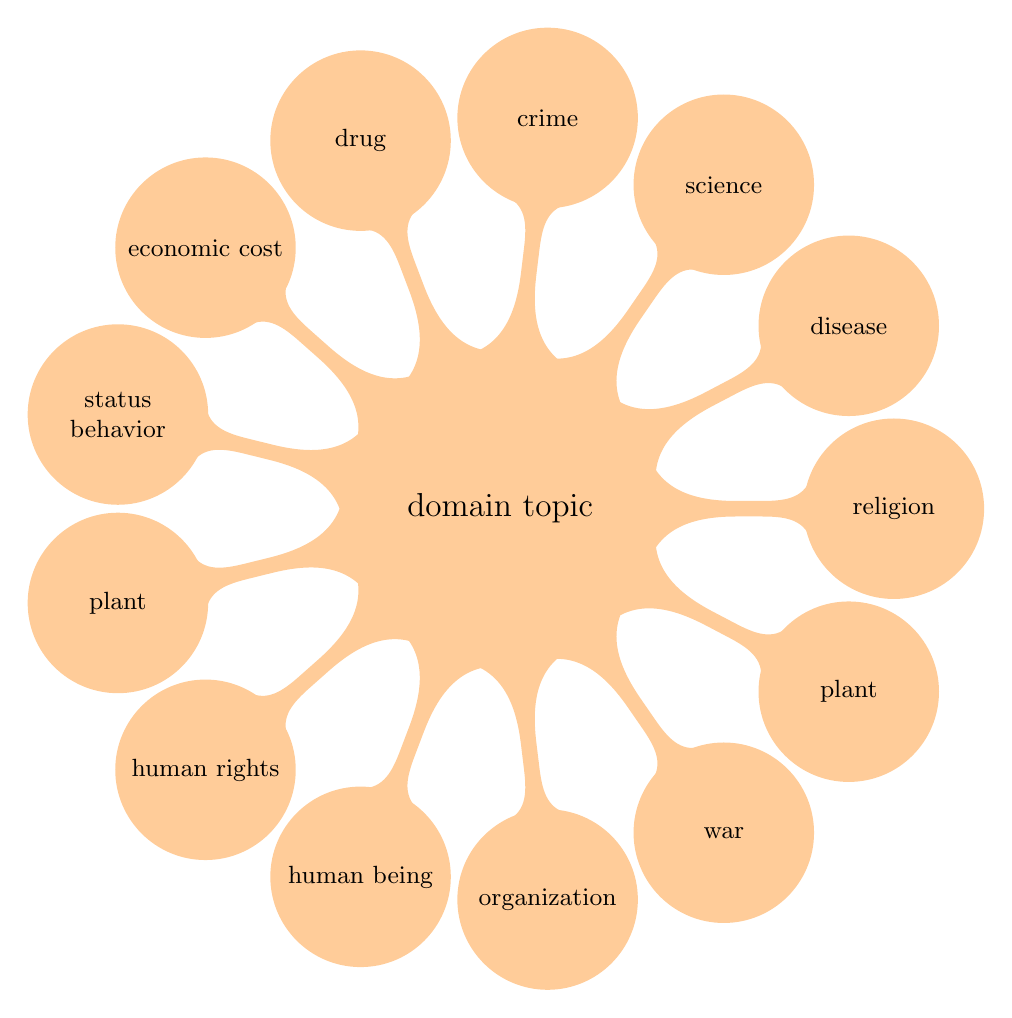
\begin{tikzpicture}
\path [mindmap, grow cyclic, level 1/.append style={sibling angle=360/13},
concept color=orange!40,
]
node [concept] {domain topic}[clockwise from=0]
	child { node[concept] {religion}}
	child { node [concept]{plant}}
	child { node[concept] {war}}
	child { node[concept] {organization}}
	child { node[concept] {human being}}
	child { node[concept]  {human rights}}
  child {  node[concept] {plant}}
  child {  node[concept] {status behavior}}
  child {  node[concept] {economic cost}}
  child {  node[concept] {drug}}
  child {  node[concept] {crime}}
  child {  node[concept] {science}}
  child {  node[concept] {disease}};
  child {  node[concept] {society effect}};
	
\end{tikzpicture}
\caption{Marijuana legalization domain ontology classes}
\label{fig:marijuana_domain_ontology}
\end{figure}


Now, we wish to apply the ClaimOntology to the ``\emph{Marijuana}'' topic in
two steps.  First, we construct a domain ontology ``\emph{Marijuana
legalization}''.  Second, we formalize claims from the ``\emph{Marijuana}''
topic as claim individuals. 

The domain ontology should contain domain specific classes, properties, and
instances. The idea is to build the domain ontology in a data driven 
fashion from speakers' claims. We build the domain ontology in two steps:
\begin{enumerate*}[label=(\arabic*)]
\item building the domain ontology of concepts, and 
\item claim individual annotation. 
\end{enumerate*}
After completing those two steps, the ontology can be used in a claim analysis. 

A domain ontology conceptualizes the specific domain of the online discussion. 
It is usually recommended to have some central terms around which to build
around (i.e. \emph{person}). We inspect claims in the ``\emph{Marijuana}'' topic,
using noun phrases as likely candidates for classes. We introduce
data properties mainly for noun phrases with some varying nuance relevant to
the domain. One example of using a data property would be to disambiguate between
\emph{illegal abortion} and \emph{legal abortion} by using boolean data
property \emph{legal} with the concept of \emph{abortion}.
Individuals of the domain ontologies should reflect all realizations of a concepts as
it appears in text. So, if we have a concept of \emph{taxes}, we require a concept
that covers all linguistic realizations in text, such as \emph{government tribute} or
\emph{compulsory state fee}. 

\begin{figure}
	\centering
	\footnotesize
	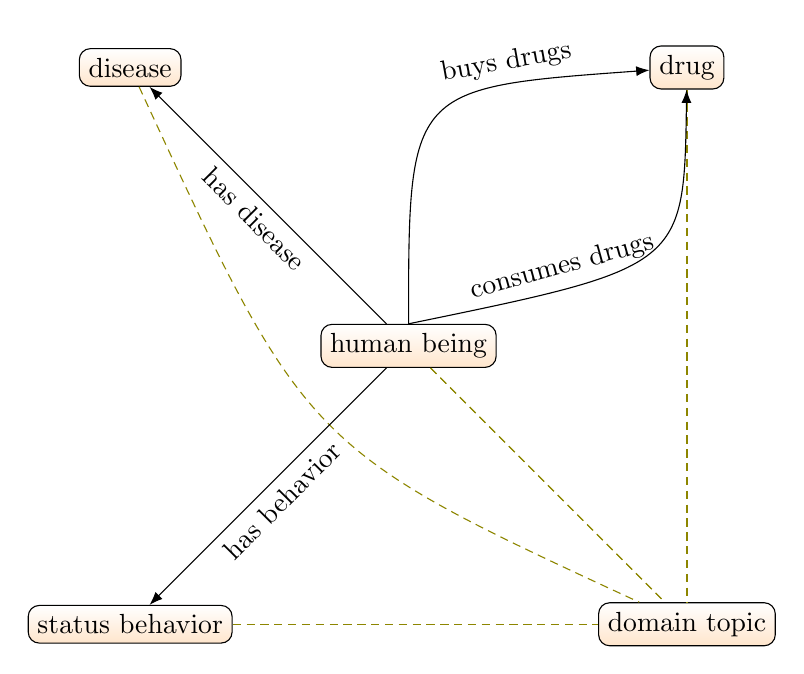
\begin{tikzpicture}[
concept/.style={shape=rectangle, rounded corners,
draw, align=center,
top color=white, bottom color=orange!20},
node distance=5cm,
]
\node [concept] (human) {human being};
\node [concept, below right of=human] (domain) {domain topic};
\node [concept, above left of=human] (disease) {disease};
\node [concept, below left of=human] (status) {status behavior};
\node [concept, above right of=human] (drug) {drug};

\draw[densely dashed, color=olive] (human) -- (domain);
\draw[densely dashed, color=olive] (disease) .. controls ($(human) + (-1.3cm,
		-1.3cm)$) .. (domain); 
\draw[densely dashed, color=olive] (status) -- (domain); 
\draw[densely dashed, color=olive] (drug) -- (domain); 
\draw[densely dashed, color=olive] (human) -- (domain); 

\draw [-Latex] (human.north) .. controls ($(human.north) + (0cm,
3cm)$) ..  (drug) node [sloped, above, near end] {buys drugs}; 
\draw [-Latex] (human.north) .. controls ($(human) + (3.5cm, 1cm)$)
..  (drug) node [sloped, above, near start] {consumes drugs}; 
\draw [-Latex] (human) -- (status) node [below, midway, sloped] {has behavior}; 
\draw [-Latex] (human) -- (disease) node [below, midway, sloped] {has disease}; 

\end{tikzpicture}
\caption{Main classes and properties of the \textit{marijuana} domain 
ontology. 
Dashed lines indicate subclasses, full lines indicate object properties. 
The triple (\texttt{human\_being}, \texttt{buys\_drugs}, \texttt{drug}) represents an 
individual that belongs to the
\texttt{human\_being} class, which posses the property \texttt{buys\_drugs} with 
object \texttt{drug}.
} 
\label{fig:main-classes}
\end{figure}

The ``\emph{Marijuana legalization}'' domain ontology is built by experts over
several iterations with reviews in-between rounds. The end result proposes 
\texttt{domain\_topic} concepts, properties, and individuals. The resulted
domain ontology produced a diverse set of concepts, such as states (\texttt{war}),
people (\texttt{drug\_consumer}), or general abstract events (\texttt{society\_effect}). 
The top level classes of the ontology are displayed in 
Fig.~\ref{fig:marijuana_domain_ontology}. The relationships between some of the more frequently
used classes are shown in Fig.~\ref{fig:main-classes}. 
Individuals instantiate classes
and use properties. In total, 75 domain individuals were created, some of those
being \texttt{marijuana addicted consumer}, \texttt{legalized marijuana}, \texttt{
legalized alcohol}, \texttt{reduced mental capability}, etc. 
Fig.~\ref{fig:drug_domain_individuals} shows the hierarchy classes and 
individuals stemming from the drug class. 

\begin{figure}
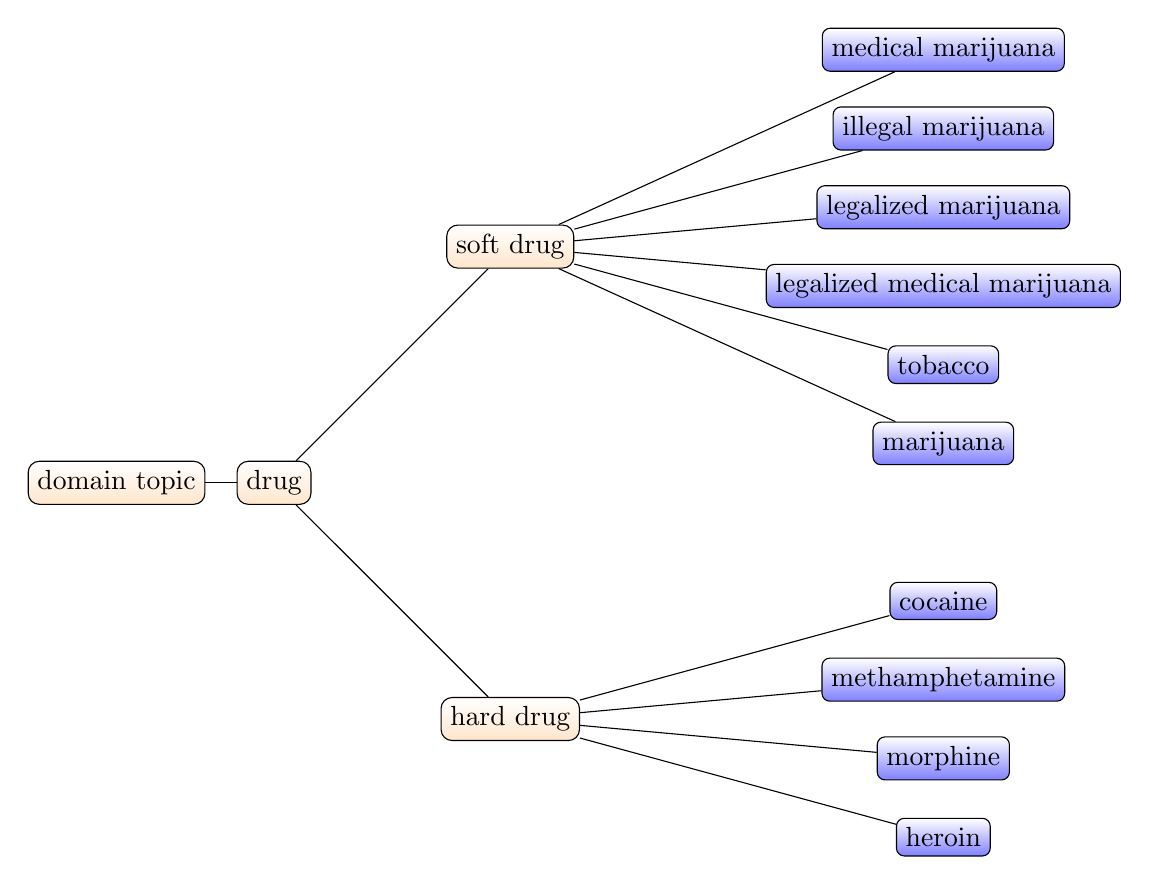
\begin{tikzpicture}
[grow'=right,
level 1/.style={sibling distance=1.5cm, level distance=2cm},
level 2/.style={sibling distance=1.5cm, level distance=3cm, },
level 3/.style={
sibling distance=1cm, level distance=5.5cm},
concept/.style=
{shape=rectangle, rounded corners,
draw, align=center,
top color=white, bottom color=orange!20},
individual/.style={rectangle, rounded corners=1mm, draw, top color=white, bottom color=blue!50,
text centered}
	]
	\node (root) [concept] {domain topic}
	child  { node [concept] {drug}
	child  { node [concept] {soft drug} 
	child { node [individual] {medical marijuana}}
	child { node [individual] {illegal marijuana}}
	child { node [individual] {legalized marijuana}}
	child { node [individual] {legalized  medical marijuana}}
	child { node [individual] {tobacco}}
	child { node [individual] {marijuana}}
    }
    child [missing]
    child [missing]
    child [missing]
    child {node  [concept]{hard drug}
	child {node [individual] {cocaine}}
	child {node [individual] {methamphetamine}}
	child {node [individual] {morphine}}
	child {node [individual] {heroin}}
    }
};
	
\end{tikzpicture}
\caption{Marijuana legalization domain ontology drug individuals. 
	Classes/entities and orange and individuals are blue. }
	\label{fig:drug_domain_individuals}
\end{figure}

\begin{table*}[t]
	\begin{tabular}{p{5cm}|p{5cm}|p{5cm}}
	\toprule
Original & Paraphrased & Formalized \\
\midrule
Pot hurts you & Marijuana is bad for your health & Marijuana consumption has negative health effects \\

One may suffer or develop hallucinations, &                                                                                            
When one is under the influence of marijuana, one may hallucinate. &       
marijuana consumer causes mind influential \\ 

Cannabis has been proven to have health benefits . & 
Marijuana has been proven to have health benefits. & 
marijuana suppresses negative health effect \\

legalization would open up a larger market for vaporizers, &                                                                                          
Legalizing marijuana would open up a larger market for vaporizers. &                                           
legalized marijuana promotes free market marijuana seller \\

YOU WILL DIE IF YOU USE THIS TO OFTEN &                                                                     
Using marijuana too often causes death. &                                                                                                                                                     
marijuana consumer promotes death \\                                                         
\bottomrule
\end{tabular}
\label{tab:ontology_annotation}
\caption{Annotation examples. Original represents the unedited speakers' claim.
	Paraphrased represents the from canonical claim made by the annotators.
	Formalized is the text version  of the formalized claim (obtained by
	applying algorithm~\ref{alg:formalization_to_sentence} on a formalized
	claim)
	}
\end{table*}

The ontology with domain individuals can now be merged with the upper ontology. 
Next, we move on to annotating claim individuals. Three expert annotators
formalize 920 claims from the ``\emph{Marijuana}'' topic. A few annotation
example listed in table~\ref{tab:ontology_annotation}.
They fail to formalize 56, 53, and 60 claims, which makes about 6\% of the dataset. 
There are multiple reasons on why a claim is not suitable to be formalized. 
For one, a claim may be lacking appropriate domain individuals, such as in the claim
\emph{tobacco odors dissipate quickly} where we \emph{tobacco odor} is a concept
not seen when building the domain individuals. Other non-formalized claims
deemed to abstract in meaning, an example being \emph{nothing can bring 
world peace}. In 243 out of 920 claims, the same formalization was produced 
by all three annotators, whereas for 325 two out of three annotators agreed. 
Upon manually checking formalizations at random, we observe that some
formalizations were different, yet equally suitable. After annotating and manually
checking claim individuals, we move on to  automatic validation. 

With the domain ontology built and integrated with the upper ontology and claim
individuals annotated, it is considered a good practice to verify and validate
the resulting ontology. 
We first verify the ontology using Prot\'{e}g\'{e} to ensure logical
consistency. For validity, we estimate how much do formalized claims entail 
speakers' original claims by measuring textual entailment between the formalized
and original (or paraphrased) claim. 
Now, we compare formalized sentences to paraphrased claims, excluding 169 claims 
which at least one of the annotators deemed unsuitable to formalize. 
We use an off-the-shelf entailment system which outputs a decision $d \in \{E, C, N\}$
along with normalized decision probabilities, where $E$ stands for entailment, 
$C$ stands for contradiction, and $N$ for neutral (neither an entailment or 
contradiction relation hold). Since entailment is not a symetric relation, we
measure by setting the claim as both the text and hypothesis. 

Measuring entailment across all three anotators, we observe 2591 pairs of claims
and formalizations. The entailment decision was made in 1323 (51\%), 1031 (40\%)
were neutral, whereas contradiction was found in the fewest number of pairs, 
237 (9\%). We compare this a randomized baseline where claims were 
paired with a randomly selected formalized claim. 
We obtain that the entailment decision was made in 
%TODO add numbers for random decisions
We manually inspect some of the examples to determine why were some 
pairs labelled as contradictions or neutral. 
% TODO add examples on false positives
Since the evaluation showed entailment decisions in 
% percent more 
than the randomized baseline, and that the contradiction-labelled examples 
seem to be hard to capture by the entailment system, we feel confident for this ontology
to pass the entailment validation step. 

\section{Conclusion}
\label{sec:formalization_conclusion}

In this chapter, we proposed two formalizations of argumentative claims.  The
first, microstructures define a domain dependent taxonomy of concepts and
define relations amongst concepts. We annotate 920 claims from the ``\emph{Gay
Rights}'' topic. A high number of claims (93\%) was succesfully translated to
microstructures.  However, it showed that two annotators managed to produce the
identical microstructure in only 58 (6.3\%) cases in addition to introducing
157 new concepts. Although some of the differences can be attributed to
microstructure ambiguity, this inter-annotator agreement rate is considered
very low. 
The second proposed formalization is based on ontologies. 
The ontology formalization, ClaimOntology is built from an upper and 
domain ontology. We annotate 920 claims from the ``\emph{Marijuana}''
topic. Similarly to microstructures, a high number (94\%) of the dataset of
successfully formalized.
But, unlike microstructures, inter-annotator agreement was much higher, with 
61\% of claims having at least two identical formalizations. 

Microstructure and ontology formalizations represent first steps
towards sub-claim formalizations. 
Both model the linguistic argumentation patterns
joined with the the domain knowledge. 
Having formalized claims will allow us various applications in 
argumentation mining. In chapter~\ref{chap:analysis}, we will use
microstructures in stance classification, and 
claim ontologies to deriving implicit claims. 
Additionally, in chapter~\ref{chap:claim_structuring} we will explore
how feasible it is to automatically acquire formalized
claims directly from text.  



\chapter{Claim Structuring}

This chapter talks about how claims should be structured \\


\section{Joint model}


\begin{figure}
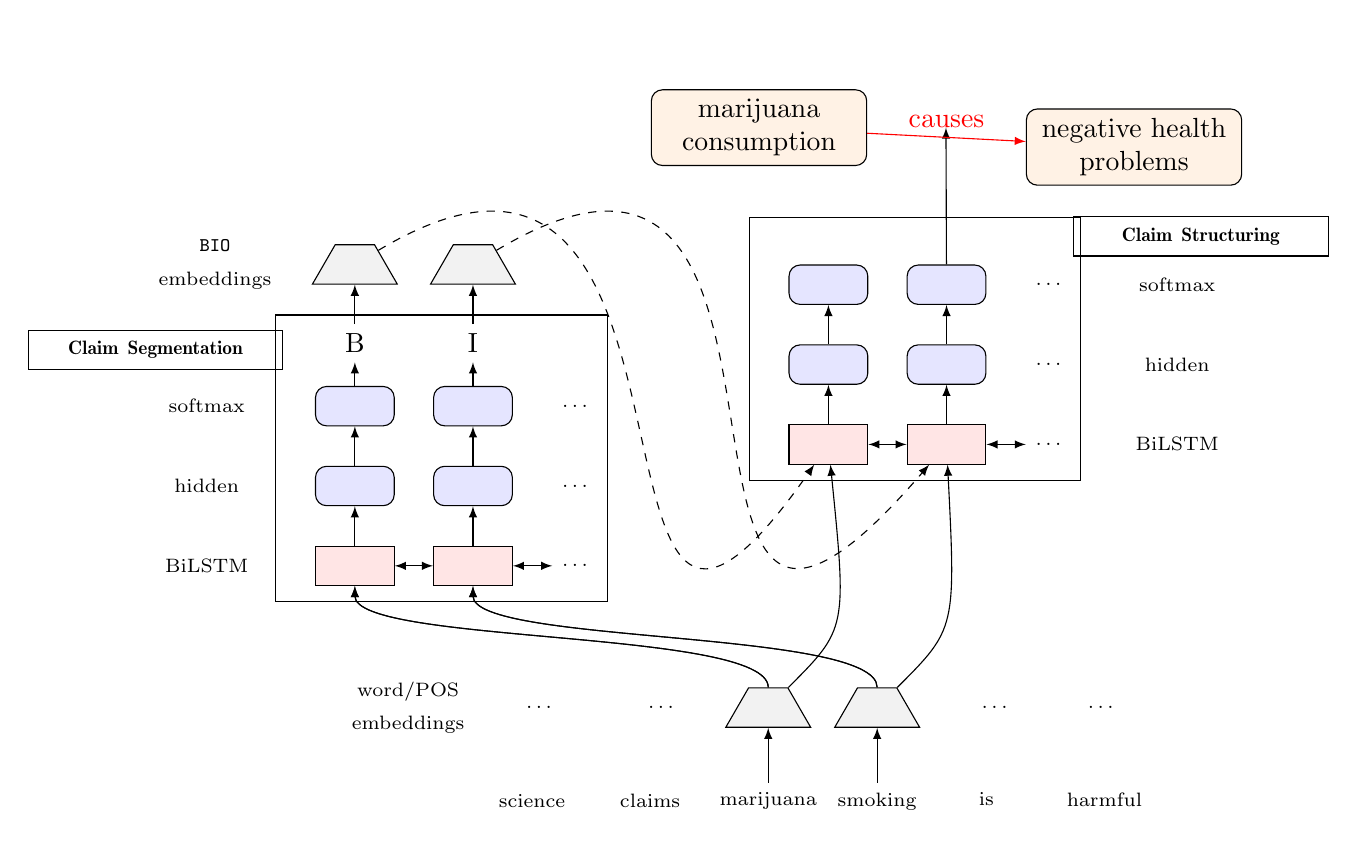
\begin{tikzpicture}[node distance=1.5cm]
\tikzstyle{lstm} = 
[rectangle, minimum width=1cm, minimum height=0.5cm, text
centered, draw=black, fill=red!10]
\tikzstyle{hidden} = 
[rectangle, minimum width=1cm, minimum height=0.5cm, text 
centered, draw=black, fill=blue!10, rounded corners]
\tikzstyle{embed} = 
[trapezium, minimum width=1cm, minimum height=0.5cm, text 
centered, draw=black, fill=gray!10]
\tikzstyle{label} = 
[minimum width=1cm, minimum height=0.5cm, text 
centered, text width=1.5cm]
\tikzstyle{dots} = 
[minimum width=0.3cm, 
minimum height=0.5cm, text 
centered, text width=0.3cm]
\tikzstyle{component} = 
[minimum width=1cm, minimum height=0.5cm, text 
centered, text width=3cm, rectangle, draw=black]
\tikzstyle{concept} =
[rectangle, minimum width=1cm, minimum height=0.5cm, text 
centered, draw=black, fill=orange!10, rounded corners, text width=2.5cm]

\node (lstm_1) [lstm] {};
\node (lstm_2) [lstm, right of=lstm_1] {};
\node (dots_1) [dots, right=0.5cm of lstm_2] {\scriptsize{\dots}};
\node (hidden_1) [hidden, above=0.5cm of lstm_1] {};
\node (hidden_2) [hidden, above=0.5cm of lstm_2] {};
\node (dots_2) [dots, right=0.5cm of hidden_2] {\scriptsize{\dots}};

\node (hidden_3) [hidden, above=0.5cm of hidden_1] {};
\node (hidden_4) [hidden, above=0.5cm of hidden_2] {};
\node (dots_3) [dots, right=0.5cm of hidden_4] {\scriptsize{\dots}};

\node (B_lab) [above=0.3cm of hidden_3] {B};
\node (I_lab) [above=0.3cm of hidden_4] {I};

\node (trapez_1) [embed, above=0.5 cm of B_lab] {};
\node (trapez_2) [embed, above=0.5 cm of I_lab] {};

\draw ($(hidden_3.north west) + (-0.5, 0.9)$) rectangle ($(lstm_2.south east) + (1.2, -0.2)$);

\node (word_1) [below right=2.5cm and 4cm of lstm_1] {\scriptsize{marijuana}};
\node (word_2) [below right=2.5cm and 4cm of lstm_2] {\scriptsize{smoking}};
\node (word_3) [right of=word_2] {\scriptsize{is\textcolor{white}{jg}}};
\node (word_4) [right of=word_3] {\scriptsize{harmful\textcolor{white}{jg}}};
% \node (word_0) [left of=word_1] {\scriptsize{\dots}};
% \node (word_5) [right of=word_4] {\scriptsize{\dots}};
\node (word_m1) [left of=word_1] {\scriptsize{claims}};
\node (word_m2) [left of=word_m1] {\scriptsize{science}};

\node (w_1) [embed, above=0.7cm of word_1] {};
\node (w_2) [embed, above=0.7cm of word_2] {};
\node (dots_word1) [dots, right=0.8cm of w_2] {\scriptsize{\dots}};
\node (dots_word4) [dots, right=0.8cm of dots_word1] {\scriptsize{\dots}};
\node (dots_word2) [dots, left=0.7cm of w_1] {\scriptsize{\dots}};
\node (dots_word3) [dots, left=1cm of dots_word2] {\scriptsize{\dots}};

\node (lstm_3) [lstm, above right=-1 cm and 3.5cm of hidden_4] {};
\node (lstm_4) [lstm, right of=lstm_3] {};
\node (hidden_5) [hidden, above=0.5cm of lstm_3] {};
\node (hidden_6) [hidden, above=0.5cm of lstm_4] {};
\node (hidden_7) [hidden, above=0.5cm of hidden_5] {};
\node (hidden_8) [hidden, above=0.5cm of hidden_6] {};
\node (lstm2_dots_1) [dots, right=0.5cm of lstm_4] {\scriptsize{\dots}};
\node (lstm2_dots_2) [dots, right=0.5cm of hidden_6] {\scriptsize{\dots}};
\node (lstm2_dots_3) [dots, right=0.5cm of hidden_8] {\scriptsize{\dots}};

%\node (struc) [above=0.8cm of hidden_8] {};
\node (c_marijuana) [concept, above left=1.25 cm and 0.5cm of hidden_8] {marijuana consumption };
\node (c_health) [concept, above right=1cm and 0.5cm of hidden_8] {negative health problems};
\draw[-latex] (hidden_8) -- ($(c_marijuana.east) + (1, 0) $);

\draw[-latex, red] (c_marijuana) -- (c_health) node[midway, above] {causes};

\draw ($(hidden_7.north west) + (-0.5, 0.6)$) rectangle ($(lstm_4.south east) + (1.2, -0.2)$);
%\draw ($(hidden_7.north west) + (-0.3, 0.6)$) rectangle ($(lstm_4.south east) + (0.3, -0.6)$);
% 
% \node (lstm_5) [lstm, right=1 cm of lstm_4] {};
% \node (lstm_6) [lstm, right of=lstm_5] {};
% \node (hidden_9) [hidden, above=0.5cm of lstm_5] {};
% \node (hidden_10) [hidden, above=0.5cm of lstm_6] {};
% \node (hidden_11) [hidden, above=0.5cm of hidden_9] {};
% \node (hidden_12) [hidden, above=0.5cm of hidden_10] {};
% 
% \draw ($(hidden_11.north west) + (-0.3, 0.6)$) rectangle ($(lstm_6.south east) + (0.3, -0.6)$);
% 
% \node (lstm_7) [lstm, right=1 cm of lstm_6] {};
% \node (lstm_8) [lstm, right of=lstm_7] {};
% \node (hidden_13) [hidden, above=0.5cm of lstm_7   ] {};
% \node (hidden_14) [hidden, above=0.5cm of lstm_8   ] {};
% \node (hidden_15) [hidden, above=0.5cm of hidden_13] {};
% \node (hidden_16) [hidden, above=0.5cm of hidden_14] {};
% 
% \draw ($(hidden_15.north west) + (-0.3, 0.6)$) rectangle ($(lstm_8.south east) + (0.3, -0.6)$);

% labels of NN parts
\node (label_word_pos) [label, left=0.5cm of dots_word3] {\scriptsize{word/POS embeddings}};
\node (label_bilstm1) [label, left=0.5cm of lstm_1] {\scriptsize{BiLSTM}};
\node (label_hidden1) [label, left=0.5cm of hidden_1] {\scriptsize{hidden}};
\node (label_softmax1) [label, left=0.5cm of hidden_3] {\scriptsize{softmax}};
\node (bio_embeddings) [label, left=0.5cm of trapez_1] {\scriptsize{\texttt{BIO} embeddings}};

\node (label_bilstm1) [label, right=0.5cm of lstm2_dots_1] {\scriptsize{BiLSTM}};
\node (label_hidden1) [label, right=0.5cm of lstm2_dots_2] {\scriptsize{hidden}};
\node (label_softmax1) [label, right=0.5cm of lstm2_dots_3] {\scriptsize{softmax}};

%\node (label_bilstm2) [label, left=0.5cm of lstm_3] {\scriptsize{BiLSTM}};
%\node (label_hidden2) [label, left=0.5cm of hidden_] {\scriptsize{hidden}};
%\node (label_softmax2) [label, left=0.5cm of hidden_3] {\scriptsize{softmax}};

\node (bio_lstm) [component, above left=0.2cm and 0.4cm of hidden_3] 
{\scriptsize{\textbf{Claim Segmentation}}};

\node (struc_lstm) [component, above right=0.1cm and 1.1cm of hidden_8] 
{\scriptsize{\textbf{Claim Structuring}}};

%text width=4cm,minimum height=6cm,minimum width=10cm

% connections
% \draw[-latex] (trapez_1) .. controls +(up:1.5cm) and +(down:1cm) ..
% node[above, sloped] {} (lstm_3);
% \draw[-latex] (trapez_2) .. controls +(up:1.5cm) and +(down:1cm) ..
% node[above, sloped] {} (lstm_4);
% 
% \draw[-latex] (trapez_1) .. controls +(up:1.3cm) and +(down:2cm) ..
% node[above, sloped] {} (lstm_5);
% \draw[-latex] (trapez_2) .. controls +(up:1.3cm) and +(down:2.5cm) ..
% node[above, sloped] {} (lstm_6);
% 
% \draw[-latex] (trapez_1) .. controls +(up:1cm) and +(down:3cm) ..
% node[above, sloped] {} (lstm_7);
% \draw[-latex] (trapez_2) .. controls +(up:1cm) and +(down:3.5cm) ..
% node[above, sloped] {} (lstm_8);

% lstm connections
\draw[-latex] (lstm_1) -- (hidden_1);
\draw[-latex] (lstm_2) -- (hidden_2);
\draw[-latex] (hidden_1) -- (hidden_3);
\draw[-latex] (hidden_2) -- (hidden_4);
\draw[-latex] (hidden_3) -- (B_lab);
\draw[-latex] (hidden_4) -- (I_lab);

%\draw[-latex] (hidden_8) -- (struc);

% \draw[-latex] (lstm_1) .. controls +(up:1.1cm) and +(left:0.9cm) .. node[above, sloped] {} (lstm_2);
% \draw[-latex] (lstm_2) .. controls +(up:1.1cm) and +(left:0.7cm) .. node[above, sloped] {} (dots_1);

\draw[>=latex, <->] (lstm_1) -- (lstm_2);
\draw[>=latex, <->] (lstm_2) -- (dots_1);

\draw[>=latex, <->] (lstm_3) -- (lstm_4);
\draw[>=latex, <->] (lstm_4) -- (lstm2_dots_1);

\draw[-latex, dashed] (trapez_1) .. controls +(5cm, 3cm) and +(-3.5cm, -5cm) .. node[above, sloped] {} (lstm_3);
\draw[-latex, dashed] (trapez_2) .. controls +(5cm, 3cm) and +(-4.3cm, -5cm) .. node[above, sloped] {} (lstm_4);

\draw[-latex] (w_1) .. controls +(up:1cm) and +(down:1cm) .. node[above, sloped] {} (lstm_1);
\draw[-latex] (w_2) .. controls +(up:1cm) and +(down:1cm) .. node[above, sloped] {} (lstm_2);

\draw[-latex] (w_1) .. controls +(up:1cm) and +(down:1cm) .. node[above, sloped] {} (lstm_1);
\draw[-latex] (w_2) .. controls +(up:1cm) and +(down:1cm) .. node[above, sloped] {} (lstm_2);

\draw[-latex] (w_1) .. controls +(1cm, 1cm) .. node[above, sloped] {} (lstm_3);
\draw[-latex] (w_2) .. controls +(1cm, 1cm) .. node[above, sloped] {} (lstm_4);

%\draw[-latex] (w_1) -- (lstm_1);
%\draw[-latex] (w_2) -- (lstm_2);
\draw[-latex] (word_1) -- (w_1);
\draw[-latex] (word_2) -- (w_2);
\draw[-latex] (B_lab) -- (trapez_1);
\draw[-latex] (I_lab) -- (trapez_2);

\draw[-latex] (lstm_3) -- (hidden_5);
\draw[-latex] (lstm_4) -- (hidden_6);
\draw[-latex] (hidden_5) -- (hidden_7);
\draw[-latex] (hidden_6) -- (hidden_8);

\end{tikzpicture}
	\caption{Joint BiLSTM model for both claim segmentation and claim 
	structuring. }
	\label{fig:joint_model}
\end{figure}

- Finally, we present a joint model which does claim segmentation 
and claim structuring in one step \\
- inspired by \citep{miwa2016end} which chain LSTM cells and use their intermediate outputs
to jointly perform named entity extraction and relation classification between entities \\
- we adopt a similar approach, where we have a shared BiLSTM layer which 
gets words with respective POS tags as input \\
- first it runs through a shared LSTM which outputs one of the \texttt{BIO} encodings
for each word \\
- these tags are then used to construct segments (claims) from which are then structured \\
- a chained lstm is then used to classify parts of the structure \\
- labels that are outputted from the shared LSTM and input for the chain are set
as an embedding layer \\
- the model is outlined in figure~\ref{fig:joint_model} \\

- we experiment with both pretrained word embeddings and without \\
- we also try fine tuning and not \\

\section{Experiments and Discussion}

- joint model has problems when recognizing bad segments \\
- we attempt to set lower learning rates for layers that are more shared, 
such as the initial shared LSTM, but to no significant effect \\

% TODO some conclusion on the joint model vs. no joint model
- in the end, we conclude that the claim structuring is a difficult task, 


% analysis 
\chapter{Analysis using Formalized Claims}
\label{chap:analysis}

This chapter is about using structured methods for argumentation mining
for claim analysis \\


\section{Stance Classification using Microstructures}

We show how microstructures (defined in section~\ref{sec:for_microstructures})
can be used for stance classification. 


\bookmarksetup{startatroot}
\addtocontents{toc}{\bigskip}% perhaps as well

\chapter{Conclusion}
\label{chap:conclusion}

This is the conclusion.


 
% \chapter{Datasets}

- my datasets \\

\section{ComArg}
- argrec dataset \\

\section{ArgPremises}
- argpremises dataset \\

\section{Microstructure}
- microstructure dataset \\

\section{Logical structures and ontology}
- logical structures ontology and dataset \\

\section{Related work of datasets}
\noindent - related work of argumentation mining datasets for each category \\
- related to argrec \\

\noindent - related to argpremises \\
- mention habernal semeval task \\

\noindent - related to microstructures dataset \\
- mention adam wyner's dataset \\

\noindent - logical structures and ontologies  \\
- computational argumentation datasets \\
- differences in relation to computational argumentation \\
- abstract argument vs. our argument \\


%%%%%%%%%%%%%%%%%%%%%%%% PRILOZI / APPENDIX %%%%%%%%%%%%%%%%%%%%%%%%%%%%%%%

%\appendix
%\addcontentsline{toc}{section}{Appendices}
%\renewcommand{\thechapter}{A}
%\renewcommand{\thesection}{\Alph{section}}
%\setcounter{section}{0}

%\begin{appendices}

\setcounter{chapter}{0}%
\renewcommand{\thechapter}{\Alph{chapter}}%  Letters as 'counters'
%\part{\appendixname}
\part{Appendices}

\chapter{Text Datasets}
\label{chap:appendix_datasets}

Here is the list of all the datasets created as part of this thesis.

\begin{enumerate}[label=\textbf{A.\arabic*}]
\item\label{item:comarg} \ComArg is a dataset of online user comments manually annotated with
comment-argument pairs. The dataset is created for the argument
recognition task: identifying what arguments, from a predefined
set of arguments, have been used in users' comments, and how.
It consists of 1285 and 1013 comment-argument pairs from 
on-line discussions of \emph{Gay Marriages} (GM) 
and \emph{Under God in pledge} (UGIP) respectively.
The dataset is publicly available at:
\url{http://takelab.fer.hr/data/comarg/}

\item\label{item:argpremises} ArgPremises is a dataset of 
implicit premises manually annotated on matching claims. 
The dataset is created to explore what are the implied premises users 
make when expressing support for a claim.
Additionally, it was used to help solve the claim matching task; 
using implicit premise information whilst 
identifying whether a pair of claims expresses the same argument. 
It consists of 494 claim pairs and 3977 respective premises on topics
of \emph{Marijuana Legalization} (MA), \emph{Gay Rights} (GA), 
\emph{Abortion Legalization} (AB),
and \emph{Obama Presidency} (OB).
The dataset is publicly available at:
\url{http://takelab.fer.hr/data/argpremises/}

\item\label{item:microstructures_dataset} 
The Claim Microstructure dataset contains online
discussion comments split into claim
segments, translated into claim microstructures. The dataset is created
to explore how claims can be structured using a restricted
language and grammar. Additionally, it was used to help solve
the stance classification task; using claim microstructure
information when determining stance of a claim. 
The dataset consists of 
100 user posts on the ``\emph{Gay Rights}'' (GA) topic, 
split into 920 claim segments and paraphrases, which two people
(A1 and A2) annotated
882 microstructures (A1) and 842 microstructures (A2), and a hierarchical 
list of 307 concepts used to form microstructures. 
The dataset is publicly available at:
\url{http://takelab.fer.hr/claim-micro}

\item\label{item:structure_dataset} 
Similarly to the microstructure dataset, 
the ontology formalization dataset also contains online discussion
comments split into claims and translated to claim formalizations.
The claim formalizations are logical representations of claims
and may be used to logically derive implicit claims.
The formalization is defined by a two-level ontology: an upper and 
a domain ontology. 
The dataset consists of 100 user comments on the ``\emph{Marijuana}''
split into 920 claim segments and paraphrases. 
The domain ontology for the topic consists of 75 domain
individuals. Three people annotated the claim segments with 
864 (A1), 867 (A2), and 860 (A3) claim individual formalizations.

\end{enumerate}


\chapter{Annotation Guidelines}
\label{chap:annotation_guidelines}

Quality labelled annotated datasets are essential to build and evaluate argumentation
mining models.  High quality dataset annotation requires that annotators are
well trained in the task at hand. 
Data should be consistently annotated between indepedently working annotators. 
To ensure annotators understand the assigment and are able to complete 
the annotation task successfully, good annotation guidelines are required. 
During the annotation of data described in this thesis  
annotators had to do a test annotation before the real one, 
discuss differences until resolution, and redo annotation of examples
where there was no consensus. 
Once the annotation is complete, we measure inter-annotator agreement. 
In the case of two annotators that each classify $N$ items into $k$ mutually
exclusive categories, we use the Cohen's kappa \citep{cohen1960coefficient}. 
Cohen's kappa is defined as
$$
\kappa = \frac{p_0 - p_e}{1 - p_e}
$$
where $p_0$ is the relative observed agreement among annotators, and 
$p_e$ is the hypothetical probability of chance agreement. 
We use Fleiss' kappa to asses inter-annotator agreement when dealing with more than
two annotators \citep{fleiss1993review}.
Let $N$ be the number of annotators, $n$ number of ratings per subject, and
$k$ number of categories into which assignments are made. Then $n_{ij}$ represents
the number of annotators who assigned $i$-th subject to the $j$-th category. 
Fleiss' kappa is defined the same as Cohen's kappa, but $p_0$ and $p_e$ are defined as:
\begin{align*}
p_0 &= \frac{1}{Nn(n-1)} \left( \sum_{i=1}^{N} \sum_{j=1}^{k} n_{ij}^2 - Nn \right) \\
p_e &= \frac{1}{Nn} \sum_{j=1}^{k} \left( \sum_{i=1}^{N} n_{ij} \right)^2
\end{align*}

This chapter shows the annotation guidelines for 
\begin{enumerate*}[label=(\arabic*)]
\item microstructures (Section~\ref{sec:microstructure_annotation_appendix}), 
\item argumentative segments (Section~\ref{sec:argseg_annotation}),
\item prominent claim and claim relationship pairs (Section~\ref{sec:argrec_annotation}),
\item claim set similarities, (Section~\ref{app:sec:argpremises_annotation}), and
\item claim formalizations (Section~\ref{sec:formalization_annotation}).
\end{enumerate*}

\section{Microstructure annotation guidelines}
\label{sec:microstructure_annotation_appendix}

\noindent - Microstructures represent logically structured argumentative claims
\citep{boltuzic2017toward}. \\
- One can expresses logically equivalent claims in language \\
- To limit the language variation microstructures were designed to translate
expression rich phrases to be translated to a restricted language to allow for
easier inference \\
- microstructures  consist of domain specific concepts, 
connected through a finite set of argumentative relations, expressed using 
a certain modality \\
- microstructure annotation proceduced the microstructures data (
see item element in \ref{item:microstructures_dataset})\\

\newpage
\subsection{Cheat sheet}

\begin{minted}{microstructure_lexer.py:MicroStructureLexer -x}
viewpoint_1(
	viewpoint_2[holder](
		relation_1([quantity_1] concept_1, [quantity_2] concept_2)
	)
)

concept_1 = concept OR relation_2(concept_3, concept_4)
concept_2 = concept OR relation_3(concept_5, concept_6)

\end{minted}

\noindent \textbf{Viewpoints} \\
- Believes, Approves, Disapproves, Desires

\begin{minted}{microstructure_lexer.py:MicroStructureLexer -x}
viewpoint_1(
	relation_1(relation_2(concept_3, concept_4), concept_2)
)
\end{minted}

\noindent \textbf{Relations} (grayed columns indicate dual meaning between relations in each row)

\begin{table}[!htb]
\begin{tabular}{|c c c c c c|}
\hline
\cellcolor{gray!25} \texttt{promotes} & \cellcolor{gray!25}\texttt{allow} & \texttt{purpose} & \texttt{equal} & \cellcolor{gray!25}\texttt{entails}     & \texttt{has\_associated} \\
\cellcolor{gray!25} \texttt{suppress} & \cellcolor{gray!25}\texttt{deny}  &         &       & \cellcolor{gray!25}\texttt{contradicts} &  \\
\hline
\end{tabular}
\end{table}

\noindent \textbf{Negation} (use with relations)
Use with relation in front (\texttt{not\_promotes}, \texttt{not\_suppress}, \dots) \\
 
\noindent \textbf{Quantities} (use with concepts) \\
Some, All, Minority, Majority \\
          
\noindent \textbf{Concepts} 
\footnote{\url{https://docs.google.com/document/d/1ETobyCA4mpMmml1HXyxD7IG67EzrNK7W_2gzaIN0k_k/edit}} \\

\noindent \textbf{Quality} $\in [1, 5]$ \\
 
\noindent \textbf{Stance} $ \in {-2, -1, 0, 1, 2}$ \\

\pagebreak

\subsection{Task description}

In this task we annotate argumentative sentences/claims and represent them
using a logical generative grammar language, as well as a stance. The
argumentative sentences are paraphrases of debate post excerpts. We will
provide you with the original post, as the argumentative sentences provided
might not be enough to fully understand the meaning. 
The language has a set of syntactic rules, which need to be respected. The
syntax of your solutions will be checked as you annotate the document. 
An example sentence will look like:
\noindent\begin{tabular}{@{}lp{0.8\columnwidth}}
(ex. 1) & \textit{Homosexual marriage can not truly be a marriage.}
\end{tabular} \vspace{0.4cm}

\noindent We want to translate this to the form of: 

\begin{tabular}{@{}m{1.5cm}  m{4.5cm}}
(ex. 1) &  \begin{minted}{microstructure_lexer.py:MicroStructureLexer -x}
believes(
    contradicts(homosexual marriage, marriage)
)
\end{minted}
\end{tabular}

In this context, we call homosexual marriage and marriage concepts. The element
contradicts is a relation between the concepts. Believes is a viewpoint that
depicts the author's perspective. See more on concepts, relations and
viewpoints in the language description section below. 

Good practice when creating these annotations is attempting to read them back
in natural language. In this case, we get: I believe that homosexual marriage
is not marriage.  If we compare this to the original sentence, we see that it
captures the essence of the example sentence (ex. 1). The wording is lost,
which can mean a lot sometimes (reading between the lines), but this is
something we’re OK with.

\subsection{Language description}

As said, we annotate:
\begin{itemize}
\item Concepts
\item Relations between concepts
\item Viewpoints
\end{itemize}

\subsubsection{Concepts}

Concepts are noun phrases mentioned when discussing a topic. We provide a set
of concepts that we have previously identified for the ``gay rights'' topic\footnote{
Concepts available at 
\url{https://docs.google.com/document/d/1ETobyCA4mpMmml1HXyxD7IG67EzrNK7W_2gzaIN0k_k/edit?usp=sharing}
}
Some concepts are tab-shifted, which you can disregard, some have
slashes between them (i.e. \texttt{heterosexual marriage} / \texttt{traditional marriage}); we
consider these synonyms, please choose the first one. Your task is to search
through this list and find appropriate concepts (as close concept as possible)
mentioned in the input sentence and associate the appropriate relations between
them. Some example concepts: \texttt{procreation}, \texttt{reproduction}, \texttt{adoption}, \texttt{homosexual}
\texttt{adoption}, \texttt{have children}, \texttt{gay people}. 
If you feel you need to use a concept not
in the list, please contact us with the example. Another case would be where a
concept might be implicit, in the sentence: \textit{Allow gay marriages}, we recognize
the relation \texttt{allow} (explained in relations below) and the concept \texttt{gay marriages}
(argument B for relation \texttt{allow}).  We don’t know what the principle is, but from
the topic we know the state can allow gay marriages, therefore we can translate
the sentence as: \texttt{allow(state, gay marriage).}

\subsubsection{Quantity}

Each concept can be expressed with quantity. Quantities allowed are:
\begin{itemize}
\item Some 
\item All
\item Minority
\item Majority
\end{itemize}

\begin{table}[!htb]
\begin{tabular}{@{}m{1.5cm} m{5cm} m{8cm}}
\toprule
Example & Sentence & Microstructure \\
\midrule
(ex. 2.a) & Some people promote gay marriages. & 
\begin{minted}{microstructure_lexer.py:MicroStructureLexer -x}
believes(
  promote([some]people, gay marriage)
) 
\end{minted}
\\
(ex. 2.b) &Democracy helps the majority of people. &
\begin{minted}{microstructure_lexer.py:MicroStructureLexer -x}
believes( 
  promote(democracy, [majority] people)
)
\end{minted} 
\\
\bottomrule
\end{tabular}
\end{table}

\subsubsection{Relations}

Relations are connections between concepts. Relations are not domain-bound (one
can use them outside of gay marriages), while concepts are tied to domain 
(\texttt{gay marriages} in this case). Relations are verb phrases. 
Possible relations are:

\begin{footnotesize}
\begin{tabular}{lp{5cm}p{2.5cm}p{3cm}}
\toprule
Relation & Explanation & Argument A & Argument B \\
\midrule
\texttt{promotes(A, B)} & 
\makecell[cl]{
\textbf{A} promotes / fosters / \\
brings about / leads \\ 
/ forces / advances \\
/ increases /encourages \\
/ boosts / increases \\
the likelihood of / causes \textbf{B}  \\ \\
``Soft causation'' \\\\
\href{https://framenet2.icsi.berkeley.edu/fnReports/data/frameIndex.xml?frame=Cause_change_of_position_on_a_scale}{FrameNet link} 
}
& 
Agent (which promotes) & 
Attribute (what gets promoted) \\
\midrule
\texttt{suppress(A, B)} & 
\makecell[cl]{
\textbf{A} suppresses / decreases \\ 
likelihood / smothers / \\
represses / puts down / \\
vaniquishes \textbf{B} 
}
&
Agent (which suppresses) & 
Attribute (what gets suppressed)
\\
\midrule
\texttt{allow(A, B)} & 
\makecell[cl]{
Principle \textbf{A} \\ 
allows / approves / \\
licenses \textbf{B} \\\\
\href{https://framenet2.icsi.berkeley.edu/fnReports/data/frameIndex.xml?frame=Prohibiting_or_licensing}{FrameNet link}
} & 
Principle
& 
State of affairs \\
\midrule
\texttt{deny(A, B)} & 
\makecell[cl]{
Priciple \textbf{A} \\
denies / disallows /
bans \textbf{B} } & 
Principle & 
State of affairs\\
\midrule
\texttt{entails(A, B)} & 
\makecell[cl]{
State of affairs \textbf{A} \\
necessarily, per definition \\
or causally, makes \textbf{B} true \\\\
Proposition \textbf{B} has \\
support \textbf{A} \\\\
\href{https://framenet2.icsi.berkeley.edu/fnReports/data/frameIndex.xml?frame=Evidence}
{FrameNet link}
}
& State of affairs & Implication \\
\midrule
\texttt{contradicts(A, B)} & 
\makecell[cl]{
State of affairs \textbf{A} \\
makes \textbf{B} not true}
& State of affairs & Contradiction \\
\midrule
\texttt{purpose(A, B)} & 
\makecell[cl]{The purpose of \textbf{A} is \textbf{B} \\\\
\href{https://framenet2.icsi.berkeley.edu/fnReports/data/frameIndex.xml?frame=Purpose
}{FrameNet link}
} & Agent & Goal \\
\midrule
\texttt{has\_associated(A, B)} &
\makecell[cl]{
\textbf{A} has properties affected by \\
the existence of \textbf{B} \\\\
\href{https://framenet2.icsi.berkeley.edu/fnReports/data/frameIndex.xml?frame=Membership
}
{Similar FrameNet definition} 
} & Group & Member \\
\midrule
\texttt{equal(A, B)} & \textbf{A} is equal to \textbf{B} & Concept \textbf{A} & Concept \textbf{B} \\
\bottomrule
\end{tabular}
% \caption{Relation definition table}
% \label{tab:relation_definition}
% \end{table}
\end{footnotesize}

\subsubsection{Negation}
%TODO proper references in table rows

Relations can be negated to indicate opposite meaning. Notice how example $3.a$
is not saying it is suppressing, but just denied promoting. Example $3.b$ also can’t
use contradicts since being happy does not imply you are not rich, but it does
not imply you are.

\begin{footnotesize}
\begin{tabular}{@{}m{1.5cm} m{5cm} m{8cm}}
\toprule
Example & Sentence & Microstructure \\
\midrule
(ex. $3.a$) & \textit{Marijuana does not help cure cancer. } & 
\begin{minted}{microstructure_lexer.py:MicroStructureLexer -x}
believes(
  not_promotes(marijuana, cure cancer)
)
\end{minted}
\\
(ex. 3.b) & \textit{If you are happy, doesn’t mean you’re rich.} 
 &
\begin{minted}{microstructure_lexer.py:MicroStructureLexer -x}
believes(
  not_entails(feel happy, be rich)
)
\end{minted} 
\\
\bottomrule
\end{tabular}
\end{footnotesize}

\subsubsection{Nested Relations}

Relations can be nested within each other. Each relation takes two arguments.
An argument can be another relation or a concept. Make sure you are correct
with closing the opened braces. 

\begin{footnotesize}
\begin{tabular}{@{}m{1.5cm} m{5cm} m{8cm}}
\toprule
Example & Sentence & Microstructure \\
\midrule
(ex. $4.a$) & \textit{I think allowing gay marriages promotes freedom. } & 
\begin{minted}{microstructure_lexer.py:MicroStructureLexer -x}
believes(promotes(
  allow(state, gay marriage), freedom
  )
)
\end{minted}
\\
(ex. 4.b) & \textit{The purpose of life is to allow having freedom.} 
 &
\begin{minted}{microstructure_lexer.py:MicroStructureLexer -x}
believes(
  purpose(life, 
    allow(state, freedom)
  )
)
\end{minted} 
\\
(ex. 4.c) & \textit{It’s the same thing to allow gay marriages or heterosexual marriages.} & 
\begin{minted}{microstructure_lexer.py:MicroStructureLexer -x}
believes(
  equal(
    allow(state, gay marriage), 
    allow(state, heterosexual marriage)
  )
)
\end{minted}
\\
\bottomrule
\end{tabular}
\end{footnotesize}

\subsubsection{Viewpoints}

Viewpoints reflect whether the a viewpoint holder thinks the claim is believed
(fact), desired (policy), or considered right/wrong (value judgement). When not
mentioned, the claim holder is considered to be the author of the argumentative
sentence. If not, one needs to annotate the claim holder next to the viewpoint
type (\textit{I believe the Bible states}, \textit{I think the state of Florida should}), which
we call second-level viewpoints. Second-level viewpoints are annotated together
with a concept, for example: "\textit{I saw that the Bible states: It should be
allowed}" corresponds to "\texttt{believes(believes[Bible]...))}".
Possible viewpoints are \\

\begin{tabular}{l p{7cm} p{6cm}}
\toprule
Viewpoint & Description & Example \\
\midrule
\textbf{believes} & \textbf{A} believes / argues / thinks
that claim \textbf{C} is true & 
I believe people are mortal. \\
\midrule
\textbf{desires} & 
\textbf{A} believes / argues / thinks \textbf{C} 
should be true in the future or should remain true
& People should be nicer \\
\midrule
\textbf{approves} & 
\textbf{A} believes / argues / thinks \textbf{C} 
is morally / ethically right & Forgiving is bad \\
\midrule
\textbf{disapproves} & 
\textbf{A} believes / argues / thinks \textbf{C} 
is morally / ethically wrong & 
Drugs are bad.  \\
\bottomrule
\end{tabular} \\
% \label{tab:viewpoints}
% \caption{Viewpoints, their descriptions and examples of using specific viewpoints in claims}

\noindent Annotating a claim holder explicitly should be done like for sentence:

\begin{table}[h]
\begin{tabular}{@{}m{1.5cm} m{5cm} m{8cm}}
\toprule
Example & Sentence & Microstructure \\
\midrule
(ex. $5.a$) & \textit{I saw the Bible claims gay people are equal to straight people} & 
\begin{minted}{microstructure_lexer.py:MicroStructureLexer -x}
believes(
  believes[Bible](
    equal(gay people, straight people)
  )
)
\end{minted}
\\
\bottomrule
\end{tabular}
\label{tab:viewpoint_example}
\caption{Viewpoint claim annotation example}
\end{table}

\subsubsection{Stance}

Please annotate stance, which answers the question:
\textbf{Is the sentence pro-gay or not just by looking only at the offered claim} (not
the entire post context)? Stance $\in {-2, -1, 0, 1, 2}$.

\begin{table}[!htb]
\begin{tabular}{c p{10cm}}
\toprule
Stance Value & Explanation \\
\midrule
-2 & The author or the viewpoint of the second person is definitely against the
claim (explicitly states so). Any form of discrimination is seen as against.  \\
-1 & There is some implication that the author might be against gay rights  \\
0 & There is no stance towards gays, stance is bipolar \\
1 & Reverse of -1 \\
2 & Reverse of -2 \\
\bottomrule
\end{tabular}
\label{tab:stance}
\caption{Possible stance values with explanations}
\end{table}

\begin{table}[!htb]
\begin{tabular}{c p{10cm} r}
\toprule
Example & Claim & Stance \\
\midrule
(ex. $6.a$) &  I think allowing gay marriages promotes freedom. & 2 \\
(ex. $6.b$) & All people are equal. & 0 \\
(ex. $6.c$) & Allowing gay marriages will be the end of us all. &  -2 \\
(ex. $6.d$) & I would ban religious gay marriage. & -2 \\
(ex. $6.e$) & The Bible is against gay marriages & -2 \\
\bottomrule
\end{tabular}
\label{tab:stance_example}
\caption{Examples of stance for the gay marriages topic}
\end{table}

\subsubsection{Quality}

Evaluate your own logical claim transformation by inputting a number $\in [1, 5]$
rating how well does the proposed formalization suit what the person said?

\subsection{Technical instructions}

You will be provided with an excel spreadsheet with the posts and sentences.
Please notify us as soon as possible if you can’t use Excel - we can send you
the annotation in another format (Google spreadsheet, etc.). 

The goal is to fill up the E, F, G columns (logical representation, stance and
quality, highlighted in green) in the provided spreadsheet based on the
argumentative sentence in column D. Feel free to ignore columns A, and C (used
for internal tracking). Column B might be useful, if you can’t determine the
meaning in D. If you have problems or comments about an example, feel free to
add them in column H and raise questions with us -- we will be happy to
discuss! An example row will look like in table~\ref{tab:annotation_example}

\begin{table}[!htb]
\scriptsize
\begin{tabular}{|p{1.5cm} | p{2cm} | p{2cm} | p{2cm} | p{2cm} |c| c| c|}
\toprule
A & B & C & D & E & F & G & H \\
\midrule
POST ID & POST TEXT & SEGMENT ID & SENTENCE & LOGICAL REPRESENTATION
& STANCE & QUALITY & COMMENTS \\
\midrule
A75.data & 
Here we is the full text of the post. This will be relatively long.
This is divided into segments (argumentative sentences) that you then annotate. 
& 758 & 
The full text of the post will be relatively long.  
& \cellcolor{green!25} &  \cellcolor{green!25}& \cellcolor{green!25} & \cellcolor{green!25} \\
\bottomrule
\end{tabular}
\caption{Example excel sheet to annotate}
\label{tab:annotation_example}
\end{table}

A syntax checking script and your annotation is packaged into a zip file.  Your goal is to
fill column E in \texttt{annotation.xls}.

\subsubsection{Checking syntax correctness (optional)}

We provide a script to verify that your solutions are syntactically correct. 
You will need to install python and a python library xlrd. Make sure to install
\texttt{python 2.x}!

If you are not familiar with python, installing them on Windows is desribed in
\url{http://www.howtogeek.com/197947/how-to-install-python-on-windows/}
Xlrd is available to install from:
\url{http://www.lexicon.net/sjmachin/xlrd-0.6.1.win32.exe} 
To install it, you will need to Run-as-administrator. 
Please contact us if you have issues installing these. 
To help check correctness of your solution, we offer a python script that can
be run in two ways:

\begin{description}[style=multiline, labelwidth=1.5cm]
\item[\namedlabel{item:excel}{All}] Check all solutions in your excel spreadsheet
\item[\namedlabel{item:single_claim}{Single}] Check a single claim
\end{description}

\begin{figure}
	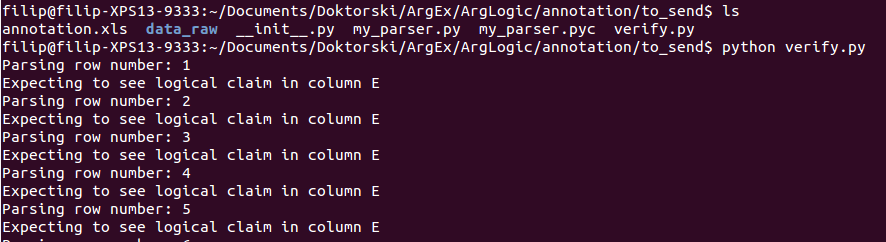
\includegraphics[scale=0.5]{struc_instructions_1.png}
	\caption{Expected output of running microstructure syntax check on entire file (\ref{item:excel}) mode}
	\label{fig:struc_instructions_all}
\end{figure}

\begin{figure}
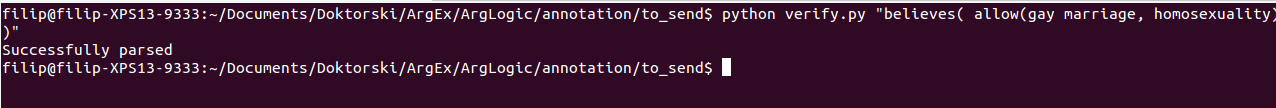
\includegraphics[scale=0.35]{struc_instructions_2.png}
	\caption{Expected output of running microstructure syntax check on a
	\label{fig:struc_instructions_2}
	single claim (\ref{item:single_claim} mode) }
\end{figure}

\noindent The script and your annotation is packaged into a zip available here. When you
unzip it, you should input your solutions in excel file \texttt{to\_send/annotation.xls}
To run it in \ref{item:excel} mode simply run \texttt{python verify.py} while
positioned in the \texttt{to\_send} directory using the command line (shown in
figure~\ref{fig:struc_instructions_all}) To run in \ref{item:single_claim}
mode, also position yourself in the \texttt{to\_send/} directory, but run as
shown in figure~\ref{fig:struc_instructions_2}.


\section{Claim segment annotation}
\label{sec:argseg_annotation}

Annotating claim segments from user comments splits the comment into claims. The
claims can be transformed into microstructures (as done to create the
microstructure dataset described in~\ref{item:microstructures_dataset}) or
formalized structures (as done to create the argument structure dataset
described in~\ref{item:structure_dataset}). Annotating segments involves
paraphrasing extracted segments to help streamline the annotation of segments
to structures. 

The task is to segment debate posts into claims. Each annotator gets a sheet in
a Google Sheets file with their name.  Column $C$ contains a user comment on
the topic of ``\textit{Should marijuana be legal}'' (MA).  The annotator needs
to carefully read the user comment, determine the stance of the comment along
with the explicit and implicit claims upon which the comment founds the
expressed stance. 

For each comment, the annotation involves:
\begin{enumerate}
\item extracting all argumentative segments of the comment as an atomic claim,
\item labeling the type of extracted segments, and
\item creating a paraphrase of the extracted segment.
\end{enumerate}
All argumentative segments should be copied to column $D$. 
Each extracted segment needs to be marked with an integer which denotes the
ordering of appearance in the post (segment $S1$, $S2$, $S3$, \dots)
All text belonging to segment $S1$ needs to be copied to column $D$, whereas
the original comment text needs to be edited to mark the segments belonging to 
the extracted segments. The beginning and end 
of the segment $Sx$ need to be marked with \texttt{<Sx>} and \texttt{</Sx>} respectively. 
Discontiguous segments are also allowed, they need to be marked with start and end tags
for each segment. Copying discontiguous segments is done by concatenating all 
instances in order of appearance. 
Column $E$ needs to contain the segment 
identifier ($S1$, $S2$, \dots). Please note that each start tag needs to be
paired with an end tag. 

\noindent Example 1: 

\begin{itemize}
  \item[] Comment: ``People are great, they have many virtues.''
  \item[] Segment $S1$: ``People are great''
  \item[] Segment $S2$: ``they have many virtues''
  \item[] Edited comment: ``\texttt{<S1>}People are great\texttt{</S1>},
  \texttt{<S2>}they have many virtues\texttt{</S2>}. ''
\end{itemize}

\noindent Example 2:
\begin{itemize}
\item[] Comment: ``People are smart and stupid.''
\item[] Segment $S1$: ``People are smart''
\item[] Segment $S2$: ``People are stupid''
\item[] Edited comment: ``\texttt{<S1><S2>}People are\texttt{</S2>} smart\texttt{</S1>}
and \texttt{<S2>}stupid\texttt{</S2>}''
\end{itemize}

\subsection*{Argumentative segment type}

The extracted segment needs to have a labelled segment type in column $F$ of
the Google sheets document. The segment needs to be classified according to two
taxonomies. First, the segment needs to be classified as either a 
\begin{enumerate}
\item fact --- statement that is true or untrue,
\item policy --- statement providing a solution or another series of questions in response to a fact,
\item value --- judgement, appraisal or evaluation. 
\end{enumerate}
Second, the segment needs to be labelled as either a 
\begin{enumerate}
\item assertion --- explicit statement or announcement or
\item rhetorical question --- question not expecting an answer. 
\end{enumerate}
More on facts, values and policies \citep{factvaluepolicy}.

\subsection*{Segment paraphrase annotation}

For each extracted segment, a paraphrase needs to be constructed. The paraphrase needs to
be assigned to column $G$ in spirit of the following principles:
\begin{itemize}
\item \textbf{Argumentativeness} -- Only argumentative text should be paraphrased; 
\item \textbf{Atomicity} -- A claim should convey a single thought; 
\item \textbf{Authority} -- Experts in claims from expert opinion should be made explicit in the paraphrase; 
\item \textbf{Brevity} -- Paraphrases should keep only the relevant argumentative content; 
\item \textbf{Canonicity} -- Canonical terms and phrases are preferred over idiomatic language;
\item \textbf{Contextuality} -- Claims should be paraphrased by considering their local and
topical context as well as their context;
\item \textbf{Declarativity} -- paraphrases should 
be in declarative form;
\item \textbf{Dereferencing} -- Pronouns and nominal  references
should be  resolved;  and
\item \textbf{Explicitness} -- Only explicitly stated
information should be paraphrased, and not whatever might be implied by the claim
\end{itemize}

\subsection*{Examples of segment annotation}

\begin{mydef}
By banning gay adoption, children in gay couple households have no legal status
should something happen to the parents, including death or serious illness.
The child cannot claim inheritances or other household assets in case of death.
If one parent dies, the second parent has no legal right to take custody or
care for the child.   A parent without legal right to a child cannot legally
register him/her for school.   Parents cannot put children on some health
insurance plans.   Parents cannot make medical decisions for the child.   * The
child has no claim to the social security or other insurance benefits of the
parent.   Gay couple parents without adoption rights do not benefit from the
generous tax deductions granted to heterosexual parents.
\end{mydef}

\noindent Extracted segments:
\begin{itemize}
\item[] \textbf{Segment1:} ``By banning gay adoption, children in gay couple
households have no legal status should something happen to the parents,
including death or serious illness.''
\item[] \textbf{Type}: Fact, assertion
\item[] \textbf{Paraphrase}: ``Children without a legal status are not
protected in case something happens to their parents''
\end{itemize}

\begin{itemize}[topsep=0.3cm]
\item[] \textbf{Segment2}: ``The child cannot claim inheritances or other household assets in case of death.''
\item[] \textbf{Type}: Fact, assertion
\item[] \textbf{Paraphrase}: ``Children without a legal status cannot claim
inheritance or other household assets in case of death.''
\end{itemize} 

\begin{itemize}[topsep=0.3cm]
\item[] \textbf{Segment3}: ``If one parent dies, the second parent has no legal
right to take custody or care for the child.''
\item[] \textbf{Type}: fact, assertion
\item[] \textbf{Paraphrase}: ``If one parent dies, the second parent has no legal
right to take custody or care for the child.'' (same)

\end{itemize}

\begin{itemize}[topsep=0.3cm]
\item[] \textbf{Segment4}: ``A parent without legal right to a child cannot
legally register him/her for school.''
\item[] \textbf{Type}: fact, assertion
\item[] \textbf{Paraphrase}: ``A parent without legal right to a child cannot
legally register him/her for school.'' (same)
\end{itemize}

\begin{itemize}[topsep=0.3cm]
\item[] \textbf{Segment5}: ``Parents cannot put children on some health insurance plans.''
\item[] \textbf{Type}: fact, assertion
\item[] \textbf{Paraphrase}: ``Parents cannot put children on some health insurance plans.'' (same)

\end{itemize}

\begin{itemize}[topsep=0.3cm]
\item[] \textbf{Segment6}: ``Parents cannot make medical decisions for the child.''
\item[] \textbf{Type}: fact, assertion
\item[] \textbf{Paraphrase}: ``Parents cannot make medical decisions for the child.''
\end{itemize}

\begin{itemize}[topsep=0.3cm]
\item[] \textbf{Segment7}: ``The child has no claim to the social security or
other insurance benefits of the parent''
\item[] \textbf{Type}: fact, assertion
\item[] \textbf{Paraphrase}: ``The child has no claim to the social security or
other insurance benefits of the parent''
\end{itemize}

\begin{itemize}[topsep=0.3cm]
\item[] \textbf{Segment8}: ``Gay couple parents without adoption rights do not
benefit from the generous tax deductions granted to heterosexual parents.''
\item[] \textbf{Type}: fact, assertion
\item[] \textbf{Paraphrase}: ``Unmarried gay parents cannot claim adoption rights
to benefit from tax deductions.''
\end{itemize}

\begin{mydef}
No it shouldnt be allowed. Marriage is when man and women get married. In the
Bible it says that its a sin for marrying your same gender and its a immoral
sin. Look at the animals they have one male and one female you dont see 2 male
horse with each other or any other animals. Look at the example animals make
learn from them.
\end{mydef}

\begin{itemize}[topsep=0.3cm]
\item[] \textbf{Segment1}: it shouldnt be allowed
\item[] \textbf{Type}: policy, assertion
\item[] \textbf{Paraphrase}: Gay marriage should not be allowed.
\end{itemize}

\begin{itemize}[topsep=0.3cm]
\item[] \textbf{Segment2}: Marriage is when man and women get married.
\item[] \textbf{Type}: fact, assertion
\item[] \textbf{Paraphrase}: Marriage is between a man and a woman.
\end{itemize}

\begin{itemize}[topsep=0.3cm]
\item[] \textbf{Segment3}: In the Bible it says that its a sin for marrying your same gender and its a immoral sin.
\item[] \textbf{Type}: fact, assertion
\item[] \textbf{Paraphrase}: According to the bible, same-sex marriage is immoral.
\end{itemize}

\begin{itemize}[topsep=0.3cm]
\item[] \textbf{Segment4}: Look at the animals they have one male and one female
\item[] \textbf{Type}: fact, assertion
\item[] \textbf{Paraphrase}: Animals of opposite sex pair up.
\end{itemize}

\begin{itemize}[topsep=0.3cm]
\item[] \textbf{Segment5}: you dont see 2 male horse with each other or any other animals
\item[] \textbf{Type}: fact, assertion
\item[] \textbf{Paraphrase}: Animals of same sex do not pair up.
\end{itemize}

\begin{itemize}[topsep=0.3cm]
\item[] \textbf{Segment6}: Look at the example animals make learn from them.
\item[] \textbf{Type}: policy, assertion
\item[] \textbf{Paraphrase}: We should learn from how animals behave.
\end{itemize}

\subsubsection*{Segment atomicity}

\begin{mydef}
I do not at all feel as God wants two men or two woman to be together, as he
has made each a man and a woman to combine and be together. However, it is our
constitutional right to make our own chices in America. What I believe should
be "exit only" is non of my business where people put things. As far as a legal
bond, we are considered "one nation under God" but , the goverment would make a
benifit from gay marriage, wether I a gree or not. Like I said we should have
the freedom to choose, we are Americans and our ancestors fought for our
freedom!!!!! Hey and I hope everyone is fighting to keep seatbelts a
choice,please keep fighting for our FREEDOM of choice!!!
\end{mydef}
This extracted segment expresses two separate ``thoughts''
\begin{itemize}
\item[] ``What I believe should be "exit only" is non of my business where people put
things.''
\end{itemize}
therefore it should be divided into two segments:
\begin{itemize}
\item[]  ``I believe should be "exit only"''
\item[] ``is non of my business where people put things''
\end{itemize}

\subsection*{Assuming too many implicit premises}

\begin{mydef}
I do not at all feel as God wants two men or two woman to be together, as he
has made each a man and a woman to combine and be together. However, it is our
constitutional right to make our own chices in America. What I believe should
be "exit only" is non of my business where people put things. As far as a legal
bond, we are considered "one nation under God" but , the goverment would make a
benifit from gay marriage, wether I a gree or not. Like I said we should have
the freedom to choose, we are Americans and our ancestors fought for our
freedom!!!!! Hey and I hope everyone is fighting to keep seatbelts a
choice,please keep fighting for our FREEDOM of choice!!!
\end{mydef}
The segment ``our ancestors fought for our freedom'' can be understood
such that the author believes that freedom refers to the freedom of choice.
This might be the case, but concluding so requires making assumptions based 
derived on implicit premises. 

\begin{itemize}
\item[] ``American ancestors fought for freedom to choose''
\end{itemize}
This paraphrase assumes ``freedom to choose''. But, the same segment can be
paraphrased not to include implicit knowledge and paraphrase in the following way 
(while also dereferencing the pronoun ``our'' to ``Americans''):
\begin{itemize}
\item[] ``Ancestors of current Americans fought for freedom of Americans.''
\end{itemize}

\subsection*{Reusing segment parts}

\begin{mydef}
As you say, "Marriage is something in particular." Its a legal union requiring
a license from a government office, not from a religious organization. That's
why gay people are fighting for "equal rights", not "equal rites."   For the
government to remain neutral on this issue, they need to stop denying gay
people the same rights as others to marry. As it is, the federal government is
anything but neutral. They deny over one thousand federal benefits to people
legally married in several states who happen to be of the same sex.
\end{mydef}
One candidate segment to extract would be:
\begin{itemize}
\item[] ``For the government to remain neutral on this issue, they need to stop
denying gay people the same rights as others to marry''
\end{itemize}
This segment actually contains three connected atomic segments (in paraphrased form):
\begin{itemize}
\item[] ``The government needs to remain neutral on this issue''
\item[] ``The government needs to stop denying gay people rights to marry''
\item[] ``Everyone but gay people have the rights to marry''
\end{itemize}


\begin{mydef}
This is the dictionary definition of marriage:   a.   the social institution
under which a man and woman establish their decision to live as husband and
wife by legal commitments, religious ceremonies, etc. Antonyms: separation.
b.   a similar institution involving partners of the same gender: gay marriage.
Antonyms: separation.   2.   the state, condition, or relationship of being
married; wedlock: a happy marriage. Synonyms: matrimony. Antonyms: single life,
bachelorhood, spinsterhood, singleness; separation.   3.   the legal or
religious ceremony that formalizes the decision of two people to live as a
married couple, including the accompanying social festivities: to officiate at
a marriage. Synonyms: nuptials, marriage ceremony, wedding. Antonyms: divorce,
annulment.   4.   a relationship in which two people have pledged themselves to
each other in the manner of a husband and wife, without legal sanction: trial
marriage.   5.   any close or intimate association or union: the marriage of
words and music in a hit song. Synonyms: blend, merger, unity, oneness;
alliance, confederation. Antonyms: separation, division, disunion, schism.
There is no mention of the reason for marriage being to Pro-create, the only
reason people should get married should be because they love each other and if
two Gay people love each other they should be allowed to marry. You can
Pro-create without getting married and I know many straight married people who
dont have Children they married because they loved each other not to have
children and Gay people should be allowed this right as well
\end{mydef}
Segment ``many straight married people who dont have Children they married
because they loved each other not to have children''
can be divided into three atomic segments:
\begin{itemize}
\item[] ``many straight married people who don't have Children''
\item[] ``many people married because they loved each other''
\item[] ``many people married not to have children''
\end{itemize}

\subsection*{Recognizing value segments}

Value segments often involve explicitly judging the value of an object.
Sometimes, the judgement can be made implicitly, but seeing explicit 
expressions should be preffered. For example: 
``People argue Gay marriage will lead to and allow
nontraditional families.'' is a factual statement, because 
the author expresses his views of public opinion. If the author expressed
his personal view like ``gay marriages lead to nontraditional families''
this could be considered a value statement, with the key part being
the word ``nontraditional'' which expresses negativity towards ``gay marriages''.
Whether there is a another view holder can influence the segment type. 
The segment ``The bible says Gay rights are immoral'' is considered a factual statement, 
whereas the segment ``Gay rights are immoral'' is considered to be a 
value segment since the segment is attributed to the author. 


\section{Prominent Claim Identification Annotation}
\label{sec:argrec_annotation}

Prominent claim identification is the task of recognizing which (from a set of
predefined) prominent claims is mentioned in a target comment and how. The goal
of the task is to label prominent claim-comment pairs with a label:
\begin{itemize}
	\item \textbf{A} -- explicitly attacks the prominent claim
	\item \textbf{a} -- vaguely/implicitly attacks the prominent claim
	\item \textbf{N} -- makes no use of the prominent claim
	\item \textbf{s} -- vaguely/implicitly supports the prominent claim
	\item \textbf{S} -- explicitly supports the prominent claim
\end{itemize}
Labeling the dataset according the guidelines below
produced the \ComArg dataset (described in section~\ref{sec:comarg}.

\subsection*{Annotation Guidelines}

There is an online discussion about ``gay rights''. The topic is ``SHOULD GAY
PEOPLE BE ALLOWED TO MARRY?''. Users post comments on the discussion forum,
which express opinions that are either for or against gay marriages. For
example: COMMENT: ``Gay people shouldn’t marry because they can’t have
children.''
In these discussions, users often refer to certain well-established arguments .
For example, typical arguments are:
\begin{itemize}
\item ARGUMENT 1: ``All people should be treated equally.''
\item ARGUMENT 2: ``Marriage should be between two believers who can produce godly offspring.''
\item ARGUMENT 3: ``Marriage is about more than procreation, therefore gay couples should not be denied the right to marry due to their biology.''
\end{itemize}

\noindent Your task is to detect WHICH arguments are used in a comment and HOW. You will
be presented with three arguments for each comment. For each argument, there
will be five check boxes, numbered 1 (DENIED) through 5 (APPROVED). 

\noindent For each argument, you need to do the following:
\begin{itemize}
\item if the comment directly denies the argument, check 1 (DENIED).
\item if the comment does not refer to the argument, check 3 (NOT MENTIONED)
\item if the comment approves the argument to make its point, check 5 (APPROVED).
\end{itemize}

\noindent You might feel that the comment approves or denies the argument, but you're not
completely certain. If you think that the argument is indirectly or partially
denied, check option 2, which is the option between DENIED and NOT MENTIONED.
Conversely, if you think that the argument is indirectly or partially approved,
check option 4, which is the option between NOT MENTIONED and APPROVED.
Note that it will often be the case that an argument is not mentioned.

Also note that if a comment and an argument express a different opinion, it
does not automatically mean that the argument is denied. For example, a comment
``Marriage is a religious institution, and the major world religions frown upon
homosexuality'' does not deny the argument ``Gay couples should be able to take
advantage of the fiscal and legal benefits of marriage''. Here, the comment and
the argument do express different opinions over the issue, but the argument
itself is not mentioned in the comment.

Consider again the example above. To detect whether and how ARGUMENTS 1-3 are
used in COMMENT, think in the following way.
In case of ARGUMENT 1: ``All people should be treated equally.''

\begin{enumerate}
\item    ARGUMENT 1 refers to human equality
\item    COMMENT does NOT refer to human equality
\item    Therefore, check option 3 (NOT MENTIONED) for ARGUMENT 1.
\end{enumerate}

\noindent In case of ARGUMENT 2: ``Marriage should be between two believers who can
produce godly offspring.''

\begin{enumerate}
\item ARGUMENT 2 implies that having children is a necessary condition for
marriage
\item COMMENT states that gay people shouldn’t marry because they cannot have
children, implying that having children is a necessary condition for marriage
\item BOTH claims are about having children and make the same point
\item therefore, COMMENT supports ARGUMENT 2
\item check option 5 (APPROVED)
\end{enumerate}

\noindent In case of ARGUMENT 3: ``Marriage is about more than procreation, therefore gay
couples should not be denied the right to marry due to their biology.''

\begin{enumerate}
\item ARGUMENT 3 implies that having children is not a necessary condition for marriage
\item COMMENT states that gay people shouldn’t marry because they cannot have children, implying that having children is a necessary condition for marriage
\item BOTH claims are about ``having children'', but COMMENT states the opposite of ARGUMENT 3
\item therefore, COMMENT denies ARGUMENT 3
\item check option 1 (DENIED)
\end{enumerate}


\section{Implicit claim annotation}
\label{app:sec:argpremises_annotation}

\subsection*{Annotation guidelines}

%This produced the argpremises dataset similarities in the (\ref{item:argpremises}).

IMPORTANT: This is essentially a reading comprehension task. While we
appreciate your opinion on this topic, this task is about analyzing OTHER
PEOPLE'S OPINIONS, not expressing your own. This is not an online survey.

\noindent There is an online discussion on marijuana legalization. The topic is: ``SHOULD
MARIJUANA BE LEGALIZED?''. You have to be familiar with of the issue: You can
get basic information about the topic 
in the footnotes\footnote{\url{http://medicalmarijuana.procon.org/}}\footnote{
\burl{http://idebate.org/debatabase/debates/health/addiction/
house-believes-cannabis-should-be-legalised}
}
Your goal is to identify whether the two sentences offered are talking about
the same thing. Please rate the SIMILARITY LEVEL for each pair of sentences:
\begin{itemize}
\item 6: very similar
\item 5 or 4: somewhat similar
\item 3 or 2: somewhat dissimilar
\item 1: not similar
\end{itemize}

\noindent Example one:
\begin{table}[h!]
\begin{tabular}{|@{\ }r@{\ \  }p{0.72\columnwidth}|}
\hline
\textbf{Sentence 1:} & \emph{Marijuana does not cause any damage to our bodies}\\
\textbf{Sentence 2:} & \emph{Consuming pot never hurt anyone}\\
\textbf{Similarity level} & 6 \\
\hline
\end{tabular}
\end{table}
\pagebreak
%\caption{User claim, the matching main claim, and the implicit premises filling the gap.}

\noindent Example two:
\begin{table}[h!]
\begin{tabular}{|@{\ }r@{\ \  }p{0.72\columnwidth}|}
\hline
\textbf{Sentence 1:} & \emph{If legalized, people will use marijuana and other drugs more}\\
\textbf{Sentence 2:} & \emph{Marijuana can be used as medicine because it showed positive effects}\\
\textbf{Similarity level} & 1 \\
\hline
\end{tabular}
\end{table}

\noindent Example three:
\begin{table}[h!]
\begin{tabular}{|@{\ }r@{\ \  }p{0.72\columnwidth}|}
\hline
\textbf{Sentence 1:} & \emph{A large portion of modern music an art has been inspired by marijuana}\\
\textbf{Sentence 2:} & \emph{Used as a medicine for its positive effects}\\
\textbf{Similarity level} & 4 \\
\hline
\end{tabular}
\end{table}


\section{Claim formalization annotation}
\label{sec:formalization_annotation}

This produced the \ref{item:structure_dataset}

\subsection{Cheat sheet}

\textbf{Task}: Transform natural language claims into logical form. Logical form needs to have:
\begin{itemize}
\item Domain individuals 
\item Claim relation
\item Modality
\item (Opinion holder)
\end{itemize}

\noindent \textbf{Domain individual} \\
Find appropriate individuals mentioned in the claim (i.e. \textit{marijuana consumers},
\textit{brain damage}, \textit{legalized tobacco}, \textit{heroin}, \textit{mafia selling marijuana}) \\

\noindent \textbf{Claim relations} \\

\begin{tabular}{| l |  p{9cm} | p{3cm}| }
\toprule
\textbf{Promotes} & 
\makecell[cc]{
\texttt{has\_antecedent + domain\_individual} \\
\texttt{promotes + domain\_individual}
}
& 
fosters, brings about, leads, forces, advances \\
\midrule
\textbf{Implies} &
\makecell[cc]{
\texttt{has\_antecedent + domain\_individual} \\
\texttt{implies + domain\_individual}
}
&
if .. then .. is \\
\midrule
\textbf{Causes} & 
\makecell[cc]{
\texttt{has\_antecedent + domain\_individual} \\
\texttt{causes + domain\_individual}
}
& causes \\
\midrule
\textbf{Suppresses} & 
\makecell[cc]{
\texttt{has\_antecedent + domain\_individual} \\
\texttt{suppresses + domain\_individual}
} &
inhibits, stops, decreases \\
\midrule
\textbf{Contradicts} & 
\makecell[cc]{
\texttt{has\_antecedent + domain\_individual} \\
\texttt{contradicts + domain\_individual}
} &
if .. then not .., is .. not a \\
\midrule
\textbf{Does not cause} &
\makecell[cc]{
\texttt{has\_antecedent + domain\_individual} \\
\texttt{does\_not\_cause + domain\_individual}
} &
causes not, does not cause \\
\midrule
\textbf{Declaration} &
\makecell[cc]{
\texttt{has\_declaration + domain\_individual}
} &
defines, exists \\
\midrule
\textbf{Comparison} &
\makecell[cc]{
\texttt{comparison\_greater + domain\_individual} \\
\texttt{comparison\_less + domain\_individual} \\
	(\texttt{comparison\_property + domain\_individual})
} &
less than, more than, greater than \\
\bottomrule
\end{tabular}
\\

\textbf{Modality} $\Rightarrow$ \texttt{has\_modality + fact/good\_value/bad\_value/policy} \\

\textbf{Opinion holder} $\Rightarrow$ \texttt{has\_opinion\_holder + domain\_individual} \\

\subsection{Examples cheat sheet}

\noindent \textbf{Promotes} \\
\begin{tabular}{p{8cm} p{8cm}}
Marijuana legalization increases crime rates. & \texttt{legalized\_marijuana promotes crime} \\
Smoking marijuana makes people happy. & \texttt{marijuana\_consumer promotes happiness}
\end{tabular}

\noindent \textbf{Implies} \\
\begin{tabular}{p{8cm} p{8cm}}
Marijuana is a drug. & \texttt{marijuana implies any\_drug} \\
	If we legalize marijuana, the government will earn money.  &\texttt{legalized\_marijuana implies government\_making\_money}
\end{tabular}
 
\noindent \textbf{Causes} \\
\begin{tabular}{p{8cm} p{8cm}}
	Marijuana consumption causes death. & \texttt{marijuana\_consumer causes death}  \\
	Marijuana legalization made government each money. & \texttt{legalized\_marijuana causes government\_earning\_money}\\
	Marijuana use alters the mind. & \texttt{marijuana\_consumer causes mind\_influential. }
\end{tabular}

\noindent \textbf{Suppresses}  \\
\begin{tabular}{p{8cm} p{8cm}}
	Legalizing marijuana hurts the balance of the economy. & \texttt{legalized\_marijuana suppresses government\_making\_money} \\
	Consuming marijuana decreases aggressive behavior. & \texttt{marijuana\_consumer suppresses aggressive\_behavior} \\
	Legalizing marijuana lowers the number of consumers. & \texttt{legalized\_marijuana supppresses marijuana\_consumer}
\end{tabular}

\noindent \textbf{Contradicts} be careful with double negation! \\
\begin{tabular}{p{8cm} p{8cm}}
	If legalization of marijuana happens, there will be no crime. & \texttt{legalized\_marjuana contradicts crime} \\
	Tobacco is not a plant. & \texttt{tobacco contradicts any\_plant}
\end{tabular}

\noindent \textbf{Does not cause} be careful with double negation! \\
\begin{tabular}{p{8cm} p{8cm}}
	Consuming marijuana does not cause death. & \texttt{marijuana\_consumer does\_not\_cause death} \\
	Legalizing marijuana never helped the government economy. & \texttt{legalized\_marijuana does\_not\_cause government\_making\_money}
\end{tabular}

\noindent \textbf{Declaration} \\
\begin{tabular}{p{8cm} p{8cm}}
	Marijuana is widely used. & \texttt{declaration marijuana\_consumer}  \\
	Marijuana should not be legalized. & \texttt{declaration illegal\_marijuana} \\
	I don’t consume marijuana.  & \texttt{declaration non\_marijuana\_consumer}
\end{tabular}

\noindent \textbf{Comparison} \\
\begin{tabular}{p{8cm} p{8cm}}
	Alcohol is more stimulative than marijuana. & \texttt{comparison\_more alcohol + comparison\_less marijuana + comparison\_property stimulative\_behavior}\\
	Heroin is worse than marijuana. & \texttt{comparison\_more herion + comparison\_less marijuana}
\end{tabular}

\subsection{Introduction}

The goal is to transform natural language claims to logical form given claims
and rules for annotation of logical form. This document explains the rules for
annotation. For example, given a claim ``The government will make a huge profit
from legalizing marijuana'' made on the topic of \textit{Drug legalization} by an author
named \textit{Fred}, we wish to transform it into logical form which would be: \\

\noindent \texttt{
author(Fred) \^{} has\_claim(Fred, c) \^{} has\_modality(c, fact) 
\^{} has\_antecedent(c, marijuana\_legalization) 
\^{} implies(c, government\_profit)
} \\

\noindent The logical form and its rules are defined by the ontology that has been
pre-created for each topic. To annotate data, you will need to use a tool named
\textit{Protege} to load the ontology. 
The outline of the annotation is: 
\begin{enumerate}
\item Open Protege and load pre-created ontology
\item Read and understand the claim individual and its entire post.  
\item Tranform the claim individual to logical form in Protege by adding properties to the claim
individual. 
\end{enumerate}

\subsubsection{Setup}

To annotate data you will need:
\begin{enumerate}
\item Download and install Protege 5, an ontology tool
\item Load provided ontology in Protege 5
\end{enumerate}
Download and install the desktop version of Protege 5. Links for Windows instructions:
\begin{itemize}
\item \url{https://protege.stanford.edu/products.php#desktop-protege}
\item \url{https://protegewiki.stanford.edu/wiki/Instal_Protege5_Win}.
\end{itemize}

\subsection{Annotation steps}

All the annotation will be done in the individuals tab of Protege. 
We discern between \textbf{domain} and \textbf{claim individuals}. 
\textbf{Domain individuals} are domain-specific as they
were mentioned previously in the debate, \textbf{claim individuals} are individuals
representing the logical form of natural language claims. 
You need to formalize natural language claims 
by recognizing claim relation and domain individuals
used to add properties to a \textbf{claim individual}. In total, you need to do \textbf{four}
steps to annotate a natural language claim:
\begin{enumerate}[label=\textbf{Step \arabic*.}, leftmargin=2cm]
\item select which domain individuals from a predefined list are used in the claim,
\item recognize which claim relation is used in the claim individual, 
\item which modality was used for the claim (\texttt{fact/value/policy}), and 
\item identify the claim opinion holder. 
\end{enumerate}


\subsubsection{Step 1: Choosing domain individuals}

We offer a list of \textbf{domain individuals} to choose from beforehand (loaded with
the ontology). We consider domain individuals well-established topics in the
debate as the authors mostly agree on them. Examples are: \textit{mafia selling
marijuana, marijuana tax, marijuana legalization, alcohol, science, obesity} \dots
They are usually nouns with adverbs. Some domain individuals are very similar
and it’s important to find the appropriate, most specific one, since you will
be offered both \textit{marijuana} and \textit{legalized marijuana}, you need to recognize which
domain individual is most appropriate given the claim. In case you don’t see an
appropriate domain individual, add a comment to the claim. We expect this to be
the case in ~15\% of the time. The goal of using domain individuals is to
transform sentences into logical with a minimal loss in meaning. Sometimes, you
will need to transform sentences from active to passive, or make verb nouns. 
For example, even though \textit{marijuana legalization}, \textit{marijuana legalizing} and
\textit{legalized marijuana} are three different concepts, we consider them the \underline{same
domain individual}. 

\subsubsection{Step 2.2: Recognizing claim relations}

Claim relations are usually, but not always, indicated by the main verb or the
conjunction in the claim. We’ve noticed four basic different claim relations
with four more subrelations (we highlight subrelations in the table with
$\rightarrow$). In the table below, we list the claim relations, possible
indicators that might hint the claim relation, the pattern in which the claim
relation might appear in natural language with respect to domain individuals
(A, B, C represent any domain individual) and an example of a natural language
claim containing the claim relation. 

\begin{tabular}{| l | p{3.5cm} | p{3cm} | p{5cm}| }
\toprule
\cellcolor{gray!25} Claim relation & \cellcolor{gray!25}Indicators &
\cellcolor{gray!25}Pattern & \cellcolor{gray!25}Example \\
\midrule
	\textbf{Promotes} & 
	Promotes, fosters, brings about, leads, forces, advances & 
	\textbf{A} promotes \textbf{B} &
\textit{Marijuana legalization improves health} \\
\midrule
	$\rightarrow$ \textbf{Implies} & 
	Implies, entails, if \dots then, is &
	\textbf{A} implies \textbf{B} &
\textit{If marijuana is legal, the crime rate will rise. } \\
\midrule
	$\rightarrow$ \textbf{Causes} &
	Causes &
	\textbf{A} causes \textbf{B} &
\textit{Marijuana legalization causes an increase in crime rate.} \\
\midrule
	\textbf{Suppresses} &
	Similar to promotes, but negative inhibitor &
	\textbf{A} suppresses \textbf{B} &
	\textit{ Marijuana hurts health. } \\
	\midrule
	$\rightarrow$ \textbf{Contradicts} &
	Does not imply, if \dots then not, is not &
	\textbf{A} implies not \textbf{B} &
\textit{If marijuana is legal, no crime will happen. } \\
\midrule
	$\rightarrow$ \textbf{Does not cause} &
	Does not cause &
	\textbf{A} does not cause \textbf{B} &
\textit{Growing marijuana at home does not stop mafia selling marijuana. } \\
\midrule
	\textbf{Declaration} &
	defines, exists &
	\textbf{A} &
\textit{Legalized marijuana exists.} \\
\midrule
	\textbf{Comparison} & 
	Is more than, has more, does less &
	\textbf{A} is more than \textbf{B} by criteria \textbf{C} &
\textit{Marijuana is less addictive than alcohol} \\
\bottomrule
\end{tabular}

In the case of promotes, its subrelation are implies and causes. Contradicts
and does not cause are subrelation of suppresses. Subrelation are \textbf{more specific}
than a claim relation meaning, if there is an implies relation, it is also a
promotes, and, if there is a contradiction or does not cause relation, it is
also a suppresses. 

\subsubsection{Step 2.2 Annotation claim relations}

Now that you’ve recognized the claim relation and domain individuals, you need
to add properties to a \textbf{claim individual}. We now explain how to annotate for
each of the four claim relations and subrelations. Promotes and suppresses are
binary (two domain individuals), declaration is unary (single domain
individuals), and comparison is ternary (three domain individuals). 

\subsubsection{Promotes}

For promotes you can choose between three options (one claim relation and two
claim subrelations):
\begin{itemize}
\item Promotes (most general) $\Rightarrow$ Promotes 
\item Implies $\Rightarrow$ Implies
\item Cause $\Rightarrow$ Causes
\end{itemize}
Implies corresponds to someone saying in the form of implication (if A then B,
A is B). Causes is when people say that one thing causes another (A causes B).
When you’re \textbf{unsure} which one to choose, but see a general pattern of (A
promotes B, A stimulates B \dots) choose promotes as a more general term.
In the case of promotes (and suppresses) you also need to specify the
\texttt{has\_antecedent} property (domain individual A in A promotes B). An example for
the claim tobacco implies cancer is below is in figure~\ref{fig:promotes_example}

\begin{figure}
	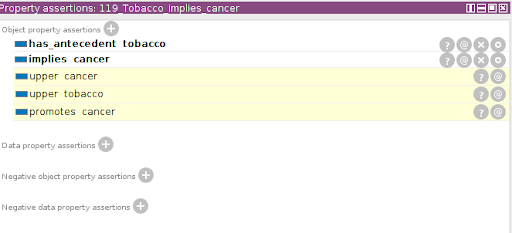
\includegraphics{promotes.png}
	\caption{Example of correct annotation for the \texttt{promotes} relation in Protege}
\label{fig:promotes_example}
\end{figure}

\subsubsection{Suppresses}

Suppresses is the \textbf{opposite} of promotes. Everything valid for promotes
also applies to suppresses, but instead of causes you have
\texttt{does\_not\_cause} and instead of \texttt{implies} you have \texttt{contradicts}.

\paragraph{Declaration}

A declaration is simply a claim stating a domain concept either exists, should
be done or is good/bad. The claim \textit{mafia sells marijuana} is annotated by adding
the \texttt{has\_declaration} with the appropriate domain individual (as seen in figure
\ref{fig:declaration_example}). 

\begin{figure}
	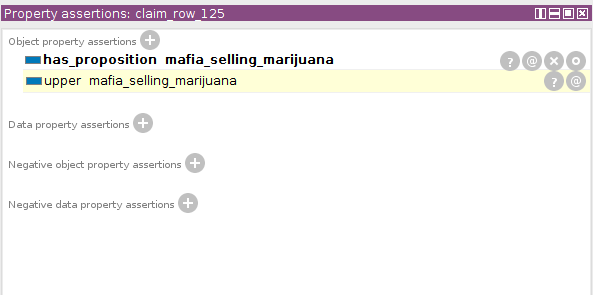
\includegraphics[scale=0.8]{has_declaration.png}
	\caption{Example of correct annotation for the \texttt{has\_declaration} relation in Protege}
\label{fig:declaration_example}
\end{figure}

\subsubsection{Comparison}

Comparisons in debates arise when someone compares two domain individuals,
usually (but not always) by saying one is better according to some feature
(which is a domain individual). The comparison pattern is A is more than B by
C. The domain individual for more is annotated with
\texttt{comparison\_greater}, less is ith \texttt{comparison\_less} and the
optional property of comparison is annotated with
\texttt{comparison\_property}. If there is no property, but an expression like
A is better than B is made, we don’t annotate \texttt{comparison\_property}.
The claim \textit{Alcohol is more influential on the mind than marijuana} is an
example annotated in the figure~\ref{fig:comparison_example}.

\begin{figure}
	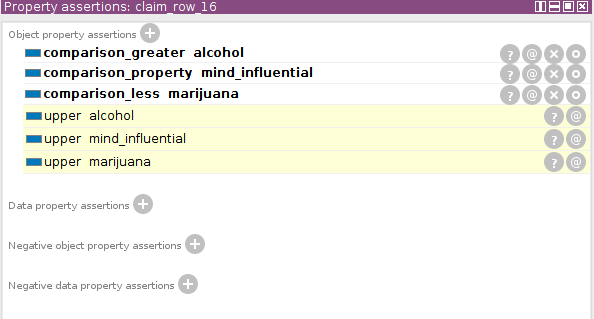
\includegraphics[scale=0.7]{comparison.png}
	\caption{Example of correct annotation for the \texttt{comparison} relation in Protege}
	\label{fig:comparison_example}
\end{figure}

\subsubsection{Step 2.3 Negation}

If you think you need to negate the selected relation, for example in the
sentence: \textit{Marijuana legalization does not promote crime} the author explicitly
states that one domain individual \textbf{does not promote} another. As not promoting \textbf{is
not always} the same as suppresses, we allow you to add negation to any
relation to reflect that. To add negation, simply select ``Negative object
property assertions'' instead of ``Object property assertions'' along with your
relation. Example on the figure \ref{fig:negation_example}. Be \underline{very careful}
when opting for negation, especially with double negation.

\begin{figure}
	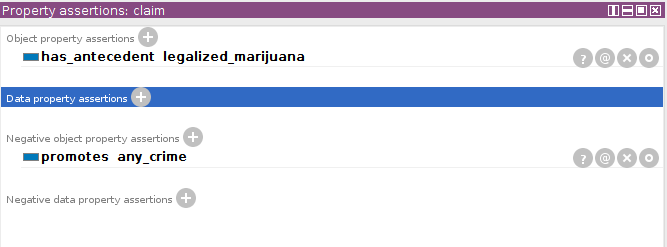
\includegraphics[scale=0.7]{negation.png}
	\caption{Example of correct annotation for negation in Protege}
	\label{fig:negation_example}
\end{figure}

\subsubsection{Step 3 Selecting modality}

We recognize that claims are made in a certain modality (way which they were
expressed with) and discern between:

\begin{itemize}
\item \textbf{Facts}:  believes/argues/thinks that claim C is true (example:
	\textit{Marijuana is legal})
\item \textbf{Policies}: A believes/argues/thinks C should be true in the
	future or should remain true  (example: \textit{Marijuana should be legal}) 
\item \textbf{Value judgement}: A believes/argues/thinks C is morally/ethically
	right or wrong
	\begin{itemize}
	\item Judging of good (example: \textit{Marijuana is great})
	\item Judging of bad (example: \textit{Marijuana sucks})
	\end{itemize}
\end{itemize}
After recognizing the modality, we need to add a property of \texttt{has\_modality} which
can be one of \texttt{fact, policy, good\_value, bad\_value}. 

\subsubsection{Opinion holder}

If the author mentions that his claim is made by someone else, we need to
annotate this information. For example, the following two claims are not made
by the same opinion holder:

\begin{enumerate}
\item Science says marijuana kills people
\item I think marijuana kills people
\end{enumerate}
For the first claim we need to add a property of \texttt{has\_opinion\_holder} to the
claim individual. The opinion holder can be any \textbf{domain individual}. In this
case, the opinion holder is science in claim 1). For claim 2), we don't need to
add a property \texttt{has\_opinion\_holder}, since the default opinion holder is the
author. 

\subsubsection{Step 5 Claim annotation comments}

This is an optional step if you can't annotate the claim for some reason. You
need to annotate the claim individual with a comment if you can't get its
logical form. \textbf{All} claim individuals \textbf{should be annotated with logical form or
commented on}. Adding a comment is done by clicking '+' in the \texttt{Annotations} and
selecting \texttt{rdfs:comment} for a specific claim. If you're missing a domain
individual (see step 1), you can simply write \textit{missing domain individual X},
where X is the domain individual you deem required to get a logical form. 
Figure~\ref{fig:comment_example} shows 
a claim individual, upper pane shows the annotations part where
you can add your comment. 

\begin{figure}
	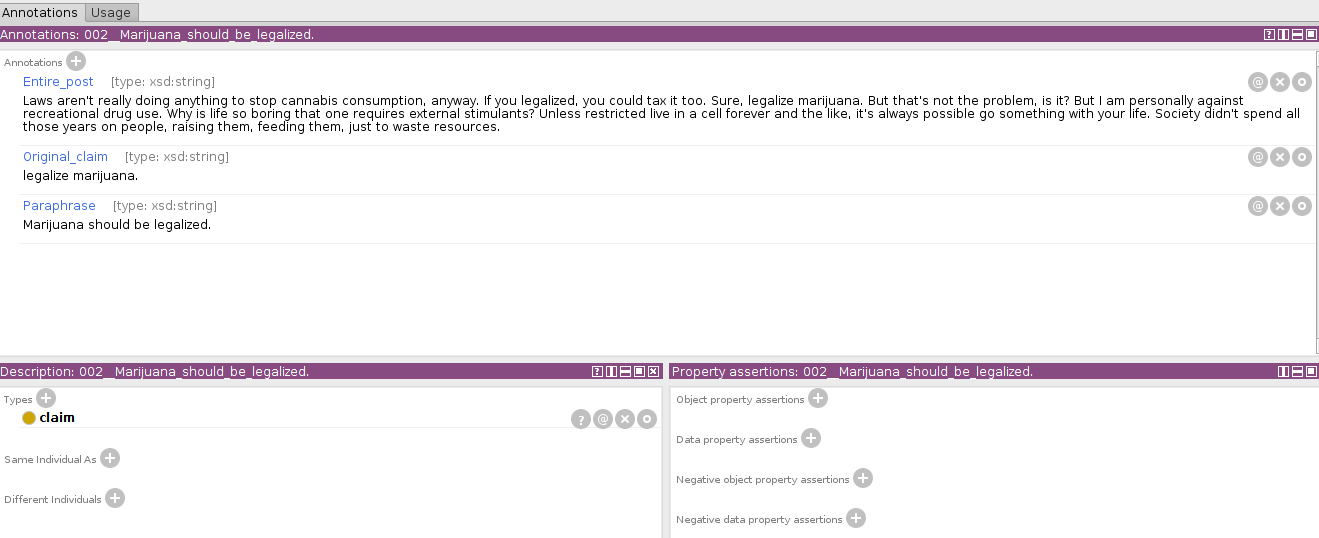
\includegraphics[scale=0.35]{comment.png}
	\caption{Example of correct annotation for adding a comment in Protege}
	\label{fig:comment_example}
\end{figure}

\subsection{Annotation Examples}

\begin{mydef}
 \textit{Marijuana legalization will increase crime rate. }
\end{mydef}

\begin{enumerate}[label=\textbf{Step \arabic*.}, leftmargin=2cm, itemsep=0.5cm]
\item You need to see which domain individuals are mentioned in the claim.
\textit{Marijuana legalization} and \textit{crime rate} are candidate noun phrases which
might be a good place to start. 
\item You see there is a will increase verb and you consult with table in step
2.1. You can narrow down the choice between promotes, implies and
causes as one thing supports another (\textit{marijuana legalization}
and \textit{crime rate}).  
\item To get the modality expressed you can work by elimination. Is there an
estimation if this is good or bad (if so, then value). Is there a
proposal of something that should be done? (if so, policy).
		Otherwise, it’s a factual information. 
\item There seems to be no mention of who is making the claim, so that should
	be the author. 
\end{enumerate}

\noindent Protege steps. 
\begin{enumerate}
\item Select the claim in Protege
\item Enter ``Object property assertions'' depending on the claim pattern identified 
\item Enter: \texttt{has\_antecedent} \texttt{legalized\_marijuana} (Step 1 \& 2)
\item Enter: \texttt{promotes any\_crime} (Step 1 \& 2)
\item Enter: \texttt{has\_modality fact} (Step 3)
\end{enumerate}

\begin{mydef}
Growing marijuana does not make mafia stop selling marijuana.
\end{mydef}

\begin{enumerate}[label=\textbf{Step \arabic*.}, leftmargin=2cm, itemsep=0.5cm]
\item Here we start from domain individuals. Marijuana and mafia related domain
	individuals seem appropriate. Looking into possible options there is a
		domain individual of \texttt{marijuana\_farmer} which seems to be the
		closest to growing marijuana. For mafia, the most similar
		individual seems \texttt{mafia not selling marijuana}
\item  Focusing on the main verb phrase ``does not make'', we can notice the
	pattern A does not cause B, hence we pick \texttt{does\_not\_cause}. We omit the
		rest of the steps as they are similar to example 1. 
\end{enumerate}
Protege steps
\begin{enumerate}
\item Select the claim in Protege
\item Enter “Object property assertions”
\item Enter \texttt{has\_antecedent marijuana\_farmer} (Step 1\&2)
\item Enter \texttt{does\_not\_cause mafia\_not\_selling\_marijuana} (Step 1\&2)
\item Enter \texttt{has\_modality fact} (Step 3)
\end{enumerate}




%\end{appendices}

%%%%%%%%%%%%%%%%%%%%%%%%%%%%%%%%%%%%%%%%%%%%%%%%%%%%%%%%%%%%%%%%%%%%%%%%%%%
\backmatter

%%%%%%%%%%%%%%%%%%%%%%% LITERATURA / BIBLIOGRAPHY %%%%%%%%%%%%%%%%%%%%%%%%%
% bibliography style file is modified IEEEtran.bst file,
% changed to suit FER's literature style
\addcontentsline{toc}{chapter}{Bibliography}
%\bibliographystyle{apalike} 
%\bibliographystyle{unsrtnat}	
\bibliographystyle{plainnat}

\bibliography{bibliography}
% \bibliography{eg_biblio}

%%%%%%%%%%%%%%%%%%%%%%% POPIS OZNAKA / NOMENCLATURE %%%%%%%%%%%%%%%%%%%%%%%
% notation and list of symbols if needed
% \printnomenclature

%%%%%%%%%%%%%%%%%%%%%%%%%%% KAZALO POJMOVA / INDEX %%%%%%%%%%%%%%%%%%%%%%%%
% optional index
%\printindex

%%%%%%%%%%%%%%%%%%%%%%%%%%%%%%%%% LOF %%%%%%%%%%%%%%%%%%%%%%%%%%%%%%%%%%%%%

\addcontentsline{toc}{chapter}{List of figures}
\listoffigures
\cleardoublepage % start new page

% insert optional list of figures
% \cleardoublepage % start new page
%%%%%%%%%%%%%%%%%%%%%%%%%%%%%%%%% LOT %%%%%%%%%%%%%%%%%%%%%%%%%%%%%%%%%%%%%
% insert optional list of tables

\addcontentsline{toc}{chapter}{List of tables}
\listoftables
\cleardoublepage % start new page

%%%%%%%%%%%%%%%%%%%%%%%%% ŽIVOTOPIS / BIOGRAPHY %%%%%%%%%%%%%%%%%%%%%%%%%%%
\renewcommand{\leftmark}{Životopis}
\chapter*{Životopis}
\addcontentsline{toc}{chapter}{Životopis}

% Životopis autora doktorskog rada treba biti napisan u trećem licu jednine, a
% opsegom ne smije prelaziti 1500 znakova (uključujući razmake).

Filip Boltužić rođen je 19. rujna 1988. u Sisku u Hrvatskoj. Prediplomski
studij računarstva završio je 2010. godine na Fakultetu elektrotehnike i računarstva
Sveučilišta u Zagrebu s temom ``Primjena algoritma kolonije pčela na kombinatoričke probleme''. 
Na istome je fakultetu završio i diplomski studij računarstva
(smjer računarska znanost) s temom ``Tehnike prikupljanja i vizualizacije
velikih skupova podataka''. 

Od listopada 2012. do travnja 2014. zaposlen je u odjelu Poslovne inteligencije 
Zagrebačke banke Unicreditgroup d.o.o. kao 
mlađi analitičar. Od srpnja 2014. do rujna 2017. zaposlen je 
u Amazon Web Services Ireland Ltd. kao razvojni inženjer. 
Od siječnja 2018. do siječnja 2020. 
zaposlen je na Zavodu za elektroniku, mikroelektroniku, računalne
i inteligentne sustave Fakulteta elektrotehnike i računarstva  
na projektu Uspostava integralnog sustava za 
upravljanje službenom dokumentacijom Republike Hrvatske kao voditelj razvoja.

Njegovi istraživački interesi obuhvaćaju područje obrade prirodnog jezika,
pretraživanja informacija i strojnog učenja. 
Član je strukovne udruge ACL (Association for Computational Linguistics). 
Govori engleski jezik.

\section*{Popis objavljenih djela}

% \subsection*{Rad u časopisima}
% 
% % TODO make enumerate
% 
% \begin{itemize}
% % \item Prezime1, InicijalImena1., Prezime2, InicijalImena2., Prezime3,
% % 	InicijalImena3., ``Naslov članka'', Naziv časopisa, Vol. X, No. Y (ili
% % 		Issue Y), mjesec i godina, str. A-B.
% \item Boltužić, F., Di Buono, M.P., Šnajder, J., Semantic-web journal
% \end{itemize}

\subsection*{Radovi na međunarodnim znanstvenim skupovima}

% TODO make enumerate
\begin{itemize}

\item Brassard, A., Kuculo, T., Boltužić, F., Šnajder, J., 
``TakeLab at SemEval-2018 Task12: Argument Reasoning Comprehension with Skip-Thought Vectors'',
12th International Workshop on Semantic Evaluation (SemEval-2018),
siječanj 2018., str. 1133-1136
\item Boltužić, F., Šnajder, J., 
``Toward Stance Classification Based on Claim Microstructures'',
Proceedings of the 8th Workshop on Computational Approaches to Subjectivity,
Sentiment and Social Media Analysis (WASSA) in conjunction with 
Conference on Empirical Methods in Natural Language Processing (EMNLP 2017),
rujan 2017., str. 74-80
\item Boltužić, F., Šnajder, J., 
``Fill the Gap! Analyzing Implicit Premises between Claims from Online Debates'',
Proceedings of the 3rd Workshop on Argument Mining in conjunction 
with 54th Annual Meeting of the Association for Computational Linguistics (ACL 2016),
lipanj 2016., str. 124-133
\item Tutek M., Sekulić I., Gombar P., Paljak I., Čulinović F., Boltužić
F., Karan M., Alagić D., and Šnajder J., ``TakeLab at
SemEval-2016 Task 6: Stance Classification in Tweets Using a
Genetic Algorithm Based Ensemble.'', Tenth International
Workshop on Semantic Evaluation (SemEval), lipanj 2016., str. 464–468
\item Boltužić, F., Šnajder, J.,
``Identifying prominent arguments in online debates using semantic textual similarity.'',
Proceedings of the 2nd Workshop on Argumentation Mining in conjunction
with 17th Annual Conference of the North American Chapter of the Association for
Computational Linguistics: Human Language Technologies
(NAACL-HLT 2019), lipanj 2015., str. 110-115
\item Boltužić, F., Šnajder, J., 
``Back up your Stance: Recognizing Arguments in Online Discussions'', 
Proceedings of the First Workshop on Argumentation Mining 
in conjunction with 52st Annual Meeting of the Association for Computational Linguistics (ACL 2014),
lipanj 2014., str. 49-58
\end{itemize}

\renewcommand{\leftmark}{Biography}
\chapter*{Biography}
\addcontentsline{toc}{chapter}{Biography}

Filip Boltužić was born on September 19, 1988 in Sisak, Croatia. 
He received his B.Sc. in Computing from the University of Zagreb, 
Faculty of Electrical Engineering and Computing in 2010 (thesis title:
``Application of the Bee Colony Optimization algorithm for combinatiorial problems'')
and M.Sc. in Computer Science from the same university in 2012 (thesis title:
``Online Analytical Processing Methods and Data Visualization'')

From October 2012 to April 2014 he was employed as a business analyst
at the Business Intelligence department of Zagrebačka banka Unicreditgroup d.o.o.
From July 2014 to September 2017 he was employed as a software 
development engineer at Amazon Web Services Ireland Ltd. From January 2018 
he is employed as a project research associate at the
Department of Electronics, Microelectronics, Computer and 
Intelligent Systems at the Faculty of Electrical Engineering and Computing on the project
% TODO UISUSD project english name
UISUSD.

His research interests include natural language processing, information 
retrieval, and machine learning. He is a member of the ACL (Association for
Computational Linguistics). He is fluent in English.


\end{document}
